%!TEX TS-program = xelatex 
%!TEX encoding = UTF-8 Unicode

% Modify the following line to match your school
% Available options include `Harvard`, `Princeton`, and `NYU`.
\documentclass[School=Harvard]{Dissertate}

% insert pdf pages
\usepackage{pdfpages}
\usepackage{caption,subcaption}

% include images
\usepackage{graphicx}
\usepackage[font=footnotesize,labelfont=bf]{caption} % reduce default caption font size
% Use Unicode characters when possible
% \usepackage[utf8x]{inputenc}
% array package and thick rules for tables
\usepackage{array}
% Remove comment for double spacing
\usepackage{setspace} 
%\linespread{2}
\usepackage{kotex} % k characters

\begin{document}

% AFTER YOU DEFEND YOU PUT YOUR CERTIFICATE HERE
% 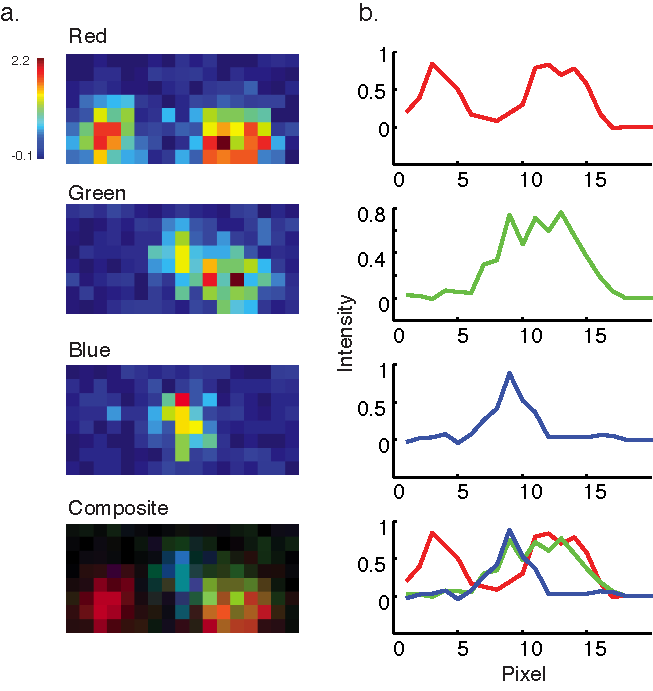
\includepdf[page=1]{figures/fullpage.pdf}
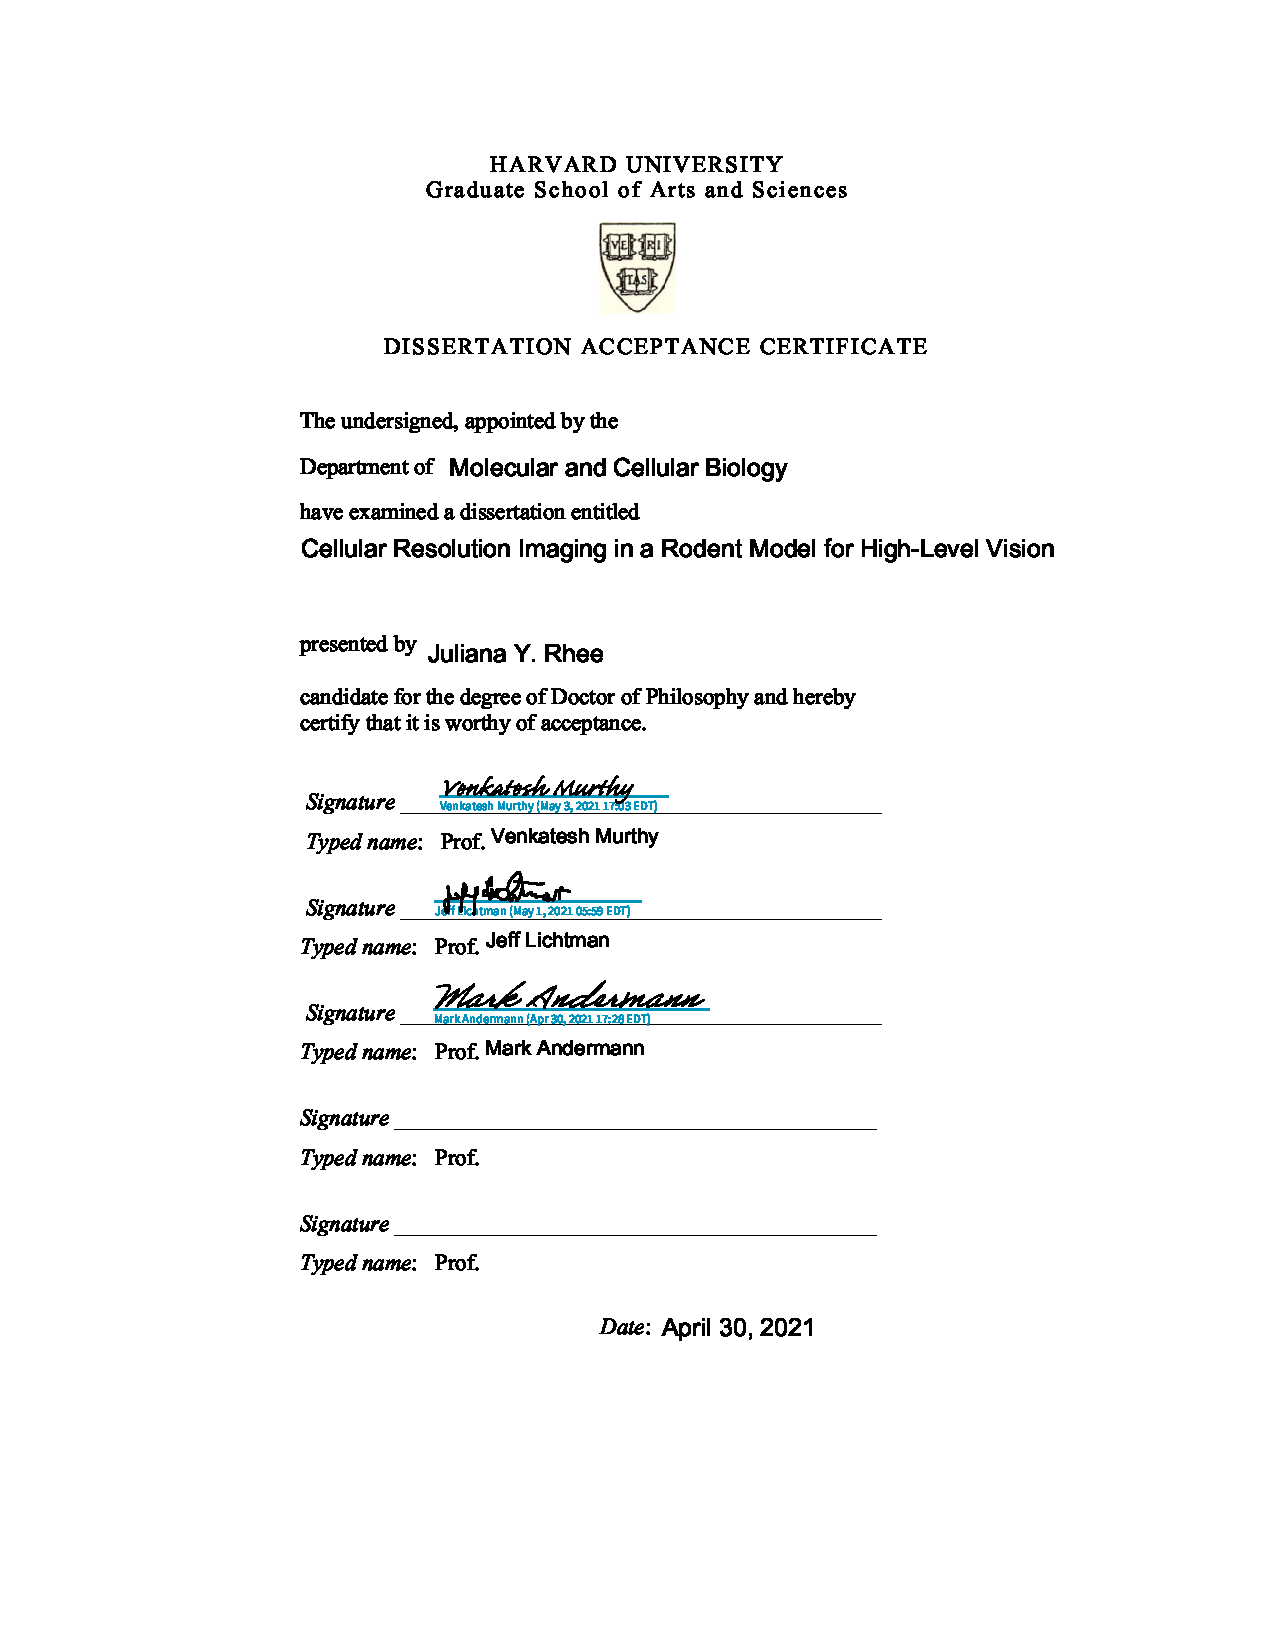
\includepdf[pages=1]{defense_certificate.pdf}

% Harvard REQUIRES you to insert an empty page here
\vspace*{0.2in}
\thispagestyle{empty} 
\clearpage

% the front matter
% Some details about the dissertation.
\title{A Rodent Model for High-Level Vision}
\author{Juliana Y. Rhee}
\advisor{David D. Cox}

% ... about the degree.
\degree{Doctor of Philosophy}
\field{Biology}
\degreeyear{2021}
\degreemonth{May}
\department{Molecular and Cellular Biology}

% ... about the candidate's previous degrees.
% \pdOneName{B.S.}
% \pdOneSchool{Boston University}
% \pdOneYear{2018}

% \pdTwoName{M.A.}
% \pdTwoSchool{Monster's Univeristy}
% \pdTwoYear{2021}
\maketitle
\copyrightpage
\doublespacing
\abstractpage
\singlespacing
\tableofcontents
%\authorlist
\listoffigures
\listofterms
\doublespacing
\dedicationpage
\acknowledgments

\doublespacing

% include each chapter...
\setcounter{chapter}{-1}  % start chapter numbering at 0
\chapter{Introduction}
\label{introduction}

% hierarchy, vision, Hubel & Wiesel, 1962, J Physiology
Our brain's visual system is an amazingly complex information processing system that transforms a stream of photons arriving at the retina into a coherent understanding of objects and surfaces in the environment~\cite{DiCarlo2007, Cox2014}. The hierarchical organization of the visual system is thought to play a key role in its ability to extract and learn about latent structure from sensory inputs. While much progress has been made in understanding the earliest stages of visual processing, our understanding of how higher visual cortical areas integrate low-level image features into representations of objects remains unclear. Understanding how the brain processes sensory information is a fundamental pillar in understanding how the brain works. 

The ability to recognize an object across the multitude of ways it can appear, \textit{e.g.}, due to viewing angle, scale, or lighting, is called invariant object recognition, or transformation-tolerant recognition. Any particular encounter with an object can cast a dramatically different image onto the retina. Despite this tremendous variation, we are able to rapidly detect, discriminate, and recognize thousands of distinct object classes with apparently little effort. The ease which we can recognize objects belies the computational complexity of this problem. We know that visual cortex successively processes input in a hierarchical cascade: lower-level areas of visual cortex tend to represent local features of the retinal image, \textit{e.g.}, oriented edges in local image patches, while subsequent higher-level extrastriate areas represent increasingly more abstract properties of the external world, \textit{e.g.}, object shape and identity. However, the computations carried out by visual cortical populations to enable this increasing complexity remains a mystery.

The mammalian visual system is the most well-studied sensory modality. Over the past 50 years\cite{Hubel1962}, the idea of a hierarchically organized system has framed our understanding of how complex behavior arises and has inspired powerful multi-layered computational networks that are capable of impressive feats\cite{Riesenhuber1999, Krizhevsky2012}. Understanding how the brain builds up visual object representations has the potential to inform not only how we perceive the things in our world, but more broadly, how a wild disarray of sensory information can be transformed into complex representations that can guide meaningful behavior.

% ----------------------------------------------------
% Primate visual system
% ----------------------------------------------------
% What do we know about visual areas (properties)
\section{The primate visual system}
In primates, visual cortex is traditionally divided into two parallel pathways: the ``ventral'' pathway runs along the ventral side of the occipital and temporal lobes, and is associated with visual shape processing, while the  ``dorsal'' pathway runs along the dorsal side of the occipital and parietal lobes, and is associated with motion processing and spatial relationships~\cite{Mishkin1982, Ungerleider1994WhatBrain, Felleman1991}. Early evidence for separate processing streams comes from studies in which lesions in different parts of these cortical paths produced contrasting effect in monkeys. For example, lesions of the inferior temporal (IT) cortex cause severe deficits in visual discrimination tasks, but have no effect on visuospatial tasks, such as visually-guided reaching or relative judgements of visual distances. In contrast, parietal cortex lesions, along the dorsal pathway, do not affect performance on visual discrimination, but severely disrupt visuospatial behaviors. As such, the dorsal path is referred to as the ``where'' pathway (concerned with \textit{where} an object is), and the ventral path is often called the ``what'' pathway (concerned with \textit{what} an object is)\cite{Ungerleider1994WhatBrain}. These pathways have also been framed in terms of a perception/action dichotomy --- that is, recognizing an object versus reaching toward it\cite{Goodale1992}.

While the two-stream framework is certainly an oversimplification, what we do know is that the primate visual cortex extracts and transforms information from one area to the next. The process begins at the retina, where photoreceptors transduce photons into neural activity, which then travels through a series of brain regions, from the lateral geniculate nucleus (LGN) and on to primary visual cortex (the first cortical area, also known as V1, or striate cortex), and beyond. Each step in this process extracts increasingly refined features, such as neurons in V1 that are selectively responsive to edges of particular orientations, and finally culminate in a group of visual areas beyond V1, collectively called ``extrastriate'' cortex --- here, neurons respond selectively to higher-order visual features, such as objects, faces, or motion\cite{Orban2008, DiCarlo2012}. 

Visual object recognition in primates is thought to emerge through these sequential processing stages across the ventral visual pathway~\cite{Rust2010SelectivityIT, DiCarlo2007, DiCarlo2012}. From early to late stages of the hierarchy, single neuron properties vary systematically. In V1, receptive fields are smaller and cells are optimally stimulated by oriented edges or gratings\cite{Hubel1968}. In subsequent stages, receptive field sizes get larger, while selectivity for complex shapes increases~\cite{Desimone1984, Logothetis1996}. At the same time, neurons in later, higher-level areas exhibit tolerance to identity-preserving transformations: in these highest stages of the ventral pathway, inferotemporal or IT cortex, cells selectively respond to a given object regardless of changes in size, location, or particular appearance on the retina~\cite{Tanaka1996, DiCarlo2012}. Some studies even report neural activity highly specific for behaviorally-relevant categories, such as faces\cite{Kanwisher1997, Tsao2006} and scenes\cite{Epstein1998}.

% ----------------------------------------------------
% Methods for population recordings
% ----------------------------------------------------
% What's holding us back!
\section{Methods for population recordings}
While much work on the visual system has been done studying the responses of single neurons, we lack a complete understanding of how populations of neurons work together to represent the external world. Our understanding of the nature of computations that take place in visual cortical populations has been partially limited by the tools at our disposal to probe neuronal populations. Decades of research in the primate visual system have relied on investigators sampling from neuronal populations in the ventral visual pathway of monkeys using single microelectrodes or electrode arrays, but these techniques have several fundamental limitations. First, they are only able to sample from a comparatively small number of neurons at time, generally requiring the assembly of serially-sampled ``pseudo-populations'' in order to explore population coding. Second, electrophysiological recording techniques typically do not allow the same populations of neurons to be studied over long periods of time. In some cases, a small number of neurons can apparently be isolated for days in a chronic preparation; however, it is usually impossible to be certain that these cells are the same across days. 
% Ephys:
% (Jun et al., 2017 (neuropixels); 
% Siegle et al., 2019 --Nature, 2021,. (hierarhcy, Nature)
% Stringer et al., 2019a -- spontaneous bebaviors, Science

% ca imaging: 
% (Sofroniew et al., 2016; -- meoscope, elife
% Stringer et al., 2019b --high-dim geometry, Nature
% Weisenburger et al., 2019). --- alipasha, Cell
A major goal of systems neuroscience is to explain how complex behaviors arise from the combined activity of many individual neurons. Thus, advances in population recordings, which allow the activity of many neurons to be captured at the same time, have dramatically expanded the scope of questions that researchers are able to ask. Extracellular electrophysiology and two-photon optical imaging are the most popular methods for recording neural populations, due to their single-cell resolution, relative ease of use, and scalability. Within the last five years, large-scale recordings of hundreds and even thousands of neurons are becoming increasingly standard using electrophysiology \cite{Steinmetz2019, Siegle2021} and optical imaging \cite{Stringer2019a, Weisenburger2019, Sofroniew2016}. With rapidly growing advancements in genetic tools, hardware design, and computational power, we are in an unprecedented time to be studying neural circuits and behavior. 

Today, one of the greatest advantages of optical imaging is cellular resolution access to large neural populations. To be able to visualize single neurons as a population in awake animals is immensely powerful, especially in concert with sophisticated manipulation techniques, such as multi-channel optogenetics and holographic light stimulation\cite{Gill2020}, and genetically-defined targeting of specific populations of cells. In species in which these tools are available, such as mice, we have been able to gain unprecedented access to genetically defined cell types and their role in circuit functions\cite{Luo2008, Luo2018, Huberman2011}. In combination, these features allow one to measure and manipulate the same neurons in awake, behaving animals across large numbers of stimuli and trials over the course of weeks and months. 


However, primates are a difficult animal system in which to use existing tools for probing neuronal populations, such as \textit{in vivo} 2-photon calcium imaging \cite{Ohki2005}: monkey cortex is 2.5mm thick on average\cite{Koo2012}, making it difficult to image much beyond layer II, due to optical scattering limits. In addition, monkeys are capable of significant head movement even when head-fixed, and even at rest their brains move significantly due to pulsatile motion, which complicates imaging. At the same time, the complexity of the monkey ventral visual pathway, albeit more similar to the human visual system, is more challenging to understand relative to simpler systems. As a result of all of these factors, a growing number of investigators have turned to simpler alternative models to explore a variety of ``high-level'' sensory and cognitive functions in less complex systems\cite{Brunton2013, Miller2017TwoStep, Aronov2014, Glickfeld2017}).

% ----------------------------------------------------
% Rodent Models for Vision
% ----------------------------------------------------
\section{Rodent Models for Studying Vision}
Over the past ten years, rodents have emerged as a powerful system for studying visual circuits. Among rodents, this is particularly true for mice, as an important driving force has been the rapid development of a large array of genetic tools for analyzing connectivity and probing and controlling activity in neural circuits\cite{Luo2008, Luo2018}. Furthermore, rodents offer excellent experimental accessibility. They have a lissencephalic cortex, which means that their cortex is smooth and does not have the characteristic folds of gyri seen in primate cortex. This is particularly advantageous for optical imaging techniques, as more of the brain is accessible right at the surface. Second, rodents cost much less than primates to keep in the laboratory and are easier to house in large numbers, which means access to larger sample sizes in a given experiment. On the other hand, mice and rats are have much lower visual acuity, which raises the possibility that their visual system is fundamentally different from the visual systems of primates. 

%Evidence that rats are good at stuff
To date, the majority of studies of higher-level visual processing have been done in non-human primates, largely because they are similar to humans, and because it had been erroneously assumed that simpler model systems lack sophisticated visual systems. However, increasing evidence suggests rodents possess rather sophisticated visual machinery that would make them a tractable model for studying multi-level visual processing. A number of studies have demonstrated that many basic properties of visual function, at least from the retina and up to V1, are present in rodent visual cortex\cite{Huberman2011}. Within V1, several circuits underlying a range of cortical computations have been found, including orientation selectivity \cite{Ko2011, Lien2013}, surround suppression\cite{Adesnik2012}, and gain control\cite{Atallah2012}. 

Beyond V1, there are a number of extrastriate areas in both mice\cite{Andermann2011, Marshel2011, Juavinett2017} and rats\cite{Espinoza1983, Coogan1993}. Anatomical evidence suggests a hierarchical organization\cite{Wang2007, Wang2011}, as the connectivity patterns of extrastriate area are suggestive of homology with the dorsal and ventral pathways in primate cortex. Over the last decade, a growing number of functional studies have ventured further into extrastriate cortex, and have begun to systematically characterize basic response properties of these visual areas in the mouse\cite{Andermann2011, Marshel2011, Glickfeld2013, Glickfeld2017, DeVries2020, Siegle2021}. Visual areas corresponding to a putative dorsal pathway in mice contain neurons that are particularly tuned for motion\cite{Andermann2011, Marshel2011, Glickfeld2013} and exhibit sensitivities to motion processing in specific portions of the visual field\cite{Sit2020}. In the putative ventral stream, several studies have found less motion sensitivity and greater tuning for higher spatial frequencies\cite{Glickfeld2013, Tohmi2014}, properties that would facilitate visual shape processing. 
% 
Despite the many similarities between rodent and primate visual systems, there are also striking differences. For example, primates have a fovea, a specialized region that takes up a tiny portion of the retina but contains the highest density of photoreceptors\cite{Perry1985}, while rodents do not. Primates use foveal vision for high contrast, high acuity tasks, such as a reading or detecting small objects. Within V1, both species exhibit the hallmark property orientation tuning, but differ in spatial organization: in primates, cells preferring a particular orientation are organized in a ``columnar'' structure, while in rodents, orientation selectivity forms a salt-and-pepper organization\cite{Ohki2005}. In addition, in both rats and mice, projections from V1 extend to areas that process motor and other non-visual information, while in the primate visual system, extrastriate or higher-order areas project to regions that process non-sensory information. 

% ----------------------------------------------------
% Rodent Models for Vision
% ----------------------------------------------------
\section{High-Level Vision in Rodents}
In traditional visual neuroscience, mice were ignored for a long time under the assumption that they do not exhibit interesting visual behaviors --- however, the immense power of their experimental and genetic tractability has renewed interest in exploring the extent and range of their visual capacities, such as visually-guided hunting behavior\cite{Hoy2016, Meyer2020, Michaiel2020}. In contrast, rats stand out among rodents because there is a long and rich history of studies of their visual behavior. In the 1930s, Lashley and others published a series of studies demonstrating the ability of rats to perceive and discriminate visual shapes\cite{Lashley1912, Lashley1930a, Lashley1938}. In the 1970s, a landmark study by O'Keefe and colleagues demonstrated visually-guided spatial navigation\cite{OKeefe1971}. Compared to mice, rats are also not strictly nocturnal, have higher visual acuity\cite{Prusky2000}, and perform better and learn quicker on many visual and cognitive tasks\cite{Whishaw1995}. In the context of visual object recognition behavior, several groups have since built upon these studies, and have shown that rats rely on a range of visual strategies to perform object recognition tasks\cite{Zoccolan2009, Tafazoli2012, Vermaercke2012, Alemi-Neissi2013, Vinken2014}.

% Specific to object recognition 
Importantly, recent studies have also identified a collection of visual areas along the lateral, posterior edge of rat cortex that may exhibit several features that have been considered hallmark characteristics of the primate ventral pathway. Specifically, starting from primary visual cortex (V1), these areas area the lateromedial area (LM), the laterointermediate area (LI), laterolateral area (LL), and the occipitotemporal
cortex (TO). In support of anatomical evidence suggesting a hierarchical progression of low to high across these areas\cite{Coogan1993, Wang2012NetworkCortex, DSouza2020}, a growing body of functional evidence has identified several hallmark features of neurons in these visual areas of the rat that are reminiscent of important properties of the primate ventral pathway. For example, studies have found an increase in stimulus-evoked response latency across these areas\cite{Vermaercke2014, DSouza2020}, suggesting a sequential processing of stimulus information.

In the context of visual object recognition, there are several hallmark features of the primate ventral pathway that have been found, to varying degrees, in rat lateral cortex. The most consistent of these is an increase in receptive field size, from V1 to LM, and on\cite{Vermaercke2014, Tafazoli2017}. Less clear, is the extent to which shape selectivity and transformation tolerance across rat lateral cortex clearly maps onto areas of the primate ventral path. For example, several groups have found that more lateral areas are better at decoding object identity than V1, even across identity-preserving transformations\cite{Tafazoli2017, Vermaercke2014, Froudarakis2020}. However, in contrast to the primate ventral path, Vermaercke and colleagues found that this increasing discriminability was only found when moving objects were used\cite{Vermaercke2014}. Moreover, in contrast to the primate visual system, the same group also found an increasing selectivity for drifting gratings. In another study, Vinken and colleagues found that although areas LI and LL did a better job at discriminating natural images than scrambled images, they did not find category-selective representations, as might be expected in a  higher-level area of visual cortex\cite{Vinken2016}. 


% Not enough tools in rats, even tho their behavior is awesome
\section{Goals of the present study}
The many similarities between monkey and rodent visual systems, from low-level areas like V1 to primate IT and putative higher-level rodent counterparts, such as LI or LL, suggest that rodent extrastriate areas can serve as a valuable complement to monkey visual models --- however, many aspects of the rodent visual pathway remain to be characterized in detail. Although a large body of scientific research, including visual object recognition, relies on the rich behavioral repertoire of rats, it has proved to be more challenging to fully leverage recent developments in optical imaging and genetic tools in the rat, as it has been done with great success in smaller animals like mice\cite{Luo2018}. Notably, all prior studies of neural processes underlying object recognition in rats have relied on single-unit responses and acute electrophysiology in passively viewing or anesthetized animals. Few or no paradigms exist for large-scale cellular resolution imaging of extrastriate cortex in awake, head-fixed rats (though see V1 recordings in \cite{Greenberg2008}). 

One of the biggest challenges in applying cellular resolution optical imaging approaches to rodents has been head-restrained preparations, which have become relatively standard in studies of mouse visual cortex. While head-fixed preparations are routinely used in mice, this is not the case in rats. Rats are much bigger than mice, and their larger size makes them harder to restrain. Moreover, they can cause sufficient force to severely damage themselves or produce prohibitively large artifacts for cellular resolution imaging. As such, most studies using head-fixed rats rely on electrophysiology, or freely moving approaches with limited optical access\cite{Scott2013}. Furthermore, the lateral position of candidate object recognition areas makes optical access all the more challenging, and rat imaging studies have been restricted to medial V1\cite{Greenberg2008, Ohki2005}. Nonetheless, head-fixed preparations afford certain experimental advantages, such as restrained movement, precise stimulus control, and longitudinal studies that can track the same neurons over long timescales. 

% Given likely differences in response characterizations between optical imaging and and electrophysiology approaches\cite{SiegleReconcilingElectrophysiology}, it is challenging to interpret results and attribute possible differences to methods as opposed to species-specific adaptations. 

% Even among rodents, there may be species-specific differences in how analogous brain areas are to parts of the primate ventral stream. For example, in mice, areas LM and AL seem to contain the most object-specific, view-tolerant information\cite{Froudarakis2020}, while studies in rats point to areas LI, LL, or even TO\cite{Vermaerke2014, Tafazoli2017}. Such differences may be due to behavioral differences in visual capacities between rats and mice, \textit{e.g.}, visual acuity\cite{Prusky2000}, how diurnal or nocturnal they are, and the extent to which they rely on visually-guided behavior\cite{Whishaw1995, Whishaw1996}. Moreover, even among rat studies, paradigms differ in stimulus set, recording techniques, and behavior states. 

% PRESENT STUDY -- what am i doing and why.
The recent emergence of the mouse as a powerful system for studying visual circuits has largely been driven by the ability to apply a wide array of powerful genetic tools for circuit dissection, along with technological advancements that allow simultaneous acquisition and manipulation of large neuronal populations in awake animals. On the other hand, despite the long history of rich behavior studies in the rat, and its continued popularity and value as a model system in many other fields of biomedical research, many of those existing tools have not yet been leveraged in rats. An overarching goal of the present study is to combine these two threads. Here, we aim to bridge the gap between neural circuit access and rich behavioral capacities in the rat. We demonstrate reliable, high-throughput cellular resolution optical imaging in awake, head-fixed rats for the first time, and show the feasibility of applying the powerful tools available in systems neuroscience to a rodent model of high-level vision. 

In Chapter 1, we develop a system for automated, high-throughput training of visual behaviors in rats. This work builds off of previous work showing visual object recognition capacities of rats, and is inspired by the many high-throughput behavior systems developed for testing non-vision-specific tasks in rodents. We describe an open-source, modular, and high-throughput system in which large cohorts of animals can be trained on complex visual behaviors. In this chapter, we also describe rats' perceptual choices in response to visual stimuli for which we will characterize neural responses in later chapters. In Chapter 2, we describe our efforts to engineer systems for optical imaging in head-fixed rats. As this work is the first time rat lateral cortex has been studied with cellular resolution imaging, in Chapter 3, we present a systematic survey of basic response properties in areas V1, LM, and LI. We describe the macro- and micro-scale organization of these areas in the context of a range of stimulus classes. While Chapter 3 focuses on responses to simple features, in Chapter 4, we return to the object stimuli used to probe the visual behavior of trained rats. Here, we characterize population responses in rat visual cortex to examine how neural circuits encode feature variations that either preserve object identity or alter object identity. Finally, we conclude with a chapter that discusses the developments and findings of the previous chapters, and places them in the context of previous findings, while considering both caveats and future work that can build from the present study.

This work aims to fill gaps in our current understanding of the rodent visual pathway that will further enhance the rodent as an animal model. Taken together, this work offers the potential for a new, powerful, complementary animal model for the study of high-level vision.



%%%% 

% Vision is critical for guiding behavior in species throughout the animal kingdom. Though nonhuman primates have been the classic model for vision, alternative systems offer a way to reveal general principles of visual processing as well as species-specific adaptations. Advances in imaging techniques and genetic tools have made genetically accessible animals, like mice, valuable systems for understanding neural circuits of vision. In contrast, although rats have long been studied for visually-guided behaviors, large-scale cellular resolution access to their visual cortex has proved to be far more challenging. Here, we aim to bridge the gap between neural circuit access and rich behavioral capacities in the rat. We characterize the functional organization of a subset of visual areas for the first time with cellular resolution imaging in awake, head-fixed animals. 


% REFREF WHY head fixed


% TABLE, prev studies
% \begin{tabular}{ |p{3cm}|p{3cm}|p{3cm}|  }
% \hline
% \multicolumn{3}{|c|}{Country List} \\
% \hline
% Country Name     or Area Name& ISO ALPHA 2 Code &ISO ALPHA 3 \\
% \hline
% Afghanistan & AF &AFG \\
% Aland Islands & AX   & ALA \\
% Albania &AL & ALB \\
% Algeria    &DZ & DZA \\
% American Samoa & AS & ASM \\
% Andorra & AD & AND   \\
% Angola & AO & AGO \\
% \hline
% \end{tabular}

% \begin{savequote}[75mm]
% Does this shit even work?
% \qauthor{A Tired Grad Student}
% \end{savequote}

\chapter{High-throughput behavior in rats}
\newthought{The laboratory rat \textit{Rattus norvegicus}} was the first mammalian species domesticated for scientific research\cite{Jacob199}, and has since been the most widely studied specie in biomedical research. In the lab, rats can be trained to perform cognitively demanding tasks. They have a long history as laboratory models for the behavioral study of cognitive capacities, including decision-making\cite{Brunton2013, Raposo2012, Miller2017TwoStep, Piet2018RatsEnvironment}, working memory\cite{Bratch2016}, and spatial navigation\cite{OKeefe1971, Whishaw1995, Aronov2014}. 

One of the most widely used tools for studying animal behavior in the lab is the operant conditioning chamber. With the conditioning chamber, the experimenter gradually shapes the animal's behavior until the desired task is learned. Like most rodent behavior experiments, tests of visual object recognition rely on operant conditioning. Technological developments over the past ten years have enabled experiments to use these traditional conditioning boxes in computer-controlled systems that allow for automated and high-throughput training. 

Automated training methods are more efficient because they require little to no hands-on involvement from the experimenter. Animals can be placed into chambers by staff who are unbiased about the particular study's goals or they can simply live in the boxes with automatically or remotely controlled training regimes\cite{Qiao2018, Poddar2013, Miller2017Twostep}. Thus, high-throughput systems not only allow for more systematic and less biased experiments, but also allow many animals to be trained and studied in parallel. Higher-throughput studies provide statistical power difficult to achieve with small-scale animal cohorts and importantly, have the potential to provide a readily available source of animals for physiological access or perturbation studies. These advantages are particularly important for behavioral tasks that are complex and require long training schedules.

In 1930, Karl Lashley\cite{Lashley1930} described a wide range of visual behaviors in rats using what is now a classic two-choice paradigm\ref{fig:FIG?}. In his version of the rig, Lashley tested rats' visual shape recognition capacities by training them to select a particular gate or door depending on what stimulus it showed in order to access a hidden food reward. Fast-forward $\sim$80 years, experiments have relied on similar training rigs to test rats on visual object recognition tasks\cite{Zoccolan2009, ETC}. While most studies using monkeys rely on about 2-3 animals, standard rat vision studies use ~4-6 animals per experiment\cite{Vermaercke2012, Tafazoli2012Transformation-TolerantPriming}.

In contrast, several groups studying rats outside of traditional visual neuroscience have pushed the bounds to demonstrate the power of high-throughput rat behavior. Of note, Brody and colleagues use highly complex tasks that take rats months to learn, and have developed massively high-throughput behavior systems that train many rats in parallel on various acoustic decision-making and working memory tasks\cite{Miller2017TwoStep, Brunton2013RatsFrom}. In motor skill learning, Olveczky and colleagues have built high-throughput, fully-automated systems for home-cage training\cite{Poddar2013}. In mice, a growing number of high-throughput systems now exist\cite{Qiao2018}). Inspired by the power of large-scale behavior systems, our goal was to take existing visual behavior paradigms in rats and adapt them for high-throughput, automated training. 

% This is a math equation that can go here for now.
% $$\zeta = \frac{1039}{\pi}$$

% %%%%%%%%%%%%%%%%%%%%%%%%%%%%%%%%%%%%%%%%%%%%%%%%%%%%%%%%%
% Results
% %%%%%%%%%%%%%%%%%%%%%%%%%%%%%%%%%%%%%%%%%%%%%%%%%%%%%%%%%
% fig:openratbox
% fig:basic_training
% fig:behavior_generalization

% ---------------------------------------------------------
% OpenRatBox -- the hardware.
\section{OpenRatBox: An open-source platform for high-throughput behavior}
Our approach was to design a visual behavior system that was reproducible, low-cost, and modular. It was critical to design training boxes that would be straightforward to reproduce, not only to maintain constancy from one box to the next, but also to facilitate widespread use both within the lab and across labs. Systematization across research groups can be immensely powerful, especially for studying highly complex, multi-modal processes like decision-making, as exemplified by the International Brain Laboratory\cite{IBL} and the Allen Brain Institute\cite{REFREF}.

In order to build behavior boxes at a larger scale, we relied on low-cost, readily accessible components and open-source software for experimental control. While it is possible to build a highly sophisticated and customized apparatus that meets the particular demands of a given experiment, it can be extremely costly and hard to adapt for other experiments or impossible to use by other labs. In contrast, designing a low-cost system that relies on open-source technology allows it to be more accessible as a tool that can benefit others, while also allowing for continued improvements and new adaptations. Modularity is important because a given behavior can be tested under different regimes. For example, two commonly used behavior choice paradigms are Go/No-Go and two-alternative forced choice (2AFC) tasks. These paradigms offer different advantages and disadvantages, and also have different hardware requirements: while Go/No-Go paradigms only require a single reward port or choice manipulandum, 2AFC and other multi-choice tasks require at least two. 

% FIGURE 1.1 OpenRatBox Schematic
\begin{figure}[t!]
    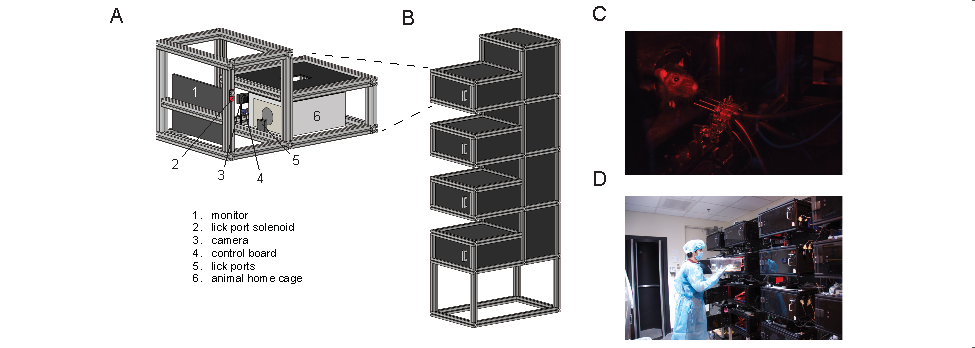
\includegraphics[width=\textwidth]{figures/chapter_1/fig_1-1_openratbox/fig_1-1_openratbox_compressed.pdf}
    \vspace{.1in}
    \caption[OpenRatBox]{OpenRatBox: Open-source, automated, high-throughput training. \textbf{A.} Schematic of one training box. Numbers denote relevant parts. 
    \textbf{B.} Left, A full tower assembly of four identical training boxes. \textbf{C.} A photograph of a rat in a training box equipped for a three-port task. \textbf{D.} A photograph of a room of towers used to train the animals in the present work. An experimenter is shown loading an animal in its home cage into the training box.  
    \label{fig:openratbox}}
\end{figure}

The overall design of each box is identical, and experiment-specific adjustments are made with modular components. The main vestibule of each unit houses the animal's cage and all hardware needed to collect the animal's response and monitor its behaviors (Figure\ref{fig:openratbox}A). Each unit is equipped with a small computer that allows as many experiments to be run independently and in parallel as there are boxes. The external frame is composed of aluminum extrusion bars and custom-cut acrylic paneling that fits into the railing slots of the bars, such that an arbitrary number of boxes can be built on top of the next, limited by the available vertical space. In our behavior rooms, we had enough space for towers composed of 4 stacked units (Figure\ref{fig:openratbox}B). All the training boxes are controlled and monitored by a control computer that runs a client (MWorks) that interfaces with the servers running in each behavior box. 

Within a given unit, there are two partitions. The monitor is mounted on a partition separate from the main vestibule in order to keep it clean and protected (for example, from chewing, or stray water droplets and bedding). The animal has visual access to the monitor through a window separating the monitor from the main vestibule that holds the cage. The cage itself is held in place with two spring-loaded latches that allow the cage to be loaded into the same relative position, if necessary. The cage locking mechanism was adapted from a commercially available, self-standing animal cage rack, in which each cage is locked into the air circulation and filtration system. The box is thus designed to support fully live-in animal behavior training. 

During visual behavior sessions, the animal has access to the reward ports and monitor through a small window placed at one end of the home cage. In the case of live-in training, the window can be gated shut during non-training times, if desired. Mini extrusion bars are screwed directly into the acrylic floor of the main vestibule around the animal's access window. This effectively creates a mountable rail system for attaching experiment-specific components, such as reward ports, USB cameras, and IR detectors (Figure\ref{fig:openratbox}A). As such, any modifications specific to a paradigm (\textit{e.g.}, one reward port or three reward ports) could be easily attached or removed from one box to the next. All wiring feeds through small access holes cut into the acrylic pieces embedded into the extrusion bars, as does tubing for water delivery of rewards. Attached to each box is a small computer (Mac Mini, though others are possible) that runs the experiment (visual stimulation, I/O control, and so on). 

In addition to specific behavior task constraints, such as 1 reward port or multiple, a desirable feature of behavior systems is the ability to combine them with physiology or neural manipulations. The behavior rigs are modular enough that rats with tethered cables can also be housed in the boxes, as there is sufficient room for an access port and a commutator that can hold the cabling attached to the animal's head. Thus, the entire system can be equipped for neural stimulation and recording in tethered rats. The spacing between the stacked boxes can be kept as is or adjusted for a commutator system that carries a cable from the animal's head through a hole in the acrylic ceiling of the main vestibule (Figure\ref{fig:openratbox}D). Though we tested both Go/No-Go and two-choice behavior paradigms, we selected the latter for the remainder of our behavior studies (see Discussion) as this is a well-established paradigm used to test visual object recognition behavior in rats\cite{Lashley1930, Zoccolan2009, Prusky2000}.

% ---------------------------------------------------------
% OpenRatBox -- the functionality (high-throughput training)
\section{High-throughput behavior training}
We trained rats to perform a simple, two-category object discrimination task\cite{Zoccolan2009} (Figure\ref{fig:basic_training}\textbf{A}). This is a three-port paradigm in which rats lick the center port to initiate trials, and one of the two flanking ports to indicate which object is on the screen. Rats initiated each trial by licking the middle of three capacitive lick ports, which triggered the appearance of one static visual object (1 of the two object categories) on the screen (see Methods for details). The rats indicated which visual object was present by licking one port, \textit{e.g.}, the left port, for object A, and the other \textit{e.g.}, for object B, with stimulus-port mappings counterbalanced across animals (Figure\ref{fig:basic_training}\textbf{B}).

% FIGURE 1.1 Basic training
\begin{figure}[t!]
    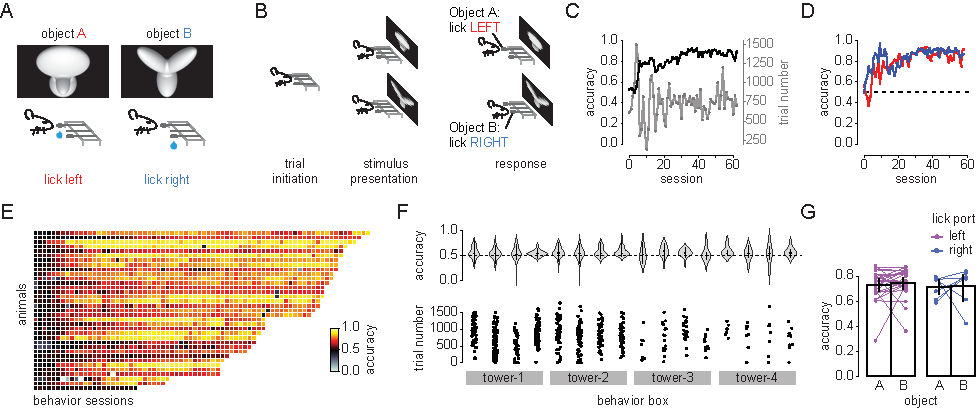
\includegraphics[width=\textwidth]{figures/chapter_1/fig_1-2_basic_training/fig_1-2_basic_training.pdf}
    \vspace{.1in}
    \caption[High-throughput training]{High-throughput training on a simple two-alternative choice task. 
    \textbf{A.} Logic of the basic, two-category object discrimination task. 
    \textbf{B.} Trial structure (adapted from \cite{Zoccolan2009}). Animals trigger a trial by licking the center port. After a variable delay, a stimulus appears on the screen, and the animal licks one of the ports to indicate it sees object A, or the other lick port to indicate it sees object B. 
    \textbf{C.} Example training data from one rat. Black, overall accuracy as a function of training session number. Gray, Number of trials completed in each session. 
    \textbf{D.} Accuracy for each of the two objects for the example rat shown in \textbf{C}. Colors correspond to each of the two object identities.
    \textbf{E.} Overall accuracy for a large cohort of animals (N=33 rats) as a function of training session. 
    \textbf{F.} \textit{Top}: Accuracy for each box and each tower. Each group of 4 points, indicated by the labels underneath, represents one tower composed of 4 boxes (4 towers shown, tower-1, tower-2, etc.). The relative position of each group within the tower represents the same physical location in each tower (top, second from the top, etc.). \textit{Bottom}: Number of trials performed per session for each box and tower. Each dot denotes a session for an animal. Organization of grouped points is the same as the upper panel (corresponding to boxes and towers). 
    \textbf{G.} Performance split by stimulus-port mapping and object identity. Red, accuracy for object A. Blue, accuracy for object B. Portmap 1 and 2 denote whether the animal is assigned to lick port 1 for object A or port 2 for object A, and vice versa.
    \label{fig:basic_training}}
\end{figure}

Animals could be trained to perform shape discriminations for reasonably dissimilar objects in one month or less, and readily performed several hundred trials per day in the automated training rig (Figure\ref{fig:basic_training}). Importantly, overall behavior metrics were similar across all behavior box units and towers. We observed no differences in overall accuracy, accuracy by port assignment, or number of trials completed per session. Almost all rats reached criterion for the appropriate stimulus-port pairing in about 2 weeks (Figure\ref{fig:basic_training}). Trained rats performed with high accuracy for both objects (n=32/34 rats reached criterion performance of 70\% correct across 20+/-3 sessions). These results demonstrate that our behavior units are reproducible and successful for training large cohorts of animals. 

% ---------------------------------------------------------
% Behavior Generalization
\section{Visual object recognition behavior}
Previous studies have demonstrated that rats are capable of recognizing never-before-seen views of objects familiar objects\cite{Zoccolan2009, Vermaercke2012, Tafazoli2012Transformation-TolerantPriming}. Our goal was to validate that rats will perform these behaviors in our high-throughput system. Using OpenRatBox, we tested how rats generalize across two types of transformations: the first was a psychophysical test, by which we identified rats’ discrimination thresholds separating one object from another, and the second was an invariant recognition test, where rats had to discriminate objects across changes in particular views (Figure\ref{fig:behavior_generalization}). 

Once rats reliably discriminated between the two objects, we then tested on their ability to generalize across two types of transformations. To identify perceptual discrimination thresholds separating the two objects, we tested identity-changing transformations in which images were parametrically varied between the two original objects at a given view. Specifically, we created a shape continuum by generating a series of morphs that varied along a high-dimensional identity axis separating the two original objects (as shown in Figure\ref{fig:behavior_generalization}B). The identity axis was defined in N-dimensional pixel space, and morphs were selected to evenly sample distances along this axis (see Methods). We then tested the extent to which linear similarity in pixel space reflected perceived similarity in rats trained to discriminate the two anchor objects. 

% FIGURE 1.3 Behavior generalization.
\begin{figure}[t!]
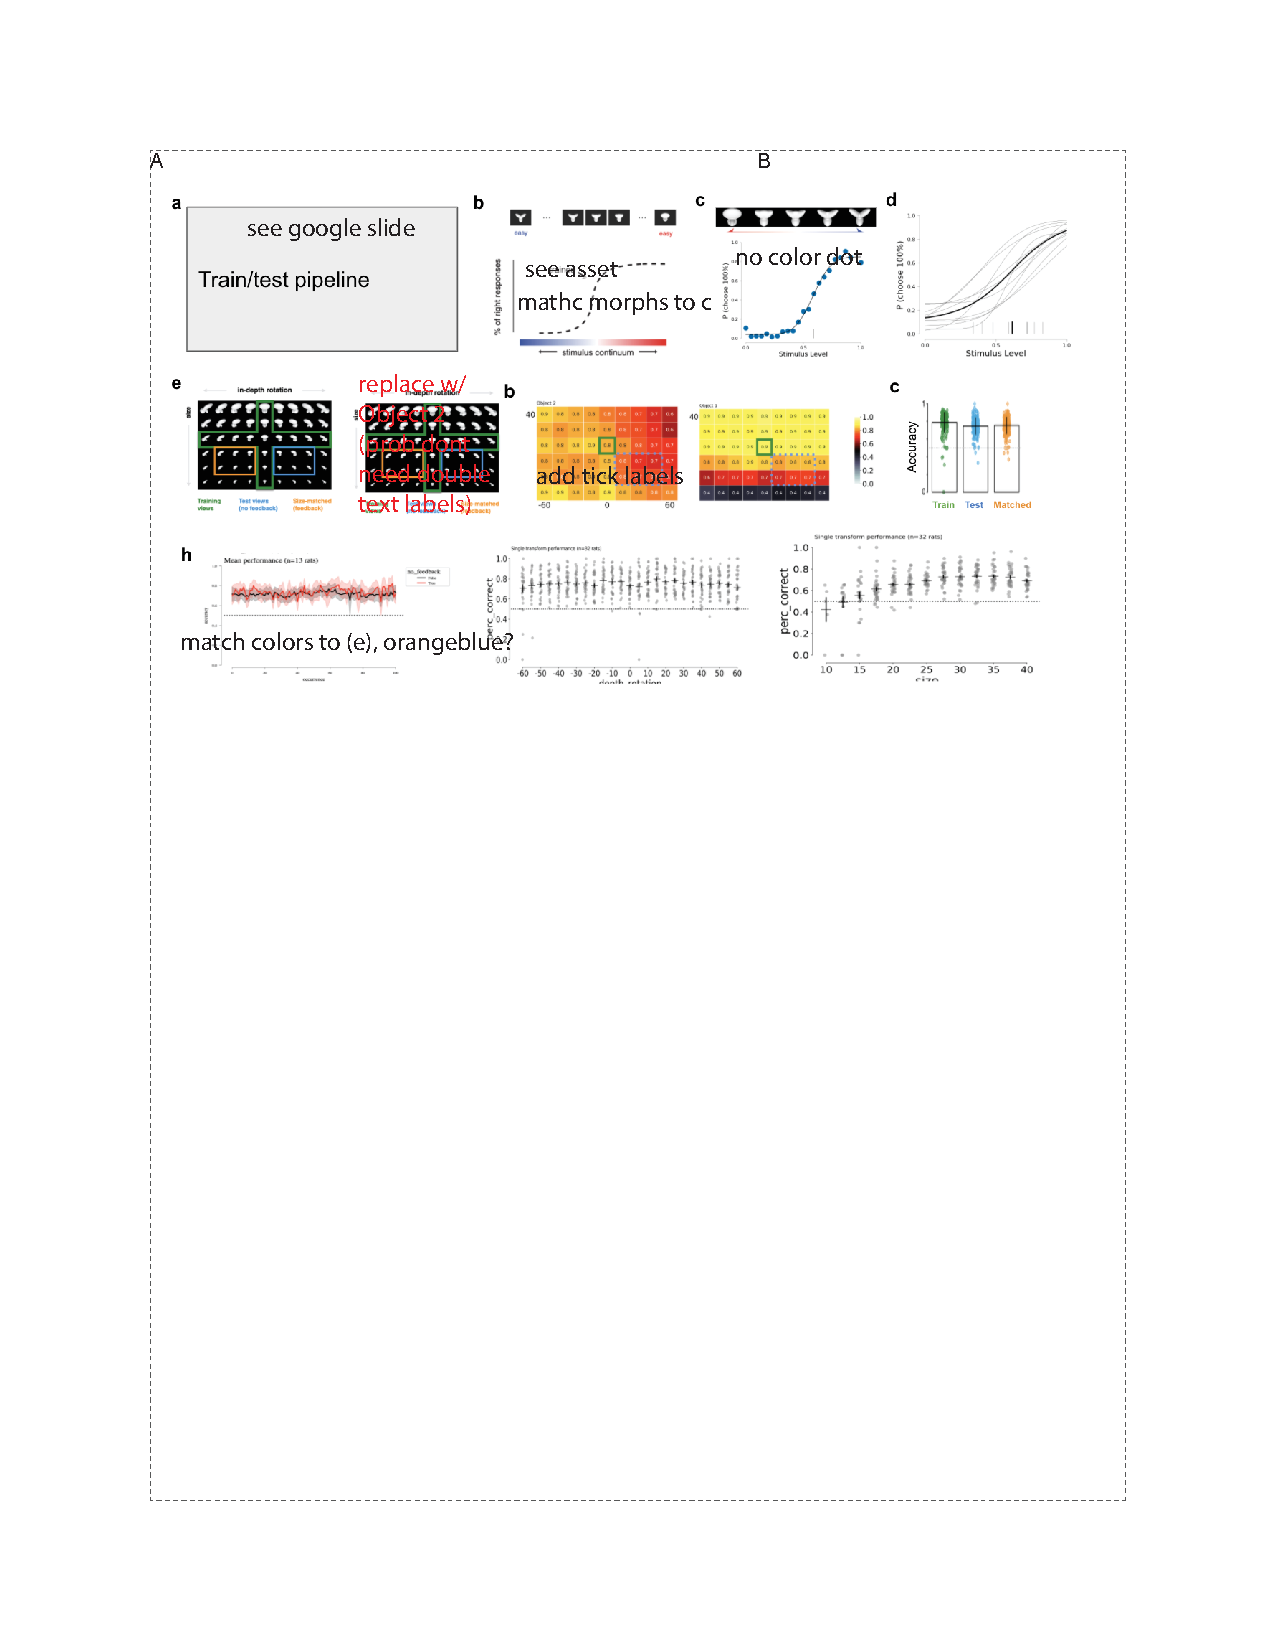
\includegraphics[width=\textwidth]{figures/chapter_1/fig_1-3_behavior_generalization/fig_1-3_behavior_generalization.pdf}
    \vspace{.1in}
    \caption[Generalization of visual behavior]{Generalization to identity-preserving and identity-changing transformations. 
    \textbf{A.} Training and testing pipeline. Animals are first trained on the basic discrimination task. Those that pass criterion performance are then tested on identity-changing or identity-preserving generalizations on probe trials that are interleaved with the basic task. 
    \textbf{B.} Morph stimuli create an axis along which identity changes across a stimulus continuum between the original anchors, object A and B. 
    \textbf{C.} Example data on the morph probe trials for one rat. Dots, average across trials for each morph level. Line, fit psychometric curve. 
    \textbf{D.} Pyschometric curves for one cohort (N=10 rats). Thin lines, individual rats. Thick line, average psychometric curve across rats. 
    \textbf{E.} Identity-preserving transformations tested for each of the original objects: 6 sizes and 9 in-depth rotations. Green, subset of conditions used for training. Blue, test transformations for which feedback was never provided. Orange, size-matched, \textit{i.e.}, acuity-matched, transformations of the test views, but for which feedback was provided, to compare the effect of feedback on generalization performance. No-feedback quadrants were counterbalanced across animals. 
    \textbf{F.} Performance for all identity-preserving transformations for each object for an example rat. Colors and stimulus conditions are ordered as in \textbf{E}. \textbf{G.} Accuracy for rats in one cohort (n=10 rats) for train views, test views, and size-matched feedback views. Colors as in \textbf{E}. Each circle denotes session accuracies for a given rat, all rats shown. Error bars, SD. 
    \textbf{H.} Accuracy as a function of the Nth presentation of a given transformation for feedback-provided (orange) and no-feedback (blue) conditions. Shading, SD across animals. 
    \textbf{I.} Accuracy for each depth-rotation tested. Each dot is the session accuracy for a given rat. Lines, mean and SD across sessions. 
    \textbf{J.} Same as \textbf{I}, but for each stimulus size tested. 
    \label{fig:behavior_generalization}}
\end{figure}
%     \caption*{\textbf{Figure 2.1} Example figure and tips -- A) Your figure numbers should follow the format of Figure chapter#.figure#. B) Set width equal to textwidth. C) Specify position as [t!] to insert at page top.}
% \end{figure}

Rats were presented with a morph image on a small fraction of trials (<15\%, see Methods) during the ordinary discrimination task. No feedback was provided on these probe trials in order to measure perceived, rather than trained, perceptual judgements. These probe trials were then used to build up a psychophysical curve to determine the animals' naive behavior in classifying the objects as ``A'' or ``B''. We fit a psychometric curve to the probe trials using maximum likelihood estimation (psignifit4, see Methods). These curves characterize the category boundary along the morph axis. We found that that rats perceptual choices matched the physical similarity of the morphed objects, though there was individual variation across rats (slope, REFREF +/- ; threshold, REFREF +/- SEM; lapse rate, REFREF +/- SEM, across n=10 rats). 

% FIGURE 1.3 INVARIANCE TEST
To test how well animals discriminate objects across shape changes that preserve object identity, we tested the same rats on an object recognition task. Consistent with previous studies\cite{Zoccolan2009, Tafazoli2012Transformation-TolerantPriming, REFREF}, we found that performance generalized robustly across identity-preserving transformations, such as changes in size and in-depth rotation (Figure\ref{fig:behavior_generalization}E). Importantly, accuracy was high on test trials (~80\% accuracy), where animals never received feedback (Figure\ref{fig:behavior_generalization}F-G), demonstrating that performance on novel views was spontaneous, rather than learned. In fact, accuracy was high across all presentations of novel views, with or without feedback (Figure\ref{fig:behavior_generalization}H). Although there was variatiability across animals in accuracy for each of the transformation axes of rotation and size (Figure\ref{fig:behavior_generalization}I-J), all rats showed high accuracy across all views. The only except in the results presented here was low accuracies for the smallest stimulus sizes (Figure\ref{fig:behavior_generalization}J). However, when we tested a separate cohort of animals (not shown) that were only presented with the smallest stimulus sizes, rats showed high levels of performance, suggesting this is a strategy effect, rather than a reflection of rats' inability to perform the task\cite{Masis2020}. These results demonstrate that rats are capable of true generalization, and are not simply learning stimulus-response pairings. 

% ---------------------------------------------------------
% Closing remarks
% \section{Discussion?}
High-throughput behavior is important for practical reasons, but also scientific ones. 
Standardization is important. 

We found that rats readily perform hundreds of trials per day in our behavior system and learn difficult visual tasks in 2-3 weeks. We use OpenRatBox to show that rats robustly generalize to novel views of objects, i.e., across identity-preserving transformations, and make perceptual choices that follow our morph axis of identity transformations. While similar behavioral results have been shown previously\cite{Zoccolan2009, Tafazoli2012Transformation-TolerantPriming, Vermaercke2012}, here, we demonstrate that a) we can replicate these results with our high-throughput behavior system, and b) in response to our particular stimuli, rats respond correctly in the absence of training on the transformations (no feedback conditions and morph probe trials). We will use the same stimuli when characterizing neural representations in naive rats in a later chapter. 

% In Go/No-Go (GNG) paradigms, the animal responds to a given stimulus (the "Go" condition) by licking a choice port or pressing a lever, and must withhold a response otherwise (the "No-Go" condition). GNG paradigms have fewer moving parts, requiring only one response type, which can make it easier to learn. However, subjects tend to make more Go responses in the GNG task, as the Go response is rewarded while other other behaviors are not\cite{REFREF}. 

% For physiology experiments, GNG paradigms are more amenable to head-restrained animals, since the animal only needs to make one type of response. On the other hand, since reward strongly modulates neural activity, and GNG paradigms can be challenging as the stimulus, response, and reward are tightly linked\cite{REFREF}. Multi-port tasks, like two-choice paradigms, overcome many of these drawbacks, as the animal is trained to respond in one way to condition A and some other way to condition B. In this way, the stimulus, response, and reward can be disentangled, but at the cost of a more complicated task structure that can make interpretations difficult in still other ways. However, they can be more difficult to adapt for head-restrained conditions. Animals normally use head movements or their whole body to reach one reward port or the other\cite{REFREF}, which is not possible in physiology experiments that require the animal's head to be fixed in place in the recording apparatus. 


% \texttt{This is a line of code.}


% For an example of a full page figure, see Fig.~\ref{fig:myFullPageFigure}.

% % EXAMPLE FIGURE 
% \begin{figure}[t!]
%     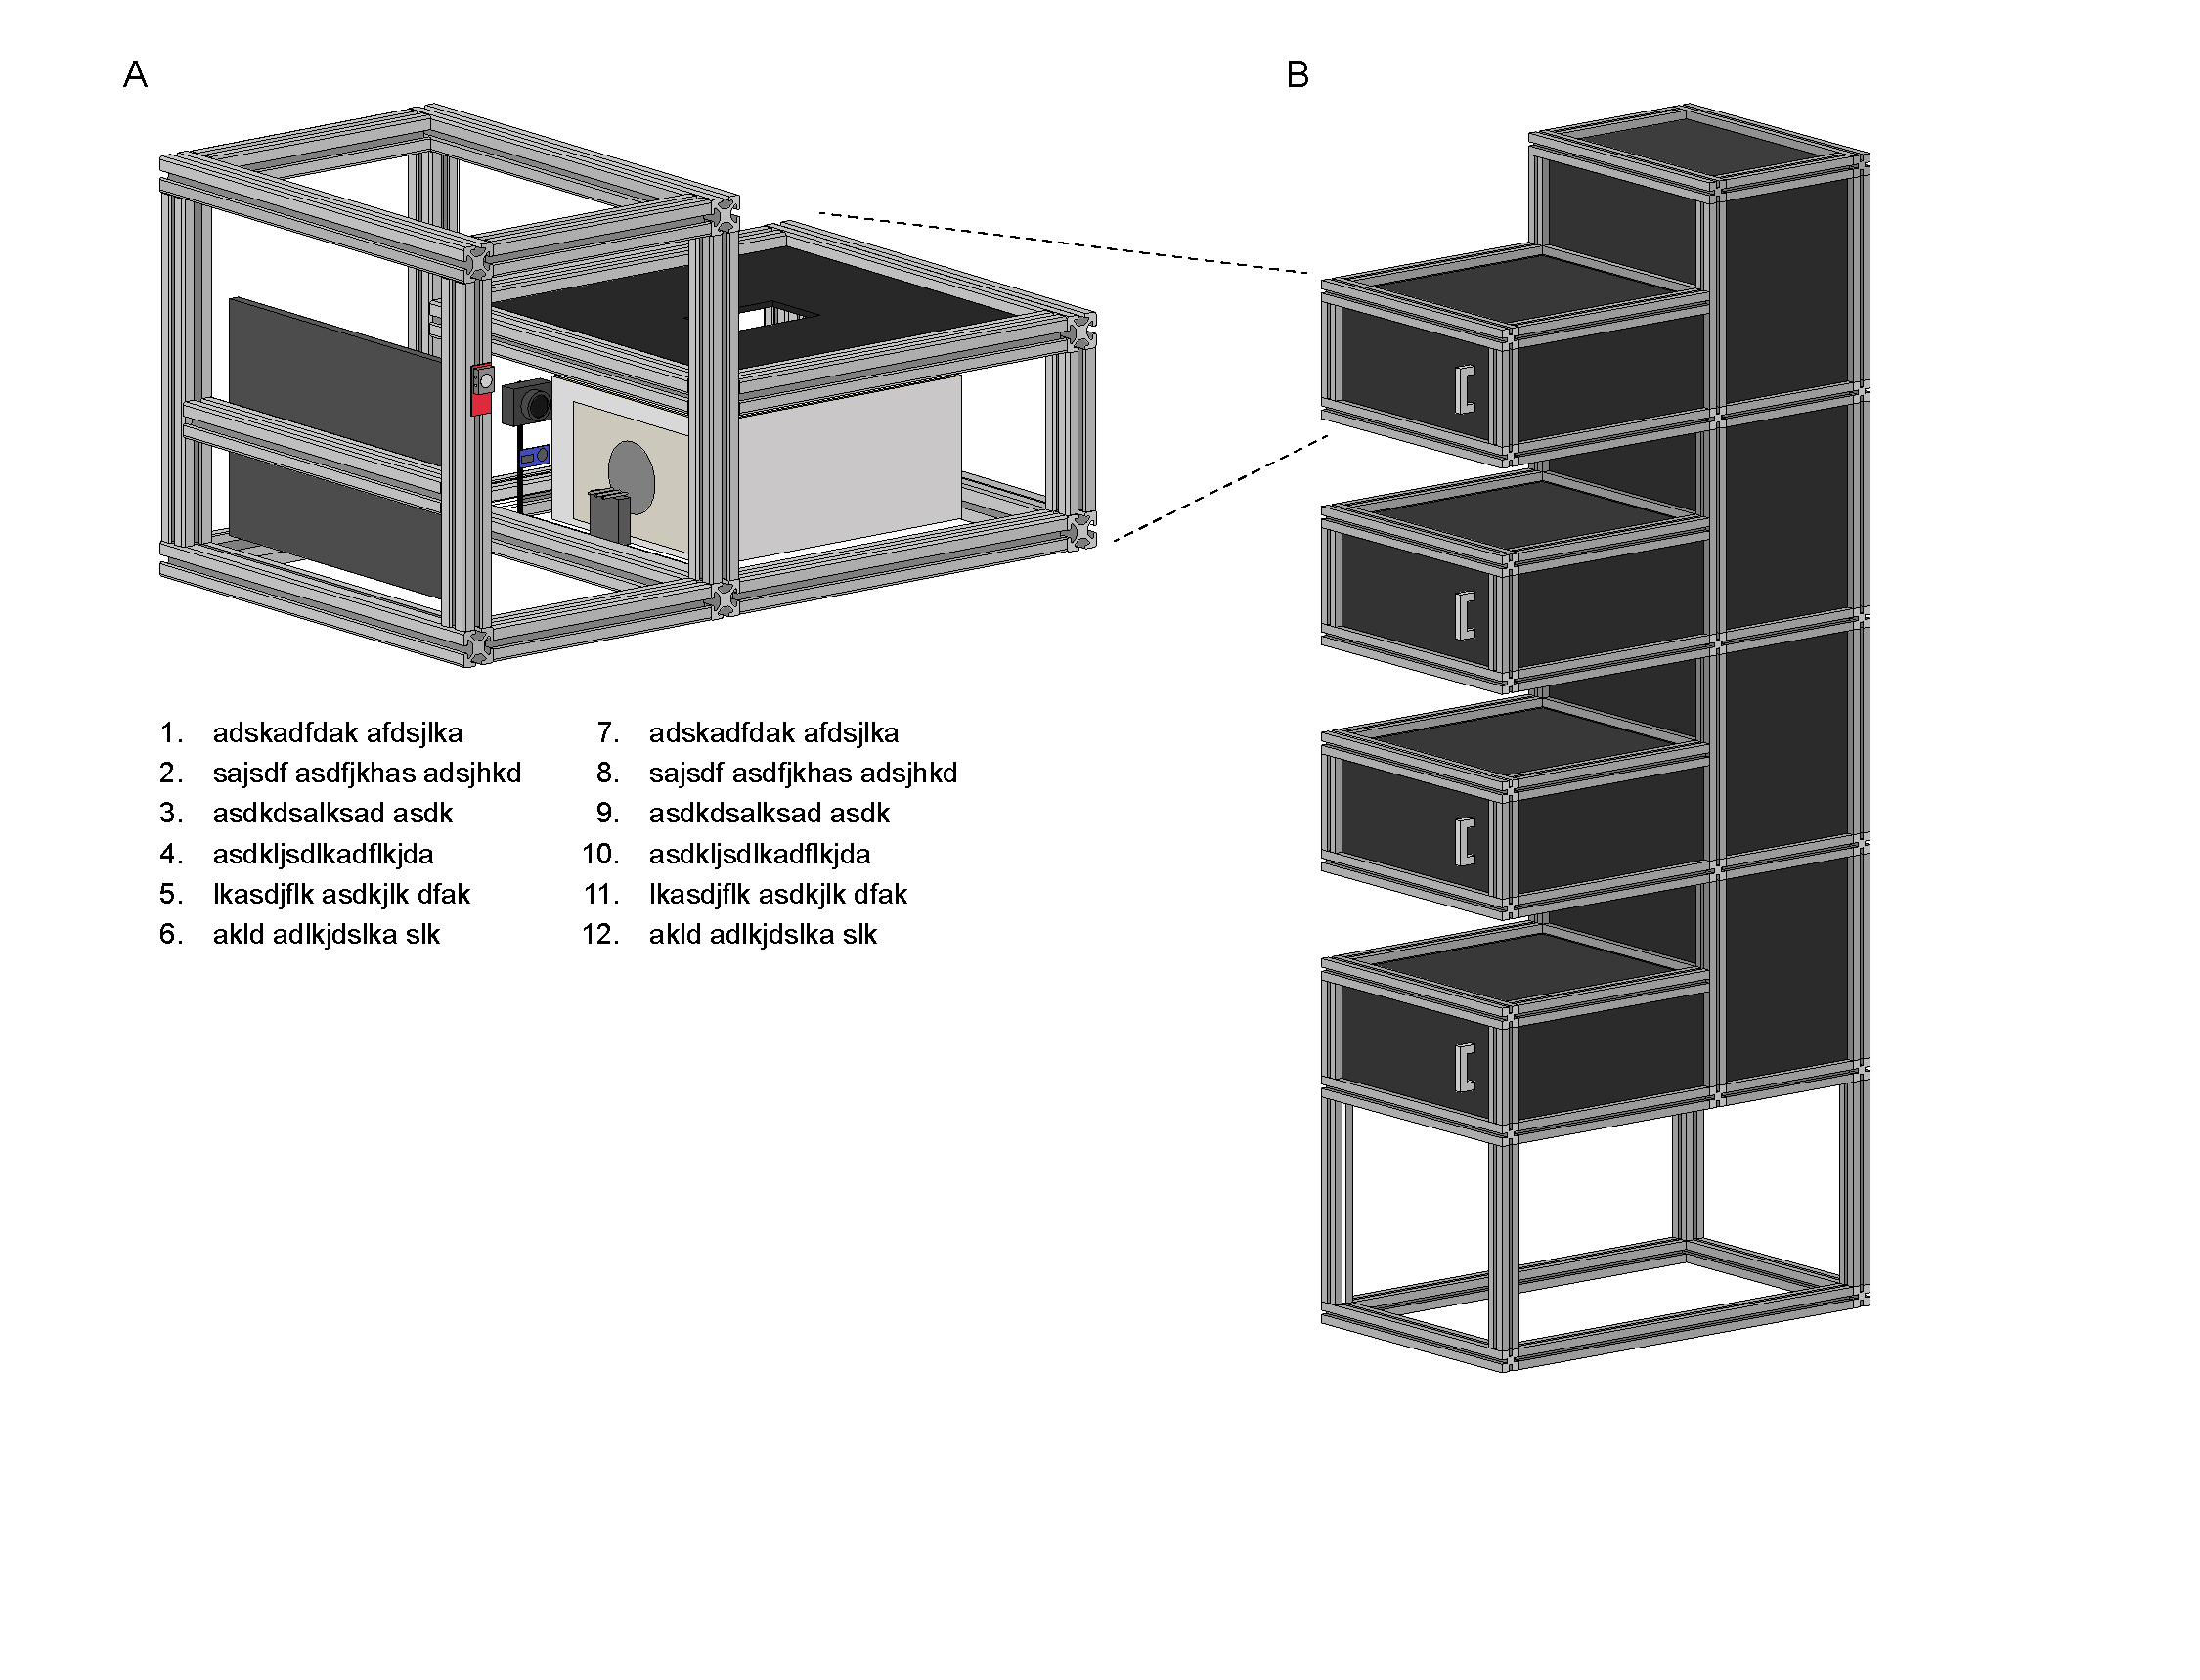
\includegraphics[width=\textwidth]{figures/chapter_1/ratbox_schematic.pdf}
%     \vspace{.1in}
%     \caption*{\textbf{Figure 2.1} Example figure and tips -- A) Your figure numbers should follow the format of Figure chapter#.figure#. B) Set width equal to textwidth. C) Specify position as [t!] to insert at page top.}
% \end{figure}

%% Requires fltpage2 package
%%
% \begin{FPfigure}
% 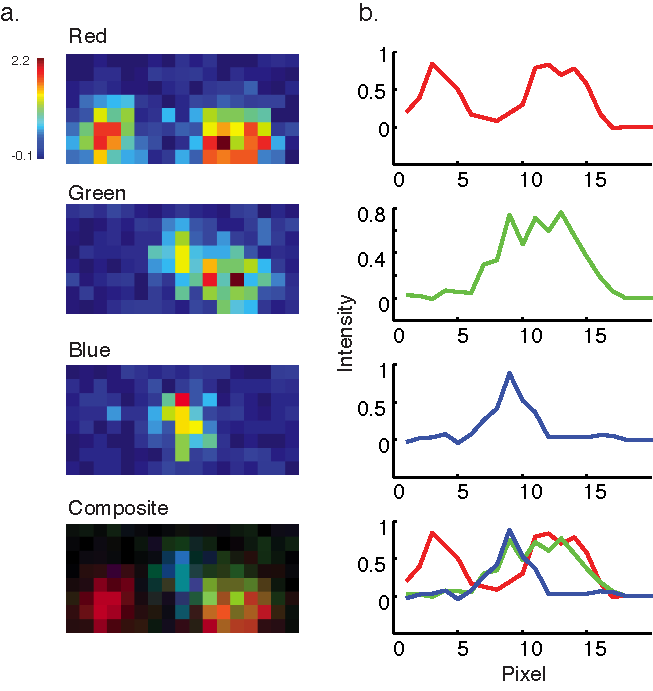
\includegraphics[width=\textwidth]{figures/fullpage}
% \caption[Short figure name.]{This is a full page figure using the FPfigure command. It takes up the whole page and the caption appears on the preceding page. Its useful for large figures. Harvard's rules about full page figures are tricky, but you don't have to worry about it because we took care of it for you. For example, the full figure is supposed to have a title in the same style as the caption but without the actual caption. The caption is supposed to appear alone on the preceding page with no other text. You do't have to worry about any of that. We have modified the fltpage package to make it work. This is a lengthy caption and it clearly would not fit on the same page as the figure. Note that you should only use the FPfigure command in instances where the figure really is too large. If the figure is small enough to fit by the caption than it does not produce the desired effect. Good luck with your thesis. I have to keep writing this to make the caption really long. LaTex is a lot of fun. You will enjoy working with it. Good luck on your post doctoral life! I am looking forward to mine. \label{fig:myFullPageFigure}}
% \end{FPfigure}
% \afterpage{\clearpage}


% \begin{savequote}[75mm]
% OMG... Is that a neuron??
% \qauthor{An Excited Grad Student}
% \end{savequote}

% Ephys:
% (Jun et al., 2017 (neuropixels); 
% Siegle et al., 2019 (hierarhcy, Nature)
% Stringer et al., 2019a -- spontaneous bebaviors, Science

% ca imaging: 
% (Sofroniew et al., 2016; -- meoscope, elife
% Stringer et al., 2019b --high-dim geometry, Nature
% Weisenburger et al., 2019). --- alipasha, Cell

\chapter{Engineering systems for optical imaging in rats}
% INTRO
\newthought{Large-scale recordings} of hundreds and even thousands of neurons are becoming increasingly standard using electrophysiology \cite{Steinmetz2019, Siegle2021, Stringer2019SpontaneousActivity} and optical imaging \cite{Stringer2019High-dimensionalCortex, Weisenburger2019, Sofroniew2016}. With rapid advancements in genetic tools, hardware design, and computational power, we are in an unprecedented and exciting time to be studying neural circuits and behavior. For measuring neural populations in an awake animal, there are two main classes of methods: imaging and electrophysiology. Both are extremely powerful, and choosing one or the other is highly dependent on the goals of the experiment. 

Electrophysiology provides the most direct access to neural activity, as it measures voltage changes with high temporal resolution, allowing for measurements of single spikes and sub-threshold activity. It is also amenable to tethered or even wireless systems that allow animals to move about relatively freely, thus allowing a more naturalistic setting for studying neural circuits and behavior in the lab. However, long-term access to a given neuron and the throughput of how many neurons can be recorded simultaneously is limited by the uncertainties in single unit isolation, the capacities of electronic components, and how many channels one can physically fit and successfully record from in a small animal. 

In contrast, optical imaging approaches allow the same cells to be tracked for long periods of time, and simultaneous recording of large populations (hundreds to thousands) in the same animal. Optical imaging of neural activity relies on genetic tools that enable fluorescent indicators to be expressed in targeted cell populations. Standard approaches rely on tracking changes in calcium activity that occur in response to voltage changes in a neuron, usually by measuring fluorescent changes in genetically-encoded fluorescent calcium indicators (GECIs)\cite{Akerboom2012, Chen2013UltrasensitiveActivity}, which fluoresce in response to calcium binding. As such, the measured signal is slower and not a direct readout of neural activity, as measured by electrophysiology. In transgenic animals, GECIs can be expressed in a controlled manner, from sparse labeling\cite{Dana2014} to pan-neuronal expression\cite{Daigle2018}. In the absence of a transgenic animal or in combination with one that expresses a different gene of interest, one can also use viral vectors, such as an adeno-associated virus (AAV) or lentivirus, for robust delivery of the GCaMP construct, and expression of the indicator remains robust and stable over at least several months.

Physical access to deep or lateral parts of the brain is limited with optical methods, which typically rely on imaging the brain from directly above the animal's head. Many optical systems are bulky, making it quite difficult to record from freely moving animals. While electrodes can be inserted deep and at any angle into the brain, optical access to deeper brain structures sometimes requires removing superficial layers, or using mirrors to direct the light path in clever ways while keeping the collection system above the animal\cite{Andermann2013}. Head-mounted optical systems allow for cellular resolution imaging in freely moving animals\cite{Helmchen2001, Sawinski2009, Zong2017}, and high-photon-count imaging, \textit{e.g.}, >3 photon\cite{Klioutchnikov2020}, improve optical access to deeper brain structures.

However, the gap between the two methods continues to get smaller, as technological advancements offer improvements to the challenges each face. There continue to be major technical advances in electrophysiological approaches, such as high-density electrode arrays\cite{REFREF} and computational methods for processing high channel count data and verifying chronic access to specific cells\cite{REFREF}. For imaging, each generation of calcium indicators has proved increasingly more powerful, \textit{e.g.}, higher signal-to-noise (SNR), multi-color alternatives, and higher temporal resolution \cite{Akerboom2012OptimizationImaging, Chen2013UltrasensitiveActivity}. Progress has also been made toward developing voltage-sensitive indicators\cite{Bando2019, Villette2019}, which have the potential to combine the advantages of spatial and genetic access provided by optical methods with the more direct signal and higher temporal resolution of electrophysiology.

Today, one of the greatest advantages of optical imaging is cellular resolution access to large swaths of the brain. To be able to visualize single neurons as a population in awake animals is immensely powerful, especially in concert with sophisticated manipulation techniques, such as multi-channel optogenetics \cite{REFREF}, holographic light stimulation \cite{REFREF}, and genetically-defined targeting of specific populations of cells. In combination, these features allow one to measure and manipulate the same neurons in awake, behaving animals across large numbers of stimuli and trials over the course of weeks and months. In contrast, conventional acute single-unit microelectrode recordings are limited by the time that a single cell can be isolated (usually only one or a few hours). Even the best chronic preparations face difficulties holding isolated cells over very long time periods, and it is difficult to be absolutely confident that the same cell is isolated across days, especially given that nearby cells are often thought to have similar response properties.

%% % What has been done, and what's missing  ---------------------------
For cellular resolution imaging, most studies rely on head-fixed preparations in which that animal's head is fixed in place for clear optical access. Multi-photon imaging systems are usually table-top designs, as the equipment is quite bulky and stable imaging planes are needed for quality imaging. Miniature head-mounted two-photon microscopes offer an alternative to head-fixation during in vivo imaging \cite{Helmchen2001, Piyawattanametha2009, Sawinski2009}. Such techniques can be powerful for measuring neural activity in a wide range of naturalistic behaviors \cite{Sawinski2009}, but the technical difficulty of using these miniaturized microscopes has limited their use as a standard tool in neuroscience \cite{Kerr2012}. Furthermore, many other in vivo imaging technologies are difficult to miniaturize, preventing their use as head-mounted devices. 

Studies using head-fixed animals have access to certain experimental advantages, such as restrained movement, precise stimulus control, and longitudinal studies that can track the same neurons over long timescales. While head-fixed preparations are routinely used in flies and mice, rats are much harder to restrain with these protocols, given their larger size and prohibitive movement artifacts for cellular-resolution imaging. As such, most studies using head-fixed rats rely on electrophysiology. Furthermore, the lateral position of many brain areas of interest in the rat (see Introduction) makes optical access all the more challenging, and most rat imaging studies have been restricted to primary visual cortex, V1\cite{Greenberg2008, Ohki2005, Scott2018}.

Although a large body of scientific research relies on the rich behavioral repertoire of rats, it has not been possible to fully leverage recent developments in optical imaging and molecular and genetic tools, as has been done with great success in smaller animals like mice. In one heroic study, Scott \textit{et al.} developed a method for training rats to voluntarily head-fix themselves into a two-photon system, which allowed for cellular resolution imaging in awake, behaving rats \cite{Scott2013}. However, voluntary head-fixation can be difficult and time-intensive, and if successful for a given rat, still places significant limitations on how much control the experimenter can have over the time course of the study. More recently, the same group also created a transgenic rat expressing GCaMP in all neurons, and demonstrated the feasibility of recording population dynamics in awake, freely moving rats, albeit without cellular resolution\cite{Scott2018ImagingMacroscope}. 

% FIGURE 2.1 Rat visual areas
\begin{figure}[t!]
    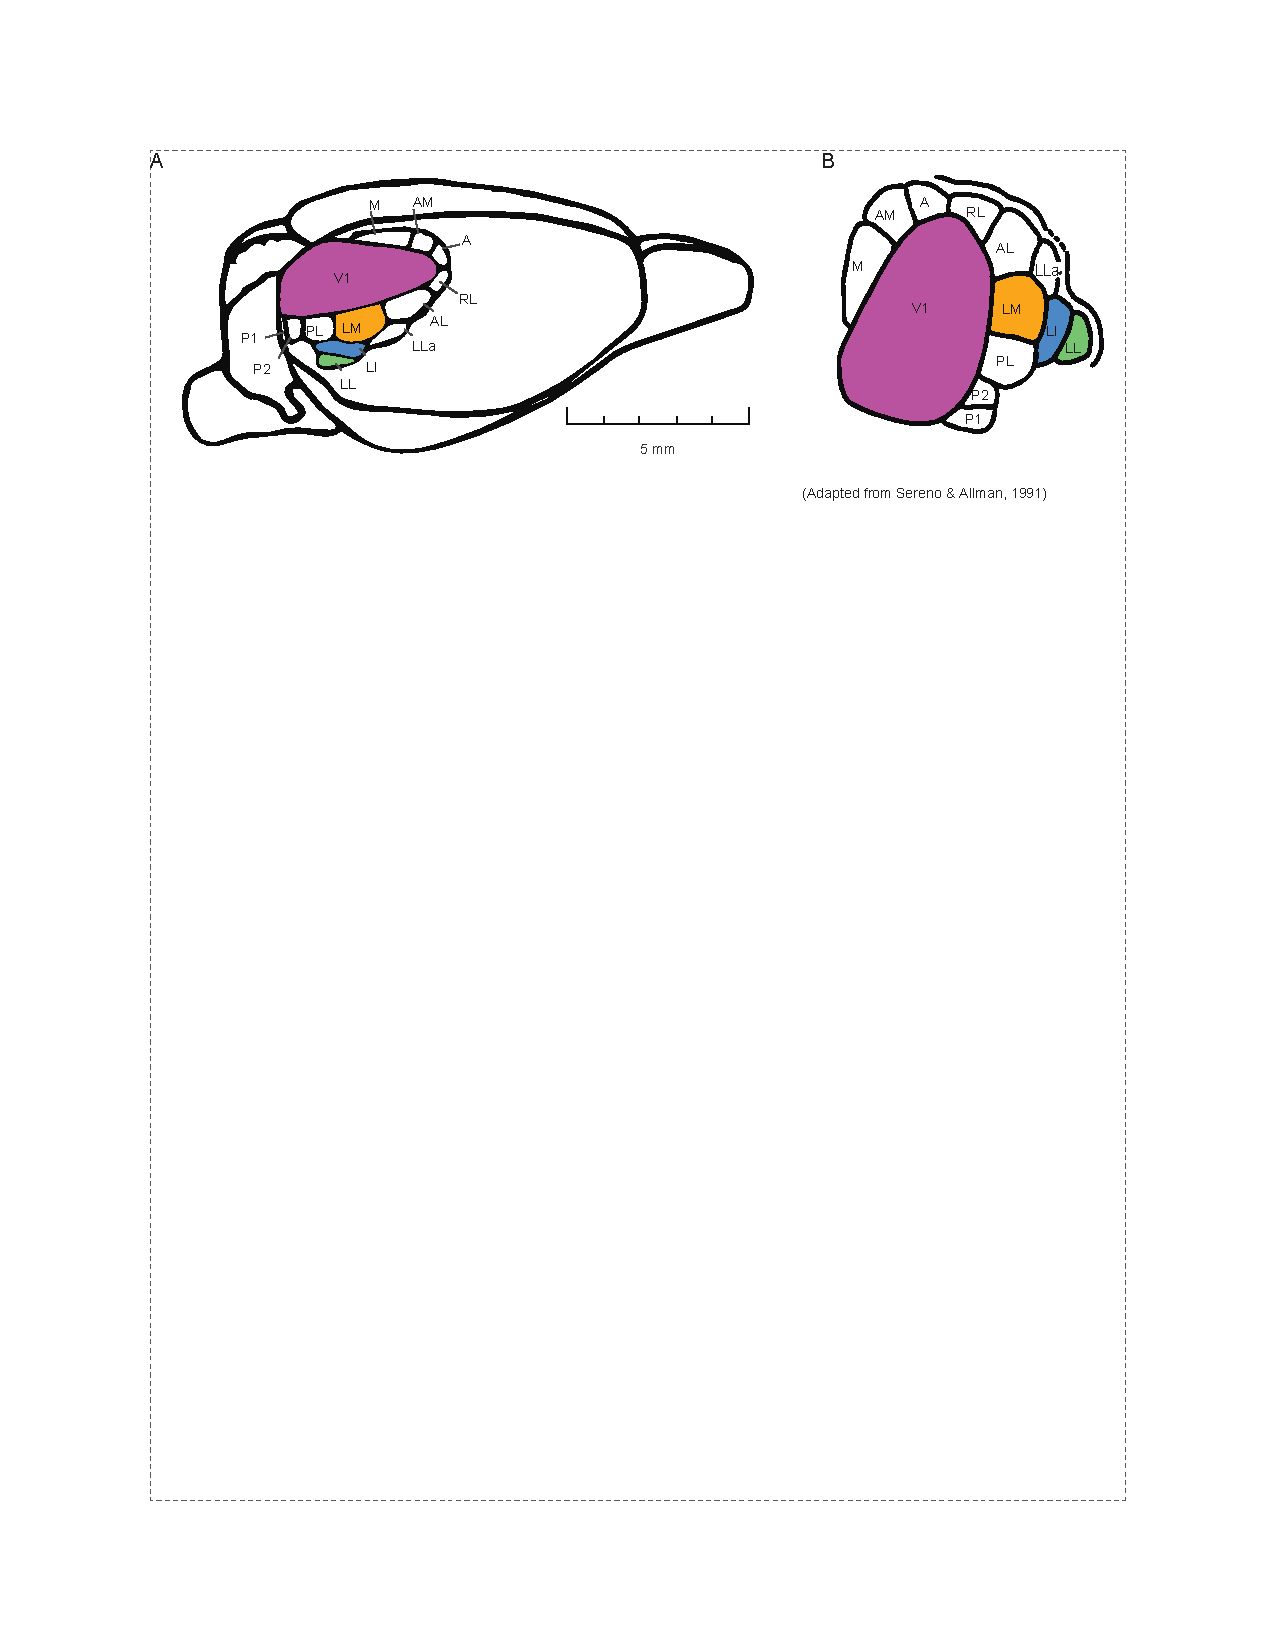
\includegraphics[width=\textwidth]{figures/chapter_2/fig_2-1_rat_visual_areas/fig_2-1_rat_visual_areas.pdf}
    \vspace{.1in}
    \caption[Visual areas in the rat]{Visual areas in the rat (adapted from \cite{Sereno1991}). 
    \textbf{A.} Lateral view of visually responsive areas identified by electrophysiological mapping of retinotopic preference. 
    \textbf{B.} Flattened representation of lateral visual areas, with targets of the present study, areas V1, LM, and LI, highlighted in color. 
    \label{fig:rat_visual_areas}}
\end{figure}

Almost all of our knowledge about rat visual cortex comes from electrophysiology studies. To date, the only area of visual cortex to be imaged from in rats is primary visual cortex, or V1, from intrinsic signal \cite{Gias2004} to single-photon \cite{Scott2018ImagingMacroscope} and two-photon \cite{Ohki2005, Greenberg2008} imaging. However, rat visual cortex contains several areas, the largest of which is striate or primary visual cortex, or V1, with additional extrastriate areas surround V1 \cite{Espinoza1983RetinotopicRat, Sereno1991} (Figure~\ref{fig:rat_visual_areas}). In rats, areas V1, LM, LI, and LL lie along the medial-to-lateral axis at the posterior edge of the brain, extending well beyond the lateral bone ridge. These visual areas have gained significant interest within the last ten years, as neurons in these areas, as measured by electrophysiology, appear to have several functional similarities to those characterized along the ventral stream of the primate brain (see Introduction). With genetic tools becoming increasingly available in rats, there is immense potential for a head-fixed system in which many of these tools can be fully leveraged. We developed a method for cellular-resolution imaging of large FOVs in awake, head-fixed rats with the ultimate goal of chronic cellular resolution access to the visual cortex of rats. 

Optical imaging approaches allow the same field-of-view (FOV), and with multiphoton imaging, the same cells, to be imaged across multiple sessions. Our approach aimed to combine head-fixation in awake rats, optical access to multiple brain areas, and precise re-positioning for long-term studies of chronically implanted animals. Several major challenges we needed to address were:  1) implant stability against the significant mechanical forces that awake rats are able to apply, 2) motion artefacts due to large displacements in moving rats, and 3) accessibility of large FOVs over the extreme, lateral edge of the rat skull.


\section{Procedures for optical access and long-term viability} 
% %%%%%%%%%%%%%%%%%%%%%%%%%%%%%%%%%%%%%%%%%%%%%%%%%%%%%%%%%%%%%%%%
% Surgery + implant
% %%%%%%%%%%%%%%%%%%%%%%%%%%%%%%%%%%%%%%%%%%%%%%%%%%%%%%%%%%%%%%%%
% fig:experimental_pipeline
% fig:surgery_steps
% fig:headplate_schematic
% fig:retino_mapping
% fig:2p_schematic
%fig:multiday_imaging

% Figure: Experimental workflow
\begin{figure}[t!]
    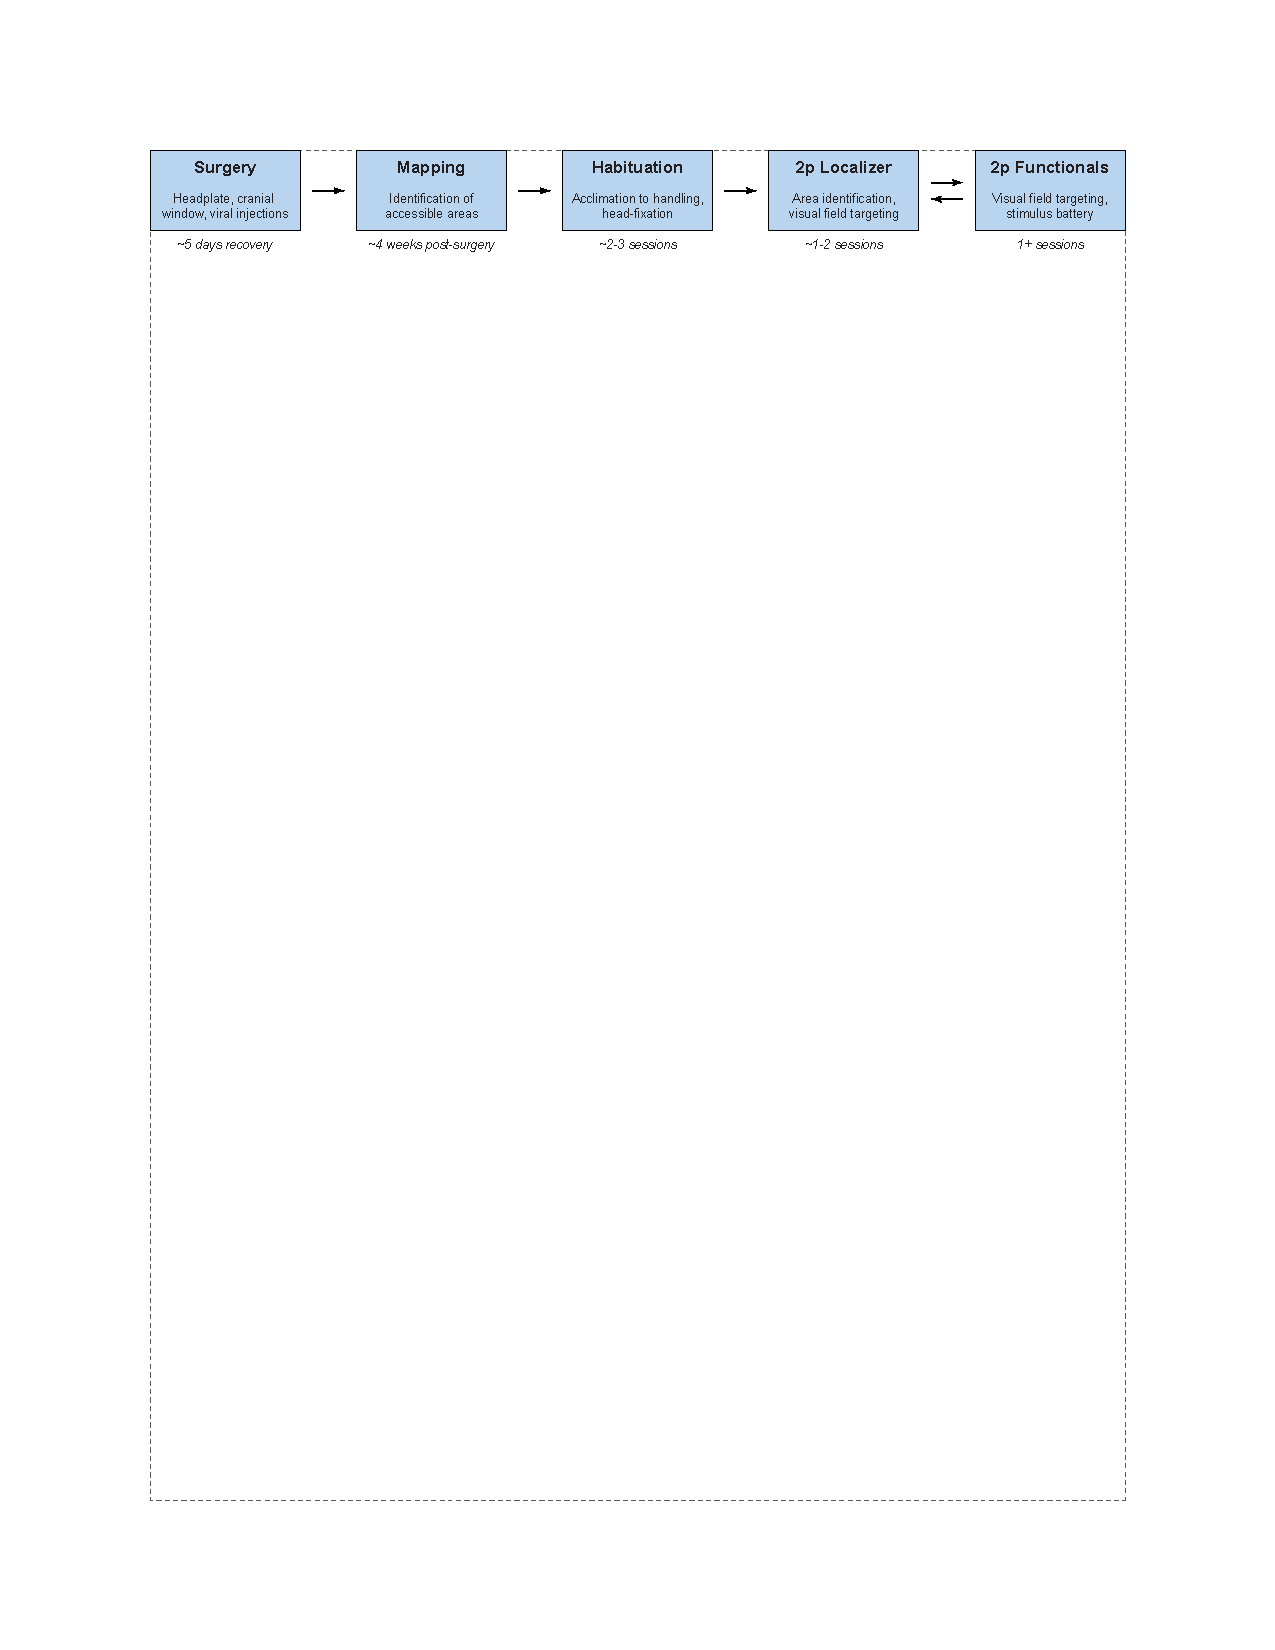
\includegraphics[width=\textwidth]{figures/chapter_2/fig_2-2_experiment_workflow/fig_2-2_experiment_workflow.pdf}
    \vspace{.1in}
    \caption[Experiment workflow]{Experiment workflow. 
    \textit{Surgery:} Animals first undergo chronic implant and cranial window surgery. Viral delivery of the calcium indicator is done during this surgery, as $\sim$4 weeks are needed for expression to come online throughout the window.
    \textit{Mapping:} Once most of the window exhibits fluorescence, the mapping procedure identifies which visual areas are identifiable and accessible within the extent of the window. Viable cranial windows must meet several criteria for animals to continue through to the next stage: sufficient expression, identifiable visual areas, and any of the three areas of interest (V1, LM, or LI/LL). \textit{Habituation:} These animals are then habituated over several days in preparation for two-photon imaging. After habituation, candidate imaging sites, or fields-of-view (FOVs), are selected for two-photon characterization. \textit{Localizer:} Candidate FOVs are then imaged to validate visual area assignment via retinotopic preference and gradient (see Methods), to target stimulus locations in the visual field based on the receptive field positions of the cells in the FOV. 
    \textit{Functionals:} Vetted FOVs are characterized with a battery of visual stimuli. Localizer runs are also repeated during functional sessions. 
    \label{fig:experiment_workflow}}
\end{figure}

% Habituation + shaping
For many behaviors of interest, it is not possible to use sedatives or other anesthetics during neural recording. This is particularly true for paradigms that rely on animals performing a task or engaging in a behavior. However, not only is it difficult to acquire quality cellular resolution recordings in struggling animals, but moreover, stress has been shown to negatively impact learning rates\cite{REFREF}. Thus, it was critical to establish an experimental workflow that led to a visibly calm rat, even while head-fixed for long periods of time. We developed an extensive pipeline of surgical and experimental procedures for large-scale visual characterizations in awake, head-fixed rats (Figure\ref{fig:experiment_workflow}). Rats are much larger than mice, so a key challenge was to prevent awake rats from ripping themselves out of their implants and keeping the FOV stable enough for cellular resolution imaging. 

% window surgery --------------------------------------
%\subsection{Cranial windows for chronic imaging in awake rats}
Since chronic cranial windows are almost routine procedures in mice, we first adapted a mouse surgical protocol\cite{Goldey2014} and optimized it for rats, with a focus on strong implant adhesion and long-term viability, even against the significant forces that awake rats can apply (see Methods). For calcium imaging, we relied on viral expression of GCaMP\cite{Dana2019High-performanceMicrocompartments} across an area of cortex covering about 4-6mm. A region of this size was large enough to contain multiple visual areas in the rat, based on known cortical extents of extrastriate areas (see Figure\ref{fig:rat_visual_areas}). Since the transgenic GCaMP rat \cite{Scott2018} had not been developed yet, it was important to calibrate the correct volume, titre, and injection method for consistent, widespread expression of the virus throughout the window (see Methods). Finally, since it is not possible to image through a thinned skull or a dura, as it is in mice, we also optimized methods for successful durotomies in the rat (Figure\ref{fig:surgery_steps}). 

% Figure: Cranial window + implant
\begin{figure}[t!]
    \includegraphics[width=\textwidth]{figures/chapter_2/fig_2-3_surgery_steps/fig_2-3_surgery_steps.pdf}
    \vspace{.1in}
    \caption[Chronic cranial window]{Implant of chronic cranial windows for GCaMP imaging. 
    \textbf{A.} Exposed cortical surface after craniotomy and durotomy during a microinjection of AAV-GCaMP. Blue, dye used to visualize spread (see Methods) \textbf{B.} Bright-field view of a cranial window. 
    \textbf{C.} Fluorescent view of GCaMP expression in a cranial window.
    \label{fig:surgery_steps}}
\end{figure}

There were several possible points of attrition before a rat became viable for imaging. In our hands, viral expression was best starting at ~4 weeks post-injection. We tried various combinations of surgical steps to optimize this time-window --- for example, starting with large viral injections through a burr hole near the site of the cranial window, then waiting four weeks before exposing the cortical surface with a craniotomy-durotomy procedure and placing the coverslip window. However, for long-term window viability and high-quality imaging, we found the most reliable approach was to combine the implant surgery and the cranial window with viral injections as close in time as possible, preferably in the same surgery. When splitting the surgical steps, waiting too long (\textit{i.e.}, a week or more) compromised the structure of the skull bone, making window placement unstable and window "clouding" (growth of tissue or an inflammatory response within the cranial window that precludes imaging) much more likely. 

% Figure: Headplate and holding the rat
\begin{figure}
    \includegraphics[width=\textwidth]{figures/chapter_2/fig_2-4_headplate_schematic/fig_2-4_headplate_schematic.pdf}
    \vspace{.1in}
    \caption[Headplate design and assembly]{Headplate design and assembly. \textbf{A.} Schematic showing the assembly for head-fixing the animal. A thick, custom-cut steel post is affixed to the platform (modular design for both habituation setups and imaging setups). An angled bracket, custom-cut to match the desired angle of the objective, contains 3 grooves that hold spherical ceramic balls (close-up, \textit{right}), which mate with the titanium headplate. \textbf{B.} Schematic of a rat skull with a custom titanium headplate positioned over the approximate location targeted for lateral extrastriate areas in the rat. Circle and inset indicate the position of the optical window implanted over these areas. A photograph of the cortical surface accessible for imaging beneath the 5-mm diameter optical window is shown to the right for illustration. 
    \label{fig:headplate_schematic}}
\end{figure}

% Headplate assembly
In order to access lateral visual areas while keeping the rat’s head and body in a relatively natural resting position, our approach was to tilt the imaging plane relative to the animal’s head. This meant implanting the headplate at an angle that matched that of the objective. We leveraged the high precision afforded by kinematic mounts to design custom titanium headplates that could be mounted at steep angles while preserving the capacity for precise re-positioning (Figure\ref{fig:headplate_schematic}). The headplates contained three semi-spherical grooves that mated with stainless steel ball bearings mounted to an aluminum post on the imaging platform. The headplate mated with a steel post designed to be strong enough to hold the animal stably, while keeping the view to the stimulus monitor unobstructed on one side of the animal, and on the contralateral side, sufficiently clear for the objective. Implanted animals were stably positioned at the farthest angles tested (40-45 degrees, where 0 degrees is parallel to ground, or flat on the skull).  

% %%%%%%%%%%%%%%%%%%%%%%%%%%%%%%%%%%%%%%%%%%%%%%%%%%%%%%%%%%%%%%%%
% Identifing visual areas
% %%%%%%%%%%%%%%%%%%%%%%%%%%%%%%%%%%%%%%%%%%%%%%%%%%%%%%%%%%%%%%%%
\section{Functional identification of visual areas}
% Figure: WF retino_mapping/area segmentation
Visual areas are retinotopically arranged --- each area contains a representation of the visual field called a retinotopic map, where nearby positions in physical space are represented by nearby cells on the retina, and this spatial arrangement is preserved from one part of the visual system to the next\cite{REFREF}. Conveniently, nearby visual areas have predictable ``reflections'' of retinotopic space at area boundaries. As such, distinct visual areas can be functionally identified by these mirror reflections in the representation of the visual field. To date, though several methods have been used to image neural activity in rat cortex, from intrinsic signal\cite{Gias2004} to single-photon \cite{Scott2018ImagingMacroscope} and two-photon \cite{Ohki2005, Greenberg2008} imaging, the primary visual cortex, or V1, is the only area of visual cortex yet imaged in rats.

% WIDEFIELD --------------------------------------
\subsection{A tandem-lens macroscope for wide-field imaging}
Our first step was to optically map extrastriate areas of rat visual cortex for the first time. We needed a large field-of-view (FOV) that could capture the full extent of the window (4-5$mm$ diameter). In order to ensure robust mapping with high signal-to-noise, we also needed a sufficiently shallow depth of field for avoiding out-of-focus artefacts (\textit{i.e.}, good axial resolution). To meet these needs, we developed a tilting tandem-lens epifluorescence macroscope\cite{Ratzlaff1991} (Figure\ref{fig:retino_mapping}). 

The macroscope combined two lenses in reverse configuration with a CCD camera, all custom-mounted on a rotating plate with a translating stage --- this allowed us to both rotate the imaging plane about the animal, and gave us manual control for precise positioning with manual micromanipulators. At the start of each session, we captured a high-resolution (656x492, $9.9um$ pixels) image of the surface vasculature beneath the optical window for coregistering two-photon imaging FOVs within the extents of the window. For functional imaging, we focused below the surface to ~$500um$ using micromanipulators.

% Figure:  retino_mapping (WF)
\begin{figure}
    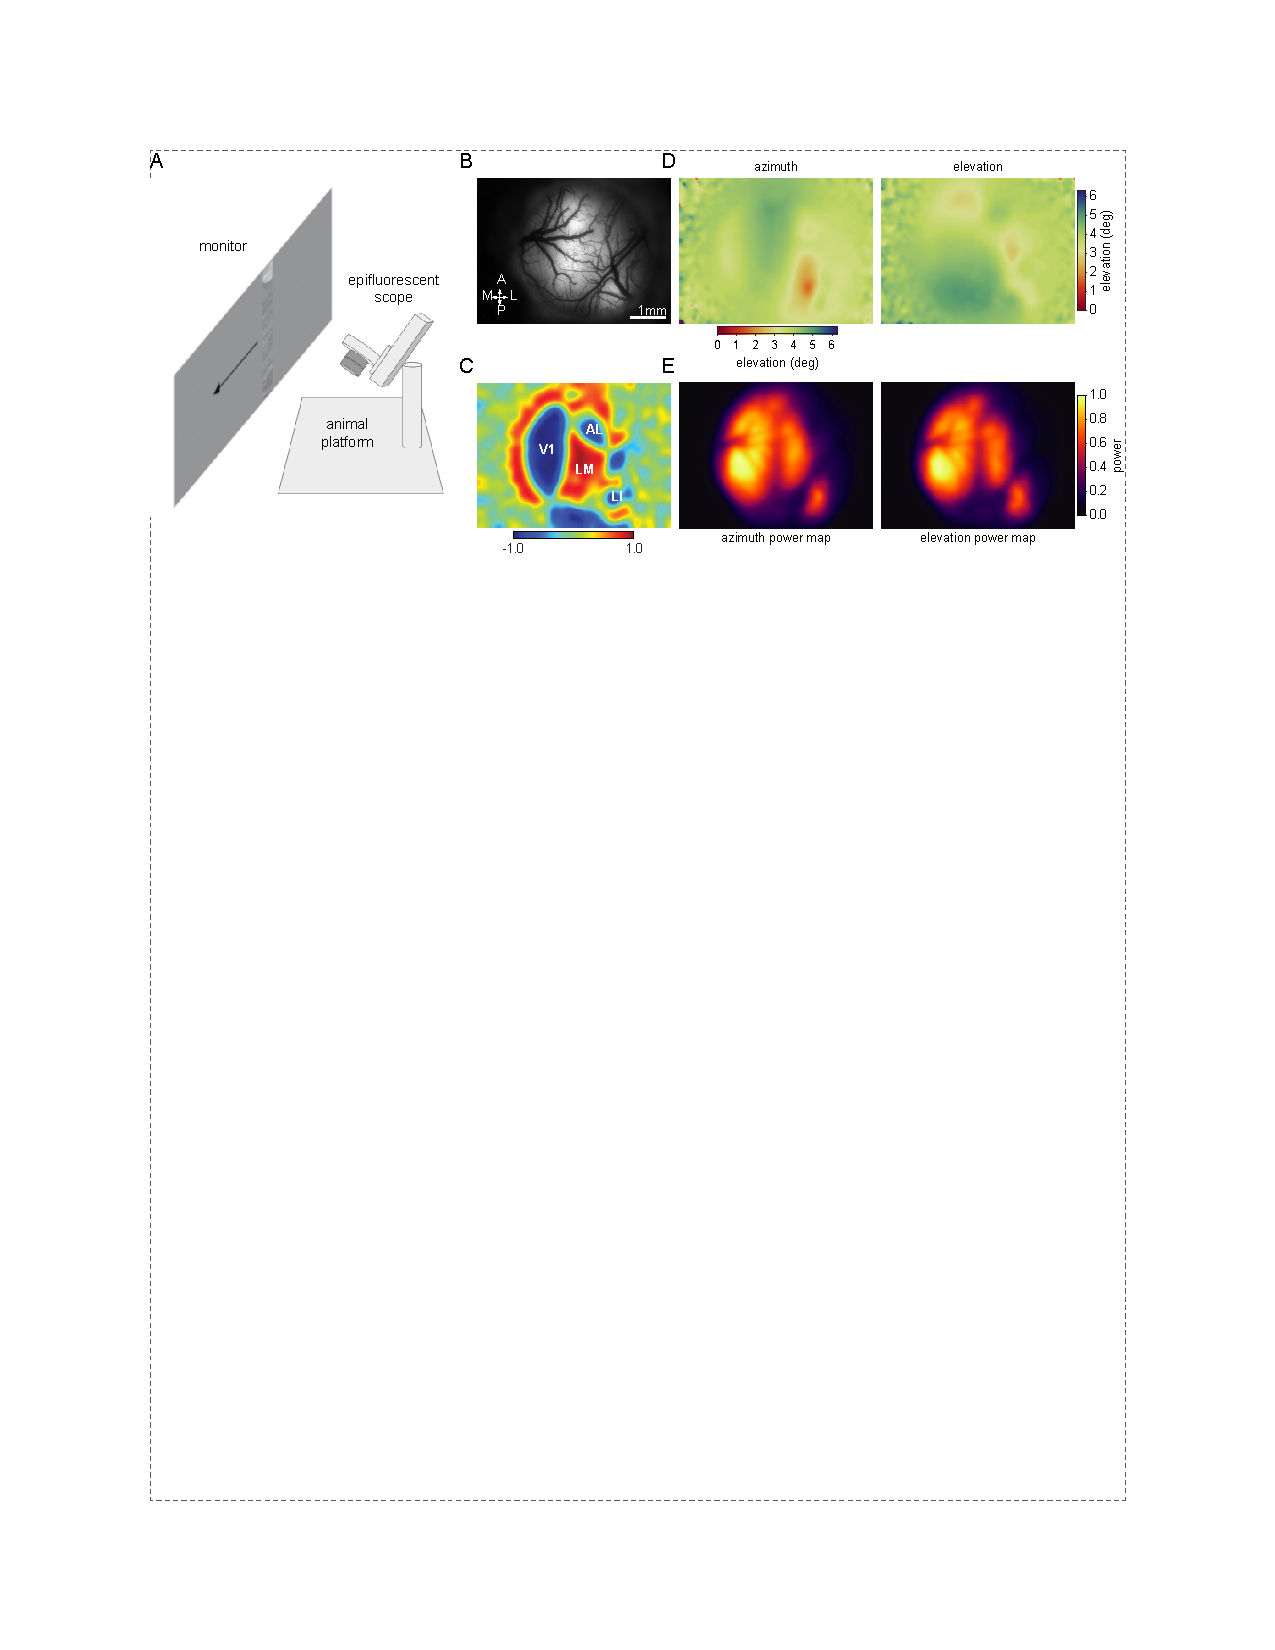
\includegraphics[width=\textwidth]{figures/chapter_2/fig_2-5_retino_mapping/fig_2-5_retino_mapping.pdf}
    \vspace{.1in}
    \caption[Wide-field mapping]{Identifying visual area boundaries. 
    \textbf{A.} Schematic of the tandem-lens macroscope setup used for fast mapping of the entire cranial window. 
    \textbf{B.} Widefield, epifluorescence image of the cranial window. Scale bar, 1mm.
    \textbf{C.} Pseudo-colored image from phase-encoded mapping of retinotopic preference along azimuth (left) and elevation (right). 
    \textbf{D.} Sign map calculate from the gradient of the images in \textbf{C}. \textbf{E.} Normalized power for azimuth (left) and elevation (right) mapping conditions used to threshold area maps. 
    \label{fig:retino_mapping}}
\end{figure}

\subsection{Wide-field functional mapping}
For fast acquisition of retinotopic maps, we used Fourier-based calcium imaging\cite{Kalatsky2003} (Figure\ref{fig:retino_mapping}). This approach is less time-consuming (<10 minutes) than traditional event-based paradigms in which discrete positions on a monitor are stimulated one-by-one across repeated presentations to average over noisy responses, which can take many minutes or longer. In a standard Fourier-based mapping experiment, a moving bar cycles across the screen several times at at particular frequency. The position on the screen to which a given pixel best responds corresponds to a particular part of the bar's cycle, \textit{i.e.}, the phase of response at the stimulation frequency, while how strongly a pixel responds is given by the magnitude of its response at that frequency. Calculating the phase and magnitude of response for each pixel generates a 2D map of phase and magnitude. The phase map is the retinotopic map, which we use to delineate area borders base on the mirror reflections (see Figure\ref{fig:retino_mapping}), and the magnitude map can be used to filter out unresponsive pixels (and thus, remove phase values that are meaningless). 

Visual stimuli were presented using custom Python scripts (see Methods) on a large LCD monitor, which was centered in front of the left eye to span the animal's visual field left visual field (~177$^{\circ}$ of visual angle along azimuth, 67$^{\circ}$ along elevation). The mapping protocol consisted of a periodic, moving bar stimulus\cite{Kalatsky2003, Marshel2011} presented to the (left) eye contralateral to the cranial window. The bar was either a white bar drifting over a black background or an apertured bar containing a random subset of natural scene images drifting over a gray background. We did not find an clear difference between the two bar types, but qualitatively, the latter seemed quite reliable, so we primarily used the natural scene bars for the mapping sessions. The bar was presented at 0.13 Hz along the azimuth and elevation axes, for a total of 2 (downward, rightward) or 4 (downward, rightward, leftward, upward) conditions. A total of 4-5 repetitions of 10 cycles each were acquired for each direction. 

Though we tried both intrinsic imaging and calcium imaging, we found that calcium imaging in lightly anesthetized animals was the most reliable for quickly identifying the boundaries of each visual area within a given cranial window. This precluded the need for motion correction and multiple repeated session due to animal movement, as mapping was typically done prior to habituation (see Figure\ref{fig:experiment_workflow}). Specifically, we found that with light levels of anesthesia (minimal isofluorane, 0.5-1\%, and a small dose of choloprothixene (2mg/kg), such that animals woke up immediately after the isofluorane nose cone was removed, we were able to acquire strong neural signal without needing motion correction for processing the maps.

We observed smooth retinotopic maps in  V1, LM, and LI, as well as in surrounding areas, such as AL and RL across rats (Figure\ref{fig:retino_mapping}). In some animals, the cranial window spanned all three areas, but in most cases, only one or two areas were accessible with sufficient GCaMP expression for population imaging at cellular resolution (see Methods).

% Area segmentation
To segment the visual areas, we used an established method that converts the phase map into a sign map based on the gradient of the image to determine the direction reversals, which are the area boundaries\cite{Garrett2014, Zhuang2017}. We excluded any animals that had ambiguous maps for examples of clear and ambiguous maps). Across animals, there was some variability in which visual areas were contained within the cranial window and the patchiness of expression due to inconsistent viral spread or injections. Patchy expression presented a challenge to a fully automated segmentation approach, for example, by splitting visual areas that should be continuous, or assigning an area where viral expression and signal was quite poor. All maps were thus inspected by eye, and patch merging and smoothing parameters were manually adjusted based on visual sign consistency, size and orientation of a given visual area relative to surrounding areas (since all windows captured minimally 1-2 mirror reflections), and comparison with movies of the imaging session, which allowed direct visualization of the stimulus traveling on the cortical surface. 

% %%%%%%%%%%%%%%%%%%%%%%%%%%%%%%%%%%%%%%%%%%%%%%%%%%%%%%%%%%%%%%%%
% Cellular resolution access
% %%%%%%%%%%%%%%%%%%%%%%%%%%%%%%%%%%%%%%%%%%%%%%%%%%%%%%%%%%%%%%%%
% 2p setup --------------------------------------
\section{A tiltable 2-photon microscope for cellular resolution}
% fig:2p_schematic (beam path, 2p schematic, face-camera, schematic of whole thing?)
% fig:scope_examples (Imaging modes:  compare 2x, 4x, also show dual channel).
% fig:multiday_imaging

% Figure:  2p schematic
\begin{figure}[t!]
    \includegraphics[width=\textwidth]{figures/chapter_2/fig_2-6_2p_schematic/fig_2-6_2p_schematic.pdf}
    \vspace{.1in}
    \caption[Tilting two-photon microscope]{Tiltable 2-photon microscope. 
    %\textbf{A.} Schematic of optical paths to the tilting imaging plane. 
    \textbf{A.} Schematic of the microscope housing and optical path along the rotational axis of the microscope. Optical components are included for reference.
    \textbf{B.} A photograph of the actual microscope. Beneath the objective is the modular platform and kinematic mounting bracket used to hold the animal.
    \textbf{C.} An epifluorescence microscope attached to the two-photon microscope with dual-channel imaging for FOV identification one magnification step lower than the lowest two-photon zoom.  
    %\textbf{E.} A high-resolution camera system focused on one side of the animal for simultaneous imaging of face and body movements REFREF.
    \label{fig:2p_schematic}}
\end{figure}

For cellular resolution imaging, we created a custom, two-photon excitation microscope especially designed for recording from all visual areas in an awake behaving rat. A key feature of this microscope is its ability to pivot about the focal point of the microscope objective --- the microscope can be tilted to any orientation required to access lateral cortical areas while keeping the animal in a natural, unrotated position (Figure\ref{fig:2p_schematic}). Meanwhile, the body of the microscope was constructed so as to allow ample space for the animal's body while maintaining over 180º of unobstructed viewing angle for a head-fixed animal.

The microscope was built on a tilting platform that allows any region of visual cortex to be targeted, including far lateral regions. We also attached an epifluorescence imaging path for intermediate-sized FOVs (Figure\ref{fig:2p_schematic}C). The bright-field and epifluorescence channels are convenient for quickly identifying areas to target prior to switching into two-photon mode. On a more practical level, we were able to use the epifluorescence mode for retinotopic mapping of intermediate fields of view, in case validation with two-photon was ambiguous. 

% Pupil/face-tracking REFREF TODO.
Since we were recording neural activity in awake animals, it was critical to monitor their behavior and other facial movements, as well. Arousal states and locomotion modulate neural activity in ways that are unrelated to the task at hand or stimulus being shown to the animal. Moreover, particularly for vision experiments, the characterization of visual cortex also depends on knowing and controlling where stimuli fall on the retina. To track eye movements and all other visible behaviors that could be synced and aligned to the two-photon acquisition, we simultaneously recorded high-resolution images using an IR-illuminated camera system mounted on one side of the animal. Behavior acquisition was synced frame-by-frame to two-photon imaging acquisition with custom Python scripts for acquisition and analysis in order to track and align behavioral features, \textit{e.g.}, pupil dynamics, whisking, and mouth movements, to all imaging data.

% Figure:  2p, scope_examples REFREF, 
\begin{figure}[t!]
    \includegraphics[width=\textwidth]{figures/chapter_2/fig_2-7_scope_examples/fig_2-7_scope_examples.pdf}
    \vspace{.1in}
    \caption[Two-photon imaging modes]{Modes of two-photon imaging. \textbf{A.} Standard FOV, $500um$ x $500um$. \textbf{B.} Standard, large FOV, $1mm$ x $1mm$. \textbf{C.} Dual-channel acqusition for red and green channels. Red, psuedo-colored SR101 blood vessel image. Green, pseudo-colored GCaMP image below the surface. \textbf{D} Extra-large FOV, $1mm$ x $1mm$, can be used for imaging two visual areas simultaneously across their border. Colormap, psuedo-colored smoothed retinotopic preferences calculated across the FOV showing the mirror reflection that demarcates the two visual areas. 
    \label{fig:scope_examples}}
\end{figure}

We created two imaging modes for the two-photon microscope (Figure\ref{fig:scope_examples}). The first is a relatively standard imaging field (up to $0.5mm$x$1mm$), with high cellular resolution (Figure\ref{fig:scope_examples}A), ~$1um$x$1um$x$2um$ estimated point spread function, measured with a 16x/0.8NA Nikon objective). The second mode is a much larger FOV (up to $1mm$x$2mm^2$, though a standard of $1mm$x$1mm^2$ was used for most of this study, as shown in Figure\ref{fig:scope_examples}B) with slightly lower resolution (~$2um$x$2um$x$12um$ estimated point spread function). This second mode provides access to the majority of a given visual area in the rat brain, and in some cases, multiple areas simultaneously. As a proof-of-principle, we tested how well two visual areas could be identified within our largest FOV mode (~$1mm$x$2mm$). We found that a clear mirror reflection was visible when parking the objective directly above an areal boundary identified by the wide-field maps (Figure\ref{fig:scope_examples}D). In all zoom modes, the microscope supports simultaneous two-channel imaging (red and green, see Figure\ref{fig:scope_examples}C), allowing for either two functional channels (\textit{e.g.}, nuclear-localized red GECIs with green GECIs outside the nucleus), or, one anatomical channel (blood vessels filled with SR101, a fluorescent dye) for registering volumes and motion correction with the other, functional GCaMP channel. 

% Reaching our dreams 1.
% Figure:  Multi-day imaging (2 example rats)
% Figure:  2p, multiday_imaging
\begin{figure}[t!]
    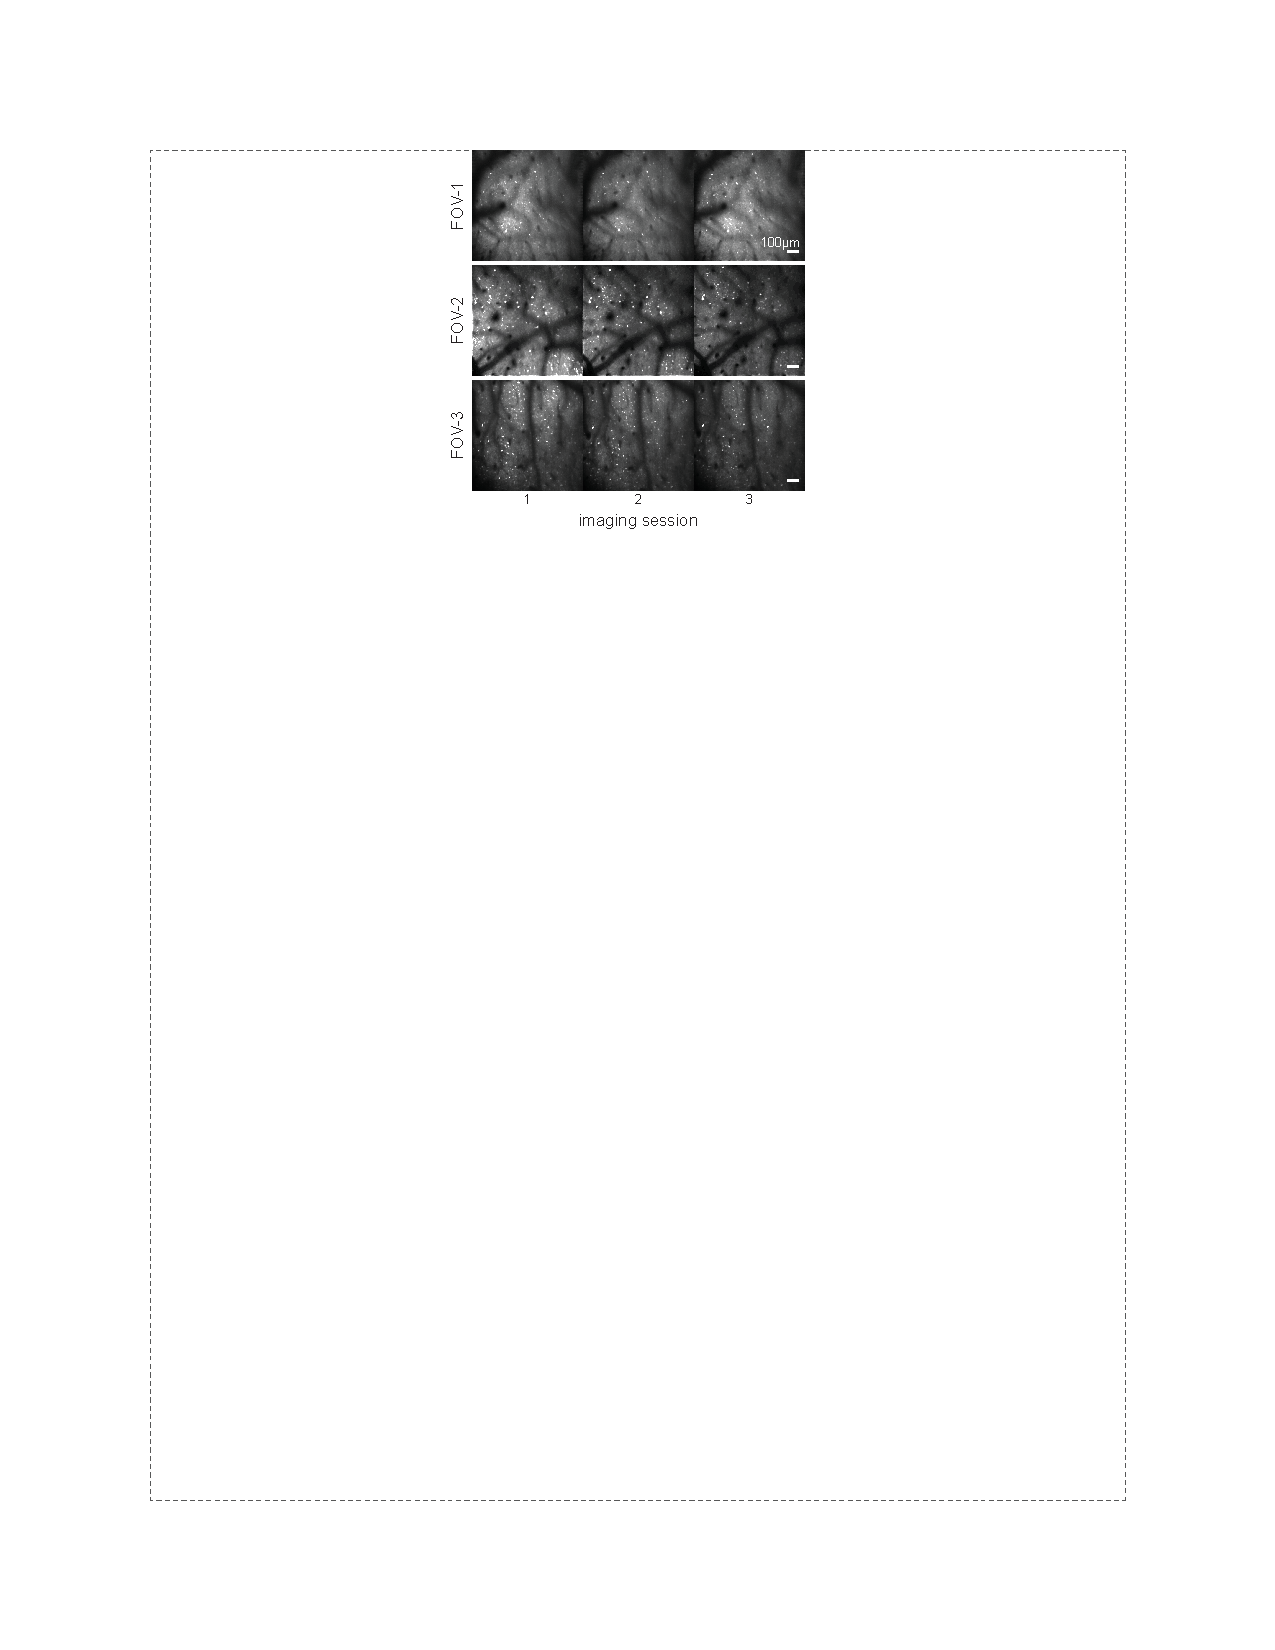
\includegraphics[width=\textwidth]{figures/chapter_2/fig_2-8_multiday_imaging/fig_2-8_multiday_imaging.pdf}
    \vspace{.1in}
    \caption[Multi-day imaging]{Imaging the same cells across days. Each row shows one FOV accessed in three separate days. Each site was identified by eye. Images show the motion-corrected average for each site. No corrections to register one session with the next.    
    \label{fig:multiday_imaging}}
\end{figure}

The kinematic mount for our titanium headplate was not only designed to hold the animal stable, but importantly, to allow precise re-positioning of animals from day to day. In combination with blood vessel landmarks and the unique layout of fluorescent, GCaMP-expressing cell bodies in a given field-of-view in 3-dimensional space, this precise re-fixation allowed us to rapidly relocate the same cells across sessions (Figure\ref{fig:multiday_imaging}). It is difficult in any GCaMP-labeled brain to get the same exact population on each day, due to differences in baseline activity and generic neural tissue movement that occurs across hours. However, the majority of well-labeled cells combined with scanning in depth enabled good matching across sessions. 

% Habituation + shaping
To reduce prohibitively large motion artefacts from rats resisting head-fixation, we developed a shaping procedure to habituate rats for multi-hour sessions (the longest sessions were ~5 hours). Briefly, rats were placed in a red, transparent cylinder also used as enrichment in their home cages, and over the course of several days ($\sim$2-4 days) animals were given decreasing doses of sedative (Midazolam, 1mg/kg) and increasingly long habituation sessions (gradually increasing from $\sim$30 minutes to $\sim$3 hours). We found that rats always struggled in the first habituation session without any sedative, which appeared to be critical to accustom the rats to head-fixation in long sessions. That is, most rats quickly learned that it was not possible to physically remove themselves from the implant. We found even in the first two-photon imaging sessions, rats struggled at the very start, well before acquisition began, and remained quiescent throughout most of the session. Although we did not train animals on a task, observable signs indicated that the animals were relatively calm --- they groomed periodically throughout the session, and accepted water and ate treats while they were head-fixed. 

%%%%%%%%%%%%%%%%%%%%%%%
% Concluding remarks
\section{Concluding remarks}
The methodological developments presented in this chapter provide a reliable series of steps for long-term imaging of cranial windows in awake rats. Many of these methods are readily available in mice, and the past decade of systems neuroscience research has seen the surprising emergence of mice as a powerful model system for studying visual circuits. However, the rat has been an important model across all fields of biology for much longer, from sensory behavior\cite{Lashley1930, REFREF} to spatial navigation\cite{OKeefe1971, Aronov2014, Eichenbaum1990}, to physiological disorders and drug testing\cite{REFREF}. 

We overcome several challenges that have prevented the use of a subset of immensely powerful tools in rat models. First, we developed methods for stably holding an animal by its head, while leaving the rest of its body free to either sit relatively naturally or engage with manipulanda relevant for a behavior task. Second, we fine-tuned standard surgical protocols for cranial window implants that would allow long-term viability for cellular resolution imaging in awake rats. Importantly, we demonstrate a method for accessing some of the most lateral and posterior areas of rat cortex. The combination of hard-to-access imaging planes and the rat's capacity for producing large (and damaging) mechanical forces presented significant challenges. Our custom designs for tiling imaging systems overcome these challenges by rotating the optical axis around the animal, allowing a relatively natural sitting position, which is important both for keeping the animal calm during imaging as well as comfortable enough to willingly engage in behaviors. 

Finally, we engineered a two-photon microscope design that allows a full repertoire of imaging modes, including multi-channel acquisition and large fields of view that can allow multiple areas to be imaged simultaneously in the rat. Lateral areas of the rat are challenging to access with optical approaches as they are difficult to reach with bulky microscopes without putting the animal in an uncomfortable and unnatural position. By developing a method that combines a tilting microscope with head-fixing awake rats, this work overcomes many of the challenges that have made it difficult to study the neural processes underlying known visual behaviors in the rat. Thus, these developments unlock significant avenues of research in rats, particularly in questions involving complex behavior and the various functions of different cortical areas, and the nature of their dynamics during learning or particular behaviorally-relevant contexts. 

%%%%%%%%%%%%%%%%%%%%%%%
% While previous studies have shown used coarse retinotopy to identify the areas in which they were recording, the fine-scale retinotopic organization of cell bodies in any extrastriate area remains unknown. To characterize retinotopic preferences at single-cell resolution, we used the same phase-encoding Fourier paradigm used in wide-field mapping with two-photon calcium imaging.


% % Retino scatter
% Cell bodies exhibited a coarse-scale retinotopic organization. However, retinotopic preferences of neighboring cells were disordered and deviated from the surrounding neuropil in V1, LM and LI {\fig:Figure1f, REFREF, Supplemental 2.2, 2.3, stats REFREF}, consistent with findings in mouse visual cortex \cite{Liang2018, Andermann2011, Marques2018}. Single sweeps of the stimulus evoked robust responses in individual cells. 


% We found an asymmetric expansion of spatial representation along the elevation axis in all areas tested (Figure\ref{fig:2p_retino}). There was a ~2-fold increase in cortical magnification along the visual axis of elevation versus azimuth (REFREF paired t-test, V1: p=#, LmL p=#, Li: p=#). 
% \begin{savequote}[75mm]
% Nulla facilisi. In vel sem. Morbi id urna in diam dignissim feugiat. Proin molestie tortor eu velit. Aliquam erat volutpat. Nullam ultrices, diam tempus vulputate egestas, eros pede varius leo.
% \qauthor{Quoteauthor Lastname}
% \end{savequote}

\chapter{Basic characterizations}
% fig:2p_retino
% fig:rf_examples
% fig:retino_scatter
% fig:rf_aggregate
% fig:vf_coverage

% fig:gratings_examples
% fig:gratings_aggregate
% fig:theta_vs_rf_angle

% Supps:
% rf5_v_rf10
% spherical_correction
% gratings_fitting
% vf_targeting

\newthought{Rats rely on vision} for a many natural behaviors, such as a hunting\cite{REFREF}, jumping and depth perception\cite{REFREF}, and spatial navigation\cite{REFREF}. Over the past few years, a subset of contiguous areas spanning the lateral edge of rat cortex have garnered significant attention due to possible similarities with the primate ventral visual stream. Several studies \cite{Vermaercke2014, Tafazoli2017, Vinken2016NeuralCortex} have investigated these visual areas --- V1, LM, LI, and LL --- specifically in the context of visual object representations in order to test the extent to which single neuron characteristics of primate IT, the highest level of the primate ventral stream, might also be found in the lateral most areas in the rat. 

% Name some known examples for how mice and primates are different.
However, monkeys and rodents, differ in dramatic ways --- on one hand, similarities in how their visual systems solve a given problem are incredibly exciting, as they point to general principles conserved across species. On the other hand, each solution is likely to be influenced by differences in the natural visual statistics by which their visual systems have been shaped. For example, in primates and cats, cells with similar orientation preferences are organized in columnar structures in V1\cite{Blasdel1986}. In contrast, as shown by one of the first two-photon imaging studies of rat V1, and many mouse studies thereafter, rodents have a salt-and-pepper-like organization of orientation preference that does not appear to have an obvious global structure\cite{Ohki2005}). 

Over the past decade, mice have become increasingly popular for studying visual circuits. This is arguably due to the immensely powerful genetic tools combined with chronic, large-scale population recordings, much of which are prohibitively challenging to use in monkeys. In contrast, although rats have long been studied for visually-guided behaviors, large-scale cellular resolution access to their visual cortex has proved to be far more challenging. Our broad-level goal is to bridge the gap between neural circuit access and rich behavioral capacities in the rat. Rats lack a basic characterization of any visual area beyond V1. Such a systematic study provides valuable points of comparison not just with primates, but with other animal models, including mice. 

% ---------------------------------------------------------------
% Experiment design
% ---------------------------------------------------------------
% Broad overview of experiment design -- all the stimuli.
Two overarching goals shaped our experimental design (Figure\ref{fig:experiment_design}). First, we hoped to contribute an immensely powerful method to the existing body of literature on visual object recognition in rats. Several studies have characterized single-unit response properties of lateral extrastriate areas in rats that may be similar to those found in the primate ventral stream\cite{Tafazoli2017, Vermaercke2014, VinkenX, Vermaerke2015}. As such, we know relatively more about single-unit response properties in these lateral areas than in any other extrastriate area of the rat. However, most previous rat studies specifically characterized single-unit responses to object stimuli --- much less is known about more basic response properties of these visual areas. As a parallel goal, we sought to provide a first comprehensive survey of basic, visual response properties across these different cortical areas in the rat using optical imaging. 

% Figure:  Experimental design.
\begin{figure}
    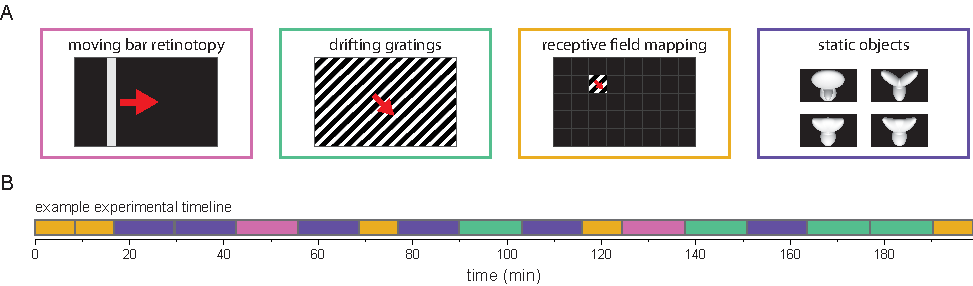
\includegraphics[width=\textwidth]{figures/chapter_3/fig_3-0_experiment_design/fig_3-0_experiment_design.pdf}
    \vspace{.1in}
    \caption[Experiment design]{Experiment design for characterizing visual responses in rat lateral cortex. \textbf{A.} REFREF 
    \label{fig:experiment_design}}
\end{figure}

We focused on the first three of four visual areas targeted by previous electrophysiology studies of object recognition properties of rat visual cortex. These areas, V1, LM, and LI, were the most reliably detected with our combined method of viral expression and wide-field mapping, as described in Chapter 2 (given the somewhat inconsistent nature of viral GCaMP expression in terms of even coverage, area LL was not easy to identify with confidence. See the Discussion below). Using a large battery of visual stimuli (Figure\ref{fig:experiment_Design}), we characterized basic visual response properties of these three areas for the first time with cellular resolution imaging. In the same sessions, we also tested a subset of the complex visual object stimuli used to test the perceptual behavior of rats (behavior described in Chapter 1, neural characterizations described in Chapter 4). Given their potential as areas important for visual object recognition behavior, areas V1, LM, and LI  represent an exciting starting point for combining the powerful tools common in traditional genetic models like mice with the kinds of complex behaviors associated with primates.  

\section{Identification of two-photon imaging sites}
The mirror reflections of the retinotopic gradient in our wide-field maps identified macro-level areal borders. We used these maps to determine which visual areas to target for two-photon imaging sessions. In order to register the two-photon maps to the wide-field maps, we acquired an anatomical volume at the start of each session. This was a surface-level z-stack that captured fiduciary markers in both channels: while the green channel was always used for functional runs (GCaMP), we used the red channel to acquire images of blood vessels filled with a temporary fluorescent dye that was injected at the start of each session (see Methods). Acquiring an anatomical volume also helped for identifying and returning to the same FOV across days. 

Each rat underwent a localizer run prior to any functional sessions. Localizer runs were conducted on a day prior to full functional sessions. These sessions identified which parts of the visual field corresponded to a given imaging site, targeted based on the surface-level vasculature and wide-field areal mapping (see Chapter 2, Figure\ref{fig:retino_mapping}). Two-photon vasculature images were matched offline to the high-resolution images we took of the brain surface in each wide-field mapping session. Once a candidate FOV was found to contain visually responsive cells, and the visual area assignment was validated, it was acceptable for full functional runs, which were the full battery of stimuli used to characterize the FOV (Figure\ref{fig:experiment_design}). Localizer runs were always run again during functional sessions.

We used two types of mapping protocols that targeted different scales of retinotopic organization. The first captured broad retinotopic preferences across the field-of-view using the same cycling bar stimulus used to identify area borders in wide-field maps (see Chapter 2, \ref{fig:retino_mapping}). The second provided a more fine-scaled characterization of individual receptive fields for each neuron in the selected FOV:  we used a time-consuming, albeit highly reliable, approach in which small portions of the visual field were systematically stimulated in a tiled manner to estimate the receptive field positions and extents of all cells. In addition, since only a subset of the experiments used full-field stimuli, it was important to accurately identify the region of visual space to which most cells in a given FOV were responsive and target the stimulus presentation there. 

Once a given FOV was identified as visually responsive, and the receptive field locations of the whole population could be identified, functional runs were conducted on subsequent days. We selected a battery of stimuli to provide a foundation for basic visual response properties in the lateral extrastriate areas of the rat. The final stimulus sets included drifting gratings of multiple orientations, spatial frequencies, and speeds, and a subset of the complex object stimuli used to test rats' perceptual behavior (as described in Chapter 1).

% ---------------------------------------------------------------
% 2p retinotopy
% ---------------------------------------------------------------
% fig:2p_retino (2p setup, coregistration, gradient, cortical mag)
% fig:rf_examples (fine-scaled RF measurements)
% fig:retino_scatter 
% fig:rf_aggregate
% fig:vf_coverage
% ---------------------------------------------------------------

\section{Fine-scale retinotopic organization in rat lateral cortex}
While previous studies have relied on coarse retinotopy to identify the areas in which they were recording, the fine-scale retinotopic organization of cell bodies in any extrastriate area remains unknown. Using the same phase-encoding Fourier paradigm we used to measure retinotopic gradients in wide-field maps, we characterized retinotopic preferences across a given two-photon field-of-view (Figure\ref{fig:2p_retino}A). This method also allowed us to quickly identify and validate that the retinotopic gradient direction measured at the macro scale was aligned with the gradient measured in the two-photon FOV. Two-photon FOVs were registered to wide-field vasculature maps offline by selecting matching points between the two views based on uniquely identifiable blood vessels present in both images. We then used these points to identify a transformation matrix to map one view onto the other (Figure\ref{fig:2p_retino}B, and see Methods). Sweeps of the cycling bar produced robust responses in individual cells throughout the FOV (Figure\ref{fig:2p_retino}D). We observed retinotopic gradients across visual axes of elevation (ventral-dorsal) and azimuth (nasal-temporal) for FOVs imaged in V1, LM and LI (Figure\ref{fig:2p_retino}E). 

% fig:2p_retino 
\begin{figure}
    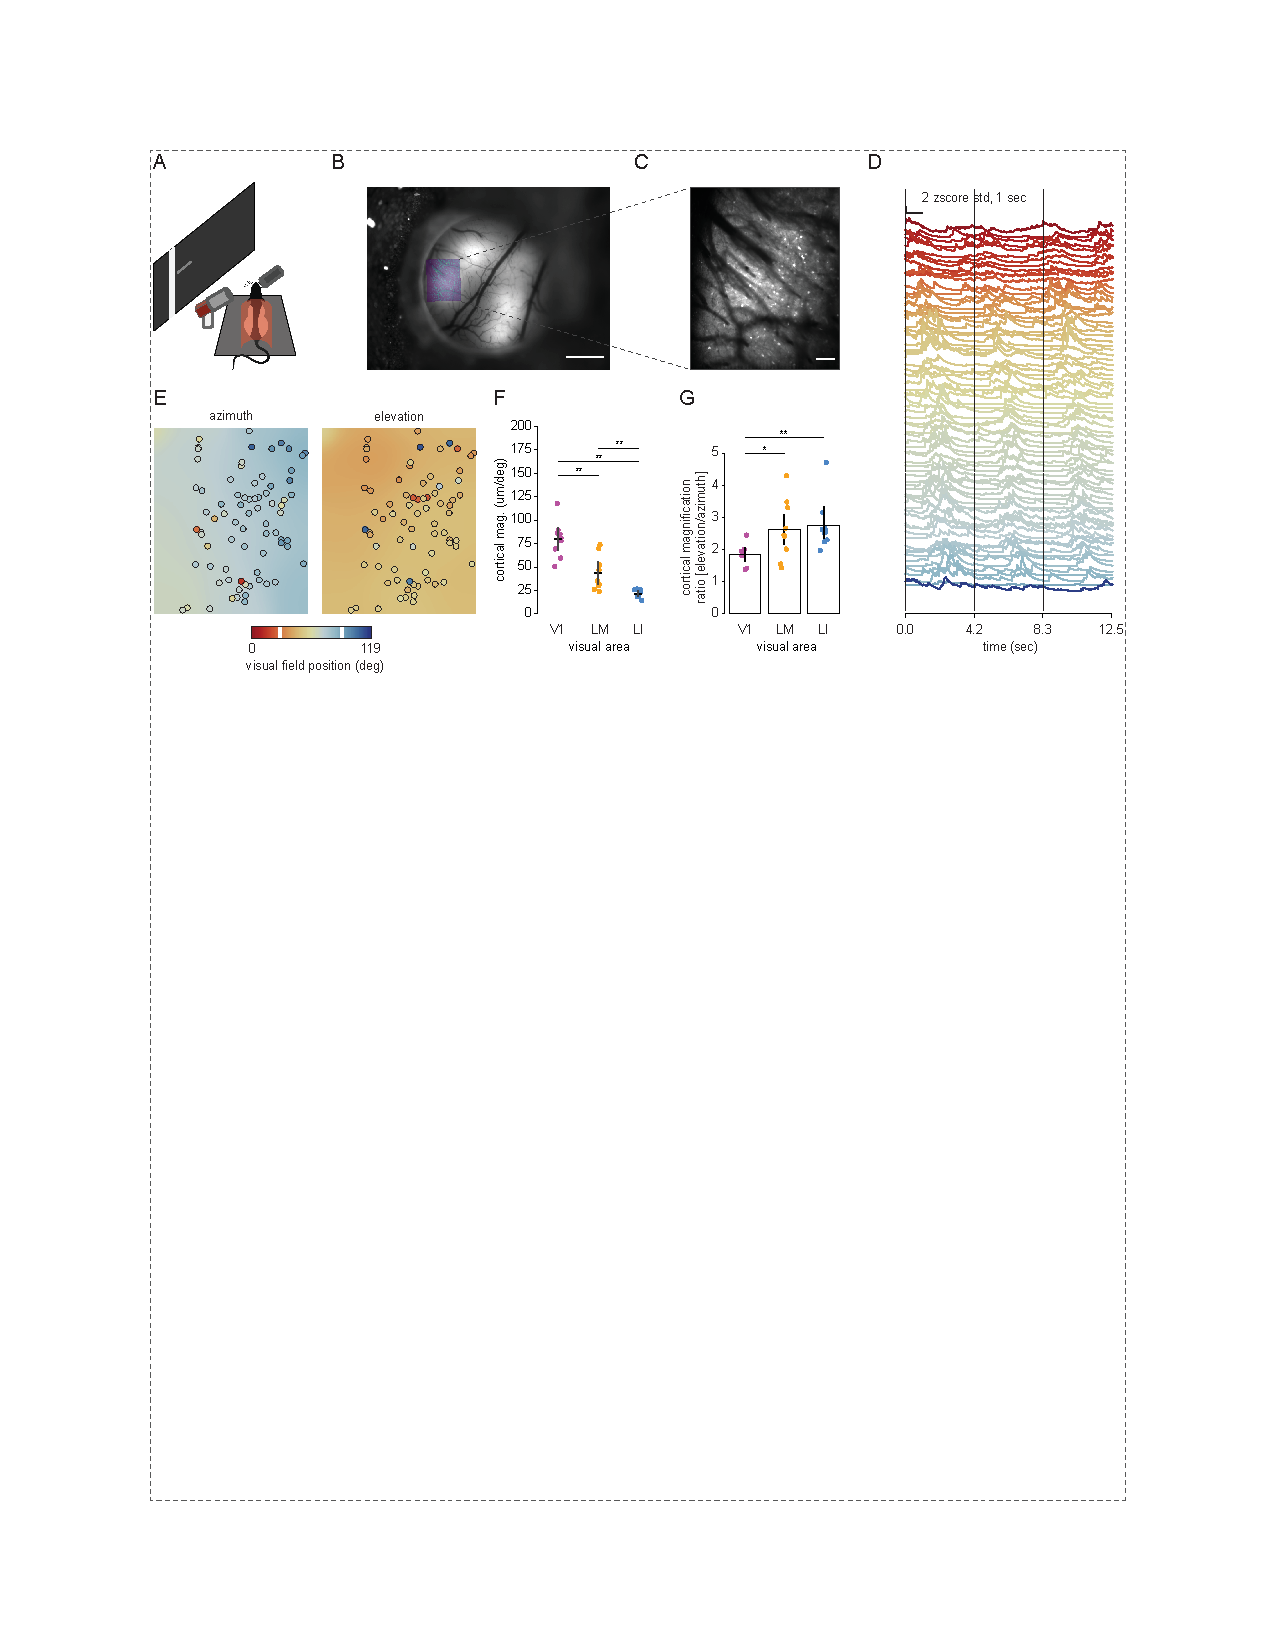
\includegraphics[width=\textwidth]{figures/chapter_3/fig_3-1_2p_retino/fig_3-1_2p_retino.pdf}
    \vspace{.1in}
    \caption[Identification of areas with two-photon imaging]{Coregistration and area identification for two-photon imaging. \textbf{A.} Schematic of imaging experiments in awake, head-fixed rats. 
    \textbf{B.} \textit{Left}: Wide-field image of the surface vasculature in the cranial window of an example rat. The overlay (blue) shows the co-registered anatomical image of the surface vasculature acquired by two-photon imaging. Scale bar, 1mm. 
    \textbf{C.} Example two-photon imaging field-of-view using the standard, large-FOV mode. The FOV is scaled for visualization purposes based its measured pixel size. Scale bar, $100um$. 
    \textbf{D.} Example z-scored timecourses for three cycles of the moving bar stimulus for all identified cells in an imaging site. Condition shown was a white bar (5 degrees of visual angle) moving in the nasal-to-temporal direction across the screen at 0.24Hz. Traces are colored and sorted by each cell's phase at the stimulation frequency (colormap as in \textbf{E}). Dotted lines denote the start of each cycle. 
    \textbf{E.} Pseudo-colored image of retinotopic azimuth (left) and elevation (right) preference obtained by two-photon imaging with the cycling bar stimulus, \textif{i.e.}, the same phase-encoded mapping paradigm used for wide-field mapping. Colors within cell body masks indicate preferred retinotopic locations. Background pixels contain a smoothed estimate of neuropil retinotopic preferences. 
    \textbf{F.} Cortical magnification for each imaging site recorded in areas V1, LM and LI (*: p<0.05, **: p<0.01, Mann-Whitney U-test, REFREF corrected for multiple comparisons). 
    \textbf{G.} Ratio of cortical magnification along elevation to azimuth for each imaging site. Conventions as in \testbf{F}.   
    \label{fig:2p_retino}}
\end{figure}

% ---------------------------------------------------------------
% Cortical magnification
% ---------------------------------------------------------------
\subsection{Cortical magnification is asymmetric}
The particular region and extent of visual space that a patch of cortex represents has important implications for its function. For example, in primates, most areas of the ventral stream over-represent the central visual field, enhancing the processing of features near the fovea\cite{REFREF, Gattass2005CorticalDynamics}. Although mice and rats do not have foveal vision, several groups have shown biases of visual field coverage across visual cortex in mice\cite{Garrett2014, Marshel2011, REFREF}. To quantify how much surface area is devoted to a given unit of visual space in rat extrastriate cortex, we measured cortical magnification in areas V1, LM and LI. Overall, we found that cortical magnification decreased from V1 to LM to LI, consistent with the expectation that larger areas have more cortical real estate for representing a given part of visual space (Figure\ref{fig:2p_retino}F). 

Cortical magnification is not necessarily isotropic, that is, equal along vertical (azimuth) and horizontal (elevation) axes of the visual field. We found an asymmetric expansion along the vertical dimension of visual space in rat V1, as well as in areas LM and LI (Figure\ref{fig:2p_retino}G). This asymmetry is consistent with findings in mouse V1, in which several studies have reported an expanded representation along the vertical dimension of visual space\cite{Garrett2014, Liang2018, Bonin2011}.  

% ---------------------------------------------------------------
% RFs for better measurements (rfs5 vs rfs10)
% ---------------------------------------------------------------
\subsection{Retintopy is disorganized at fine scales}
Interestingly, we observed slight deviations when comparing our smoothed gradient maps to estimated retinotopic preferences of cell bodies (see Figure\ref{fig:2p_retino}E). Previous studies in mouse visual areas indicate the presence of a fine-scale retinotopic scatter from retinal ganglion cell (RGC) inputs, through the lateral geniculate nucleus (LGN), and into V1 and LM\cite{Liang2018, Andermann2011, Marques2018}. However, it remains unknown whether this scatter is present in other extrastriate areas of rodent cortex, and whether this is functionally advantageous in any way or only a byproduct of biological noise. In order to more finely characterize retinotopic preferences of individual cells, we quantified receptive field (RF) properties by stimulating tiled locations across the visual field (Figure\ref{fig:rf_examples}). 

% fig:rf_examples
\begin{figure}[t!]
    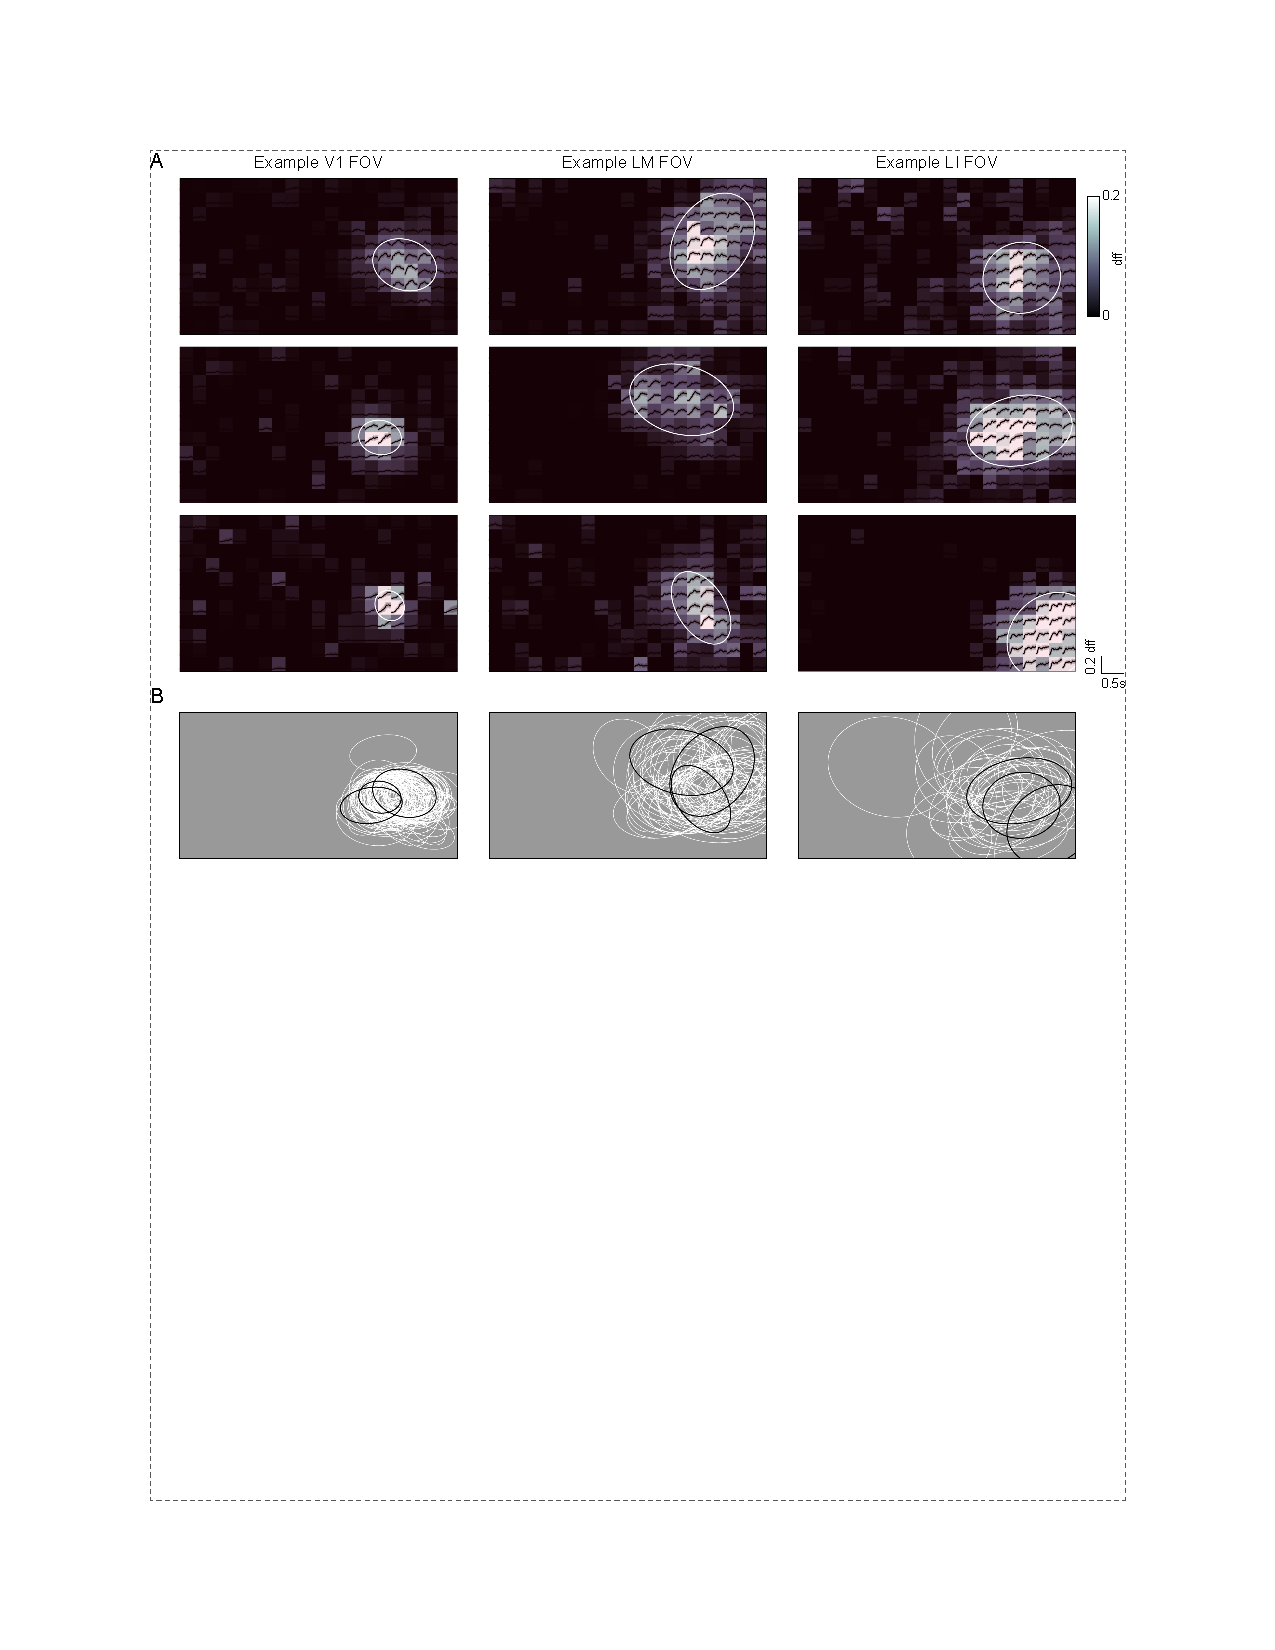
\includegraphics[width=\textwidth]{figures/chapter_3/fig_3-2_rf_examples/fig_3-2_rf_examples.pdf}
    \vspace{.1in}
    \caption[Receptive field mapping]{Mapping receptive fields of single neurons. \textbf{A.} REFREF.
    \label{fig:rf_examples}}
\end{figure}

We used tile sizes of 5 or 10 degrees of visual angle to account for the possibility that cells with larger receptive fields may not be effectively stimulated by small stimuli, and vice versa, that cells with small receptive fields or sensitivity to surround suppression may be under-stimulated by large stimuli. Consistent with previous studies that mapped receptive fields in mice\cite{DeVries2019}), the larger, 10 degree tile size produced more and stronger responses for cells in extrastriate area LI, while the 5 degree tile size worked well for areas V1 and LM. To confirm that the stimulus size did not dramatically affect any of our receptive field measurements, we directly compared the receptive fields of cells in which we obtained fits using both the small and large stimulus sizes (REFREF Figure\ref{fig:suppfig}). Overall, we found that V1 cells had slightly underestimated receptive field sizes when using the larger stimulus size. Importantly, for the goal of obtaining precise retinotopic position estimates for each cell, defined as the center of the fit receptive field, receptive field position meaured with small and large stimuli were tightly correlated, for both azimuth and elevation positions (Supplemental Figure\ref{suppfig:rf5_rf10} REFREF). We did not observe systematic biases in any of the other receptive field metrics, and thus selected whichever of the two stimulus sizes produced the most well-fit receptive fields on average for LM (smaller, 5-degree tile size) and LI (larger, 10-degree tile size). 

% ---------------------------------------------------------------
% \subsection{Retinotopic scatter is asymmetric}
% Average cortical scatter
% ---------------------------------------------------------------
To quantify scatter, we compared measured receptive field positions to predicted positions. Specifically, for a given population of cells recorded at an imaging site, we calculated the global retinotopic gradient using smoothed estimates of neuropil preferences across the FOV (Figure\ref{fig:retino_scatter}A). Since the vertical and horizontal axes of the visual field representation is not necessarily aligned to anterior-posterior or medial-lateral axes of the cortical surface, we computed a simple transformation that identified the directions of maximal change along each direction based on the smoothed neuropil retinotopic map. Specifically, to compute the spatial axis corresponding to the global retinotopic gradient for each axis, we used the average gradient vector across the FOV. The smoothed retinotopic map was then 
projected along this mean gradient vector, and the predicted location of each pixel was defined as its projected location along this new spatial axis (see Methods).  

After making this correction, we found that most cell bodies exhibited a coarse-scale retinotopic organization (Figure\ref{fig:retino_scatter}B), Pearson's correlation coefficient, V1: r=REFREF, p<0.01; LM: r=REFREF, p<0.01; LI: r=REFREF, p<0.01). However, at the level of neighboring cells, retinotopic preferences were disordered and deviated from the expected preferences based on relative cortical location. To ensure the observed scatter was not simply measurement noise, we identified true deviants by estimated 95\% confidence intervals for all measured receptive field positions. Specifically, for each cell, we determined whether the 95\% confidence interval estimated for its receptive field position along the vertical or horizontal axes overlapped with the 95\% confidence interval estimated for the linear fit defining its predicted receptive field locations based on cortical position.  

\begin{figure}[t!]
    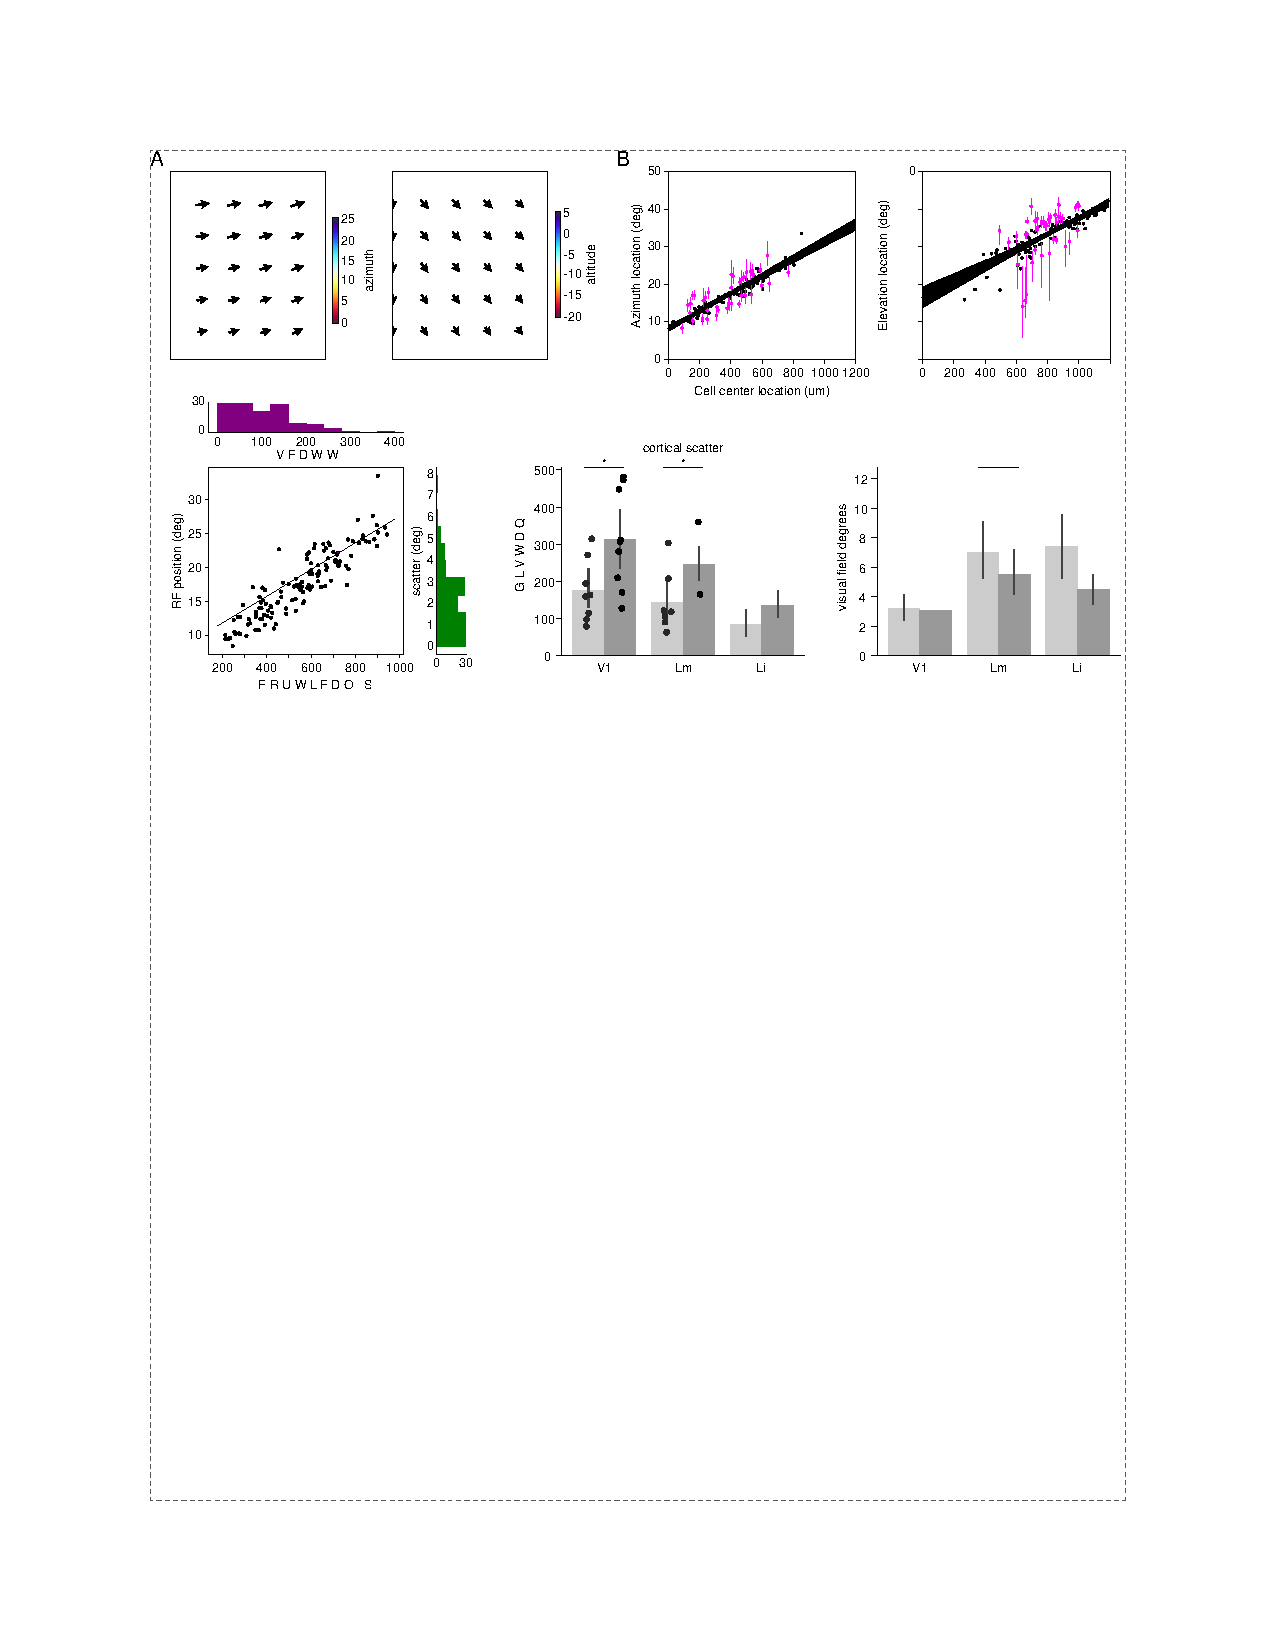
\includegraphics[width=\textwidth]{figures/chapter_3/fig_3-3_retino_scatter/fig_3-3_retino_scatter.pdf}
    \vspace{.1in}
    \caption[Fine-scale retinotopic scatter]{Fine-scale retinotopic scatter in lateral extrastriate cortex. 
    \textbf{A.} Smoothed estimates of neuropil retinotopic preferences for an example V1 FOV for azimuth (left) and elevation (right). Colormap shows visual field position in degrees of visual angle.
    \textbf{B.} Each cell's retinotopic preference versus cortical location along azimuth (left) and elevation (right) axes of retinotopic progression for the example field of view shown in \testbf{A}. Black line: linear fit to retinotopic gradient. Shaded bands, 95\% CI. Black dots: individual cells in the field of view for which reliable receptive field estimates were made (see Methods). Magenta dots: True deviants that significantly deviated from predictions. Magenta lines, 95\% CI. 
    \testbf{C.} Illustration of scatter in cortical position (purple) and scatter in visual field position (green) based on predicted retinotopic preferences based on cortical position. Line, linear fit of the predicted retinotopic gradient, based on the projection of the neuropil map onto the mean gradient vector (as shown in \textbf{A}). Dots, measured receptive field position and cortical position for each cell in an example FOV. Green vertical line indicates deviation in preference from the mean retinotopic gradient ("visual field scatter" in degrees of visual angle scatter). Purple horizontal line indicates the distance of a cell from its expected cortical location in the absence of scatter ("cortical distance scatter" in $um$). 
    \textbf{D.} Average amount of scatter in cortical distance (left) and visual field position (right) for each imaging site recordedin areas V1, LM, and LI. Each dot represents scatter along azimuth (light gray) or elevation (dark gray) for a given FOV.
    \label{fig:retino_scatter}}
\end{figure}

% Overall scatter & asymmetric scatter in X, Y
To quantify the scale of scatter, that is, the extent to which scatter in the receptive field position corresponds to or is offset by scatter in a cell's cortical position, we measured deviations along cortical distance and visual field position for each cell (Figure\ref{fig:retino_scatter}C). Overall, average scatter in cortical space decreased from V1 to LM to LI (Figure\ref{fig:retino_scatter}D, V1: $\sim$239.09+/-REFREF$um$, Lm: $\sim$163.48+/-REFREF$um$, Li: $\sim$127.17+/-REFREF$um$), corresponding to average retinotopic displacements that increased from V1 to LM to LI (V1: $\sim$2.9; LM: $\sim$5.3; LI: $\sim$6.5 degrees of visual angle). This relative pattern is consistent with the relatively smaller cortical size of areas LM and LI relative to V1 (that is, larger area, more room for error).  

Notably, the observed retinotopic scatter was asymmetric between vertical and horizontal dimensions:  deviations from predicted cortical locations were ~2 fold larger along elevation than azimuth (V1: REFREF in azimuth, REFREF in elevation; Lm: REFREF in azimuth, REFREF in elevation; Li: REFREF in azimuth, REFREF in elevation). In V1, this asymmetric scatter in cortical position was roughly proportional to cortical magnification --- that is, for a given unit of visual field space, we observed $\sim$2-fold expansion in cortical space  for elevation, relative to azimuth, and we see a proportional amount of scatter. In LM and LI, however, we observed less scatter in predicted receptive field positions along the elevation axis than would be expected from the measured cortical scatter if scatter was proportional to the cortical magnification of elevation over azimuth.


% ---------------------------------------------------------------
% RF properties
% ---------------------------------------------------------------
% RFs are anisotropic, elongated along azimuth
% -better resolution in elevation? -- horizontally oblong
Given the observed asymmetry in cortical magnification along azimuth and elevation (see Figure\ref{fig:retino_scatter}), we asked whether this asymmetry was also present at the level of individual receptive field shapes. A hallmark of hierarchically-organized visual areas, based on the primate ventral stream, is a gradual increase in average receptive field size\cite{RustREFREF, Vermaerke2014, Siegle2019AAreas, Tafazoli2017}. We quantified overall receptive field size as the average widths along the horizontal and vertical axes (Figure\ref{fig:rf_aggregate}A). Consistent with previous electrophysiology measures in rats\cite{Vermaercke2014, Tafazoli2017}, we found that average receptive field size increased from V1 to LM to LI (V1: median 8.8+/-REFREF, LM: 10.5+/-REFREF degrees, LI: 13.1+/-REFREF degrees of visual angle, p<0.01, Mann-Whitney U-test, p<0.01, fdr-bh corrected for multiple comparisons REFREF). This was true regardless of whether comparisons were restricted only to cells fit using either the small or large stimulus size for all visual areas (Figure\ref{fig:Supp} REFREF).  

% Interestingly, the amount of scatter in the predicted receptive field locations corresponded to roughly half or less than the average receptive field size of each visual area (REFREF, V1: ~$9.49+/-REFREF$, Lm: ~$10.61+/-REFREF$, LI: ~$13.25+/-REFREF$ degrees of visual angle). However, at the level of individual cells, we observed no correlation between receptive field size and retinotopic scatter (Supp Figure REFREF), stats, Pearson’s correlation, V1: REFREF, p=REFREF, Lm: REFREF, p=REFREF, Li: REFREF, p=REFREF).

\begin{figure}[t!]
    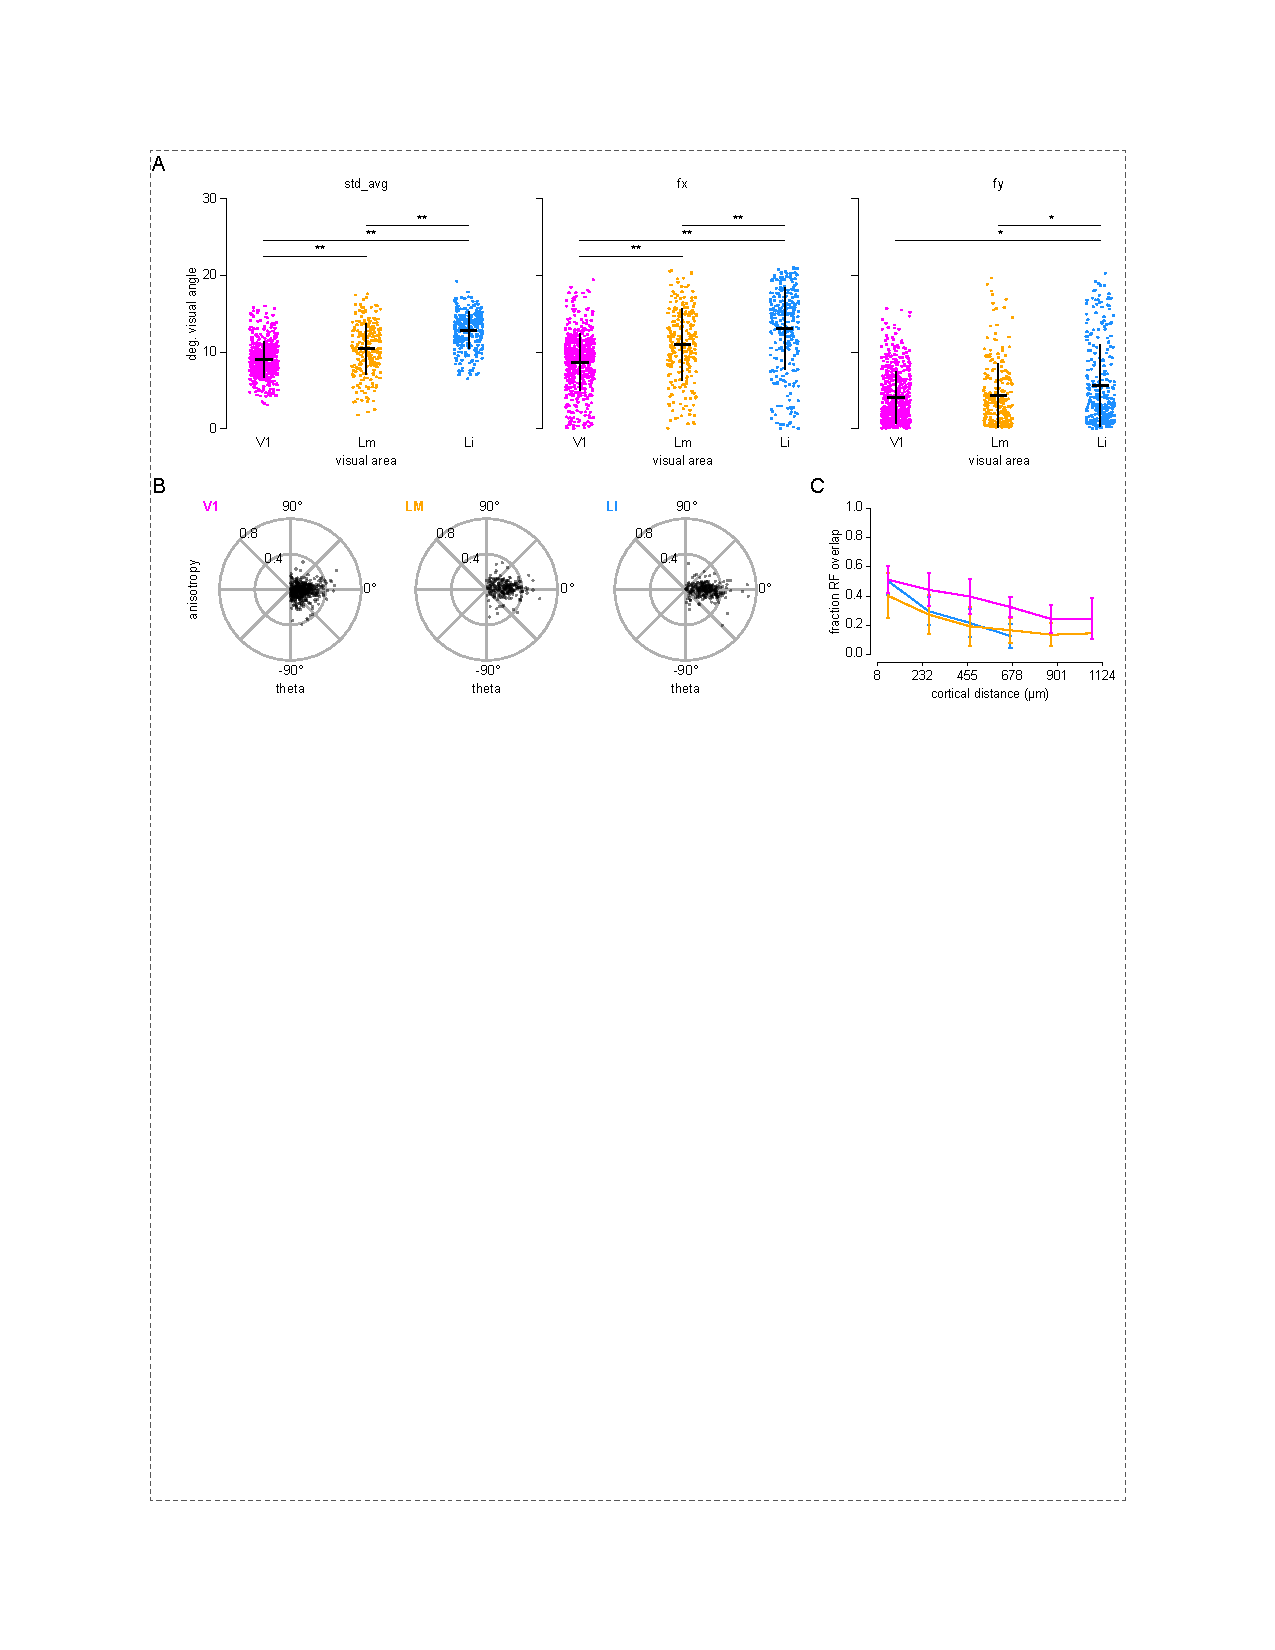
\includegraphics[width=\textwidth]{figures/chapter_3/fig_3-4_rf_aggregate/fig_3-4_rf_aggregate.pdf}
    \vspace{.1in}
    \caption[Receptive field properties]{Receptive field properties across lateral extrastriate cortex. 
    \textbf{A.} \textit{Left}: Average size, measured as half-width at half-max (HWHM) of a double Guassian fit. Also shown is the projection of the major axis of each ellipse onto the horizontal (\textit{middle}) or vertical (\textif{right}) axes of visual space for each cell. Each dot represents one cell. Horizontal and vertical bars, mean and SD across cells. 
    \textbf{B.} Anisotropy, measured as the ratio of major to minor axes of the fit ellipse, as a function of receptive field angle. Each dot is a cell. Anistropy ranges from 0 to 1, where 0 represents perfectly isotropic receptive fields (a circle), and 1 represents an extremely linear receptive field. Receptive field angles of 0 represent orientations parallel to the horizontal axis, and 90 degrees represents orientation parallel to the vertical axis.
    \textbf{C.} Receptive field overlap as a function of cortical distance. For each pair of cells, overlap is measured as the intersection of their receptive fields divided by their union. Error bars, SD.  
    \label{fig:rf_examples}}
\end{figure}

Interestingly, when we split receptive field size according to the extent of vertical or horizontal space covered, we found that the horizontal dimension was consistently larger, suggesting that most receptive fields were anisotropic (Figure\ref{fig:rf_aggregate}A). For each cell, we calculated the degree of anisotropy by taking the ratio of the major and minor axes of the fit ellipses. Most receptive fields exhibited some degree of anisotropy, with receptive field angles biased toward 0 degrees, elongated along their azimuthal dimension (Figure\ref{fig:rf_aggregate}B). 
% However, we did not observe strong relationships between anisotropy and retinotopic scatter (REFREF, Supplemental 3.3) nor between angular bias in anisotropy (horizontally or vertically anisotropic, see Methods) and retinotopic position (REFREF, Supplemental 3.4). 
% -Sit & Goard, bias for cells representing LOWER visual field, stronger coherent motion response -- spatial asymmetry in motion representation/sensitivity

% Spherical correction check:
% ---------------------------------------------------------------
To confirm that the observed receptive field anisotropy was not simply due to variable screen distance, we calculated the same metrics with a spherical correction. Typically, in visual field mapping studies, the screen is close enough to the animal's eye that significant warping can occur at the edges of the visual field, relative to the portions directly in front of the animal, producing a "fishbowl" effect. Experimenters often correct for this distortion by presenting an inversely distorted stimulus, effectively reversing the warped appearance (see Figure\ref{fig:spherical_correction} REFREF). Alternatively, the stimuli can be presented as is, on the flat monitor, and the measured responses can be transformed according to the predicted perceived distortion. Using this latter transformation, we found little to no qualitative difference in the relative receptive field metrics: receptive field sizes increased from V1 to LM to LI, receptive fields were anisotropic in all three areas, and this anisotropy was largely biased toward elongations along the horizontal axis (SUPPFIGURE REFREF).

% Maybe this is for better visual field coverage?
These receptive field asymmetries are consistent with the observed expansion in the cortical representation of visual space along the vertical axis in that the relative compression of the vertical axis in receptive field shape might enable higher-resolution representations along the vertical dimension than if receptive fields were perfectly isotropic. To quantify whether or not this property might afford more precise visual field representations, we compared how faithfully the receptive field organization of a population followed what would be predicted by highly-organized, retinotopic structure. 

% Vf coverage W/ and W/OUT scatter?
\begin{figure}[t!]
    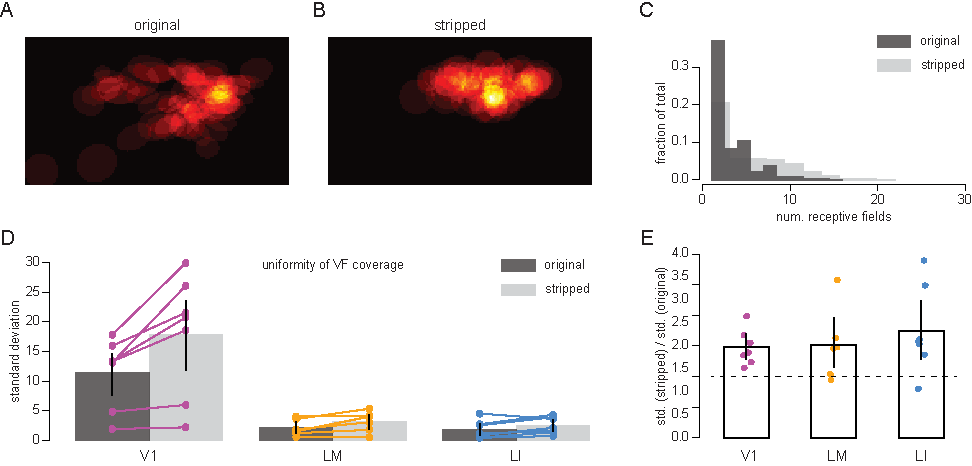
\includegraphics[width=\textwidth]{figures/chapter_3/fig_3-5_vf_coverage/fig_3-5_vf_coverage.pdf}
    \vspace{.1in}
    \caption[Compensatory visual field coverage]{Gains in visual field coverage due to scatter. 
    \textbf{A.} REFREF.
    \label{fig:vf_coverage}}
\end{figure}

Specifically, we wondered whether these irregularities might allow, for example, enhanced visual field coverage. For all simultaneously recorded cells in a given imaging site, we compared how the distribution of receptive fields across the visual field changed if all irregularities were corrected. To nullify retinotopic scatter, we assigned the predicted retinotopic position to each cell, and to nullify receptive field irregularities, we assigned size along each axis to be equal to the average of the two axes such that simulated receptive fields were perfectly isotropic (Figure\ref{fig:vf_coverage}A). We calculated the variance of the distributions of receptive field counts across the visual field as a measure of how uniformly the receptive fields covered the visual field:  higher variance indicates receptive fields are clustered in select locations, while lower variance indicates receptive fields are more evenly spread out (Figure\ref{fig:vf_coverage}B). Overall, simulated receptive field distributions resulted in a less uniform visual field coverage than measured distributions (Figure\ref{fig:vf_coverage}D), paired Wilcoxon signed-rank test: V1, p=0.01; LM, p=0.05; LI, p=0.07). The fold-change in variance was greater than 1 (no difference) for all imaging sites, though we did not observe significant differences between visual areas (Figure\ref{fig:vf_coverage}E). 



% ---------------------------------------------------------------
% Gratings
% ---------------------------------------------------------------
\section{Orientation and direction tuning}
Given the observed retinotopic disorder at small micron scales, we asked whether neurons might be organized by tuning to other visual features. In highly visual animals, like primates and cats, orientation tuning exhibits a spatial organization in which columns of cortex show repeating "pinwheel" structures of preferred orientations\cite{REFREF}. In contrast, studies of rodent visual cortex have shown a disorganized, "salt-and-pepper" organization\cite{Ohki2005, REFREF}, even in more visual rodents like the squirrel\cite{VanHooser2005FunctionalRodent, REFREF}. The lack of clear global structure in one but the presence of clear orientation selectivity in both rodents and primates suggests that they represent alternative paths to achieving the same functionality.

\begin{figure}[t!]
    \includegraphics[width=\textwidth]{figures/chapter_3/fig_3-6_gratings/fig_3-6_gratings.pdf}
    \vspace{.1in}
    \caption[Responses to drifting gratings]{Tuning profiles for drifting gratings.
    \textbf{A.} Drifting gratings that varied in direction, spatial frequency, and speed were presented within localized apertures matched to the average receptive field sizes of a given FOV or as full-field stimuli.
    \textbf{B.} Example V1 FOV with colored circles representing each cell's preferred direction (see Methods).
    \textbf{C.} Example traces for the cells marked in \textbf{B}. 
    \textbf{D.} Normalized histogram of preferred directions for all well-fit cells in V1 (left), LM (middle), and LI (right). 0 represents vertically-oriented stripes drifting toward the animal's nasal direction, and 90 represents a horizontally-oriented grating drifting upward.
    \textbf{E.} Cumulative distributions of axis-selectivity index (left) and direction-selectivity index (right) for cells in V1 (magenta), LM (orange), and LI (blue).
    \textbf{F.} Distributions of relative preferences for high and low spatial frequency (left), apertured and full-field gratings (middle), and slow and fast speeds (right) for cells in V1 (magenta), LM (orange), and LI (blue).
    \textbf{G.} Signal correlations as a function of cortical distance for each pair of simultaneously recorded cells. Error bars, SD across imaging sites.  
    \label{fig:gratings}}
\end{figure}

To expand on known characteristics in rodent V1 to extrastriate areas in the rat, we measured calcium responses to drifting gratings over a range of directions, spatial frequencies, speeds, and sizes (Figure\ref{fig:gratings}A-C). For each cell, we estimated tuning curves using bootstrapped estimations with multiple criteria for evaluating the stability and goodness-of-fit (see Methods)\cite{Liang2018}. These steps ensured that all cells included had clear and consistent tuning based on single- or two-peaked Gaussian functions. Consistent with previous studies in rats and other rodents, we found a rough salt-and-pepper organization in V1 FOVs, as well as LM and LI FOVs (see Figure\ref{fig:gratings}B for an example FOV). Overall, we observed a bias in the relative direction preferences across cells. Specifically, we found that cardinal axes were over-represented in areas V1 and LM, though less so in LI (Figure\ref{fig:gratings}D). In particular, a large fraction of V1 cells preferred horizontally-oriented, vertically-moving gratings.  

To determine the extent to which these biases were specific to axes of motion or particular directions of motion, we calculated an index of axis- and direction-selectivity for each cell. Visually responsive cells were classified as responsive to a given direction of motion (direction-selective, DS), or to opposing directions of motion along a given axis (axis-selective, AS), or neither direction- or axis-selective. Overall, we found that the fraction of cells tuned to axis or direction was similar across areas V1, LM and LI (REFREF+/-REFREF), using conservative measures of selectivity and tuning. The three areas differed in their relative fractions of axis selective and direction selective index levels. While axis selectivity significantly decreased from V1 to LM to LI (REFREF), we found that direction selectivity was significantly greater in LI than V1 or LM (REFREF). 
% REFREF compare with othres? Girman looks similar, but mouse like vertical stuff? check marques et al.

Since axis and orientation selectivity are influenced by spatial frequency and temporal frequency\cite{REFREF}, our aggregate metrics of these preferences relied on each cell's most preferred stimulus configuration, that is, we calculated tuning curves for a cell at the particular combination of size, spatial frequency, and speed that elicited the largest responses and the best fits. To determine whether cells had clear preferences across a given direction preference for any of these metrics, we also compared spatial frequency, size, and speed preferences at each cell's preferred orientation (Figure\ref{fig:gratings}F). Since we only tested two levels, one high and one low, for each of the non-direction metrics, we calculated a preference index for each (see Methods). We did not observe any clear differences between visual areas in their average preference for either the lower or higher spatial frequency tested (0.1 and 0.5 cycles per degree, respectively), nor for the slower or faster speeds (10 versus 20 degrees per second). We did observe a preference for the apertured gratings in V1 cells, consistent with effects of surround suppression.

% Orientating tuning similarity v distance?
To compare overall tuning preferences across the range of tested gratings conditions, we created an averaged tuning profile for each cell, defined as the trial-averaged response to each condition, and measured similarity as the correlation coefficient between tuning profiles (Methods). If visual areas exhibit a purely salt-and-pepper organization, tuning similarity and cortical distance should be independent. To determine the extent to which cells might be organized according to their tuning to drifting gratings, we compared the tuning profiles between cells to their cortical distance, defined as the distance between each cell’s center of mass in the image plane. On average, we found no observable relationship between cortical distance and tuning similarity for areas V1 and LM, though there was a slight reduction at the largest distances for LI cell pairs (Figure\ref{fig:gratigns}G). 

% Signal correlations vs. percent-overlap?.
To determine the extent to which similarity in tuning might be explained by receptive field properties, we also looked at signal correlations as a function of receptive field overlap. Given the observed anisotropies in receptive field shape, we wondered whether a cell's direction or axis preference was related to the orientation or angle of its receptive field. That is, a cell highly tuned to vertical (upward or downward) motion might have a receptive field elongated along the vertical dimension, parallel to the preferred direction of motion. On the other hand, the receptive field might be elongated along the axis perpendicular to direction of motion (horizontally elongated), reflecting the cell's preferred tuning to horizontal edges. We were largely limited by the low numbers of cells in which we measured robust receptive field fits and strong direction tuning fits. However, of the few cells for which both metrics could be confidently measured, we found that receptive field orientations roughly matched axis preferences of neurons in V1 for cells with horizontally-oriented receptive fields and vertically-moving gratings (REFREF SuppFigure). 

% \begin{figure}[t!]
%     \includegraphics[width=\textwidth]{figures/chapter_3/ori_rfs/ori_rfs.pdf}
%     \vspace{.1in}
%     \caption[Receptive field shape and edge tuning]{Feature tuning in lateral cortex. \textbf{A.} REFREF.
%     \label{fig:ori_rfs}}
% \end{figure}

% Discussion.
\section{Concluding remarks}



% \begin{savequote}[75mm]
% Nulla facilisi. In vel sem. Morbi id urna in diam dignissim feugiat. Proin molestie tortor eu velit. Aliquam erat volutpat. Nullam ultrices, diam tempus vulputate egestas, eros pede varius leo.
% \qauthor{Quoteauthor Lastname}
% \end{savequote}

\chapter{Object representations in lateral visual cortex}
\newthought{Shape is a diagnostic feature} of object identity. Visually similar objects, such as a pear and an apple, can be grouped together by certain shared visual features. On the other hand, different images or views of any one object can look dramatically dissimilar, yet still belong to the same object (REFREF example?). In the first chapter, we established the behavioral ability of rats to perform visual object recognition and quantified their perceptual choices of object similarity. We next turned our attention to the neuronal substrates of these abilities. 

% Neural subtrates of object recog. -- what do we know from primates.
In the primate brain, the ventral visual pathway is thought to transform non-diagnostic, low-level representations of features that may be common to many different objects into high-level representations that are both diagnostic of object identity, or selective for a given object, and robust to variations in particular appearance, or tolerant to identity-preserving transformations. 

Primate visual cortex is arranged hierarchically, with visual inputs from the thalamus first arriving in so-called ``striate'' cortex (also known as area V1), before being processed and forwarded through a successive chain of hierarchically-organized visual areas (area V2 > area V4 > inferotemporal cortex) curving along the ventral surface of the brain. Along each stage of the ventral stream, there is a gradual increase in object selectivity and tolerance, culminating in area IT, at the highest level of the ventral pathway. 

Several key trends have been observed in the response properties of visual neurons as one progresses from ``lower'' to ``higher'' visual areas along this ventral pathway. First, the region of visual space that a given cell responds to (the ``receptive field'') gradually increases as one moves along the ventral pathway, with receptive fields in the highest stages of visual cortex sometimes responding to up to half of the visual field\cite{op2000spatial}. Meanwhile, selectivity for complex object features also increases along the ventral visual pathway, with neurons in later stages of the pathway responding only to very particular configurations of features\cite{Desimone1984, Logothetis1996}.  Critically, as one progresses along the ventral pathway, neurons also exhibit greater tolerance to identity-preserving transformation of the retinal image -- that is, neurons tend to retain their selectivity for particular object features even if those features are, for instance, moved around on the retina, or scaled up or down in size\cite{Ito1995}.These combined features of selectivity and tolerance are in many ways the key computational hallmarks of high-level vision\cite{DiCarlo2007, DiCarlo2012}. 

% Previous rodent studies
\section{Lateral visual cortex exhibits some of the same core properties found in primates}
Anatomical studies have shown that the connectivity of rodent visual cortex observes a similar hierarchical pattern, with thalamic inputs arriving in an analogous striate area V1 in posterior of the brain, and then projecting ventrally to a series of interconnected extrastriate areas\cite{Coogan1993, ETC}. However, while these areas have been characterized anatomically, much less is known about their function.

Since 
% shape selectivity
% natural vs scrambled
% vs. category representations (Vinken)
% tolerance

Consistent with previous studies in rats, and what might be expected from a primate-like hierarchical organization, we observed increasing receptive field sizes in areas V1, LM, and LI (see Chapter 3). However, consistent with studies in mice, we also found asymmetries in visual field representations and motion tuning preferences that may be particular to rodent visual cortex. To determine the extent to which rat lateral visual cortex intrinsically exhibits properties thought to be important for spontaneous, as opposed to learned, object recognition behavior, we recorded from neural populations in awake, naive rats presented with a subset of the same stimuli used for the trained rats (see Chapter 1, Figure\ref{fig:behavior_generalization}) to probe axes of transformation in which object identity is either preserved or gradually morphed to a new identity across changes.


% ---------------------------------------------------------------
% Single neuron selectivity and tolerance
% ---------------------------------------------------------------
\section{Single neurons exhibit selectivity and tolerance}
One key feature of the primate ventral stream is a gradual increase in shape or object selectivity and a parallel increase in tolerance to identity-preserving transformations. Previous studies have shown that single-units in monkey IT exhibit a trade-of between these properties: neurons that are highly selective are less tolerant to identity-preserving transformations and highly tolerant neurons are not as selective to particular objects\cite{Zoccolan2007}.

To determine whether single neurons exhibited similar characteristics in rat visual areas, we first measured single neuron response profiles in areas V1, LM, and LI. For identity-changing transformations, we tested a subset of the morphs used to probe trained animals’ naive perceptual boundaries (see Figure\ref{fig:behavior_generalization}\textbf{REFREF}), and for identity-preserving transformations, we tested a subset of sizes covering the range of stimulus sizes used to test behavioral generalization to identity-preserving transformations (see Figure\ref{fig:behavior_generalization}\textbf{REFREF}). Since size changes come with large changes in luminance, we also presented a subset of full-screen gray-scale stimuli that were luminance-matched to each size tested (Figure\ref{fig:selectivity_tolerance}\textbf{A}).

\begin{figure}[t!]
    \includegraphics[width=\textwidth]{figures/chapter_4/fig_4-1_single_cell_selectivity_tolerance/fig_4-1_single_cell_selectivity_tolerance.pdf}
    \vspace{.1in}
    \caption[Selectivity and tolerance in single neurons]{Selectivity and tolerance in single neurons. 
    \textbf{A.} Experiment design:  5 stimulus sizes (green box) were used to test identity-preserving transformations, and nine morph levels (purple box) were used to test identity-changing transformations. 5 size-matched luminance stimuli (fullscreen, grayscale; orange box) were also included to control for luminance differences due to changes in size. 
    \textbf{B.} Schematic of flattened rat visual cortex highlighting the path of lateral visual areas highlighted in the current study. \textbf{C.} Morph selectivity (left) and size tolerance (right) for an example V1 FOV (see Methods). Thin, black curves denote tuning profiles for single cells. Colored lines point out individual cells whose averaged timecourses are shown for each tested condition below. Purple corresponds to the first set of traces (middle), while green corresponds to the second set of traces (bottom). Each timecourse is arranged as shown in \textbf{A}. Black lines and shading show mean and SEM across repetitions of each stimulus condition. 
    \textbf{D.} Same as \textbf{C}, but for an example LM FOV.
    \textbf{E.} Same as \textbf{B} and \textbf{C}, but for an example LI FOV.
    \textbf{F.} Distributions of size tolerance across all cells measured in areas V1, LM, and LI. Each dot is a cell, and black lines denote mean and SD across cells.
    \textbf{G.} Same as \textbf{F}, but for single cell measures of morph selectivity. 
    \textbf{H.} Correlation between size tolerance and morph selectivity for example V1 (left), LM (middle), and LI (right) FOVs. Each dot is a cell. Black line and shading, linear fit and 95\% CI.
    \label{fig:selectivity_tolerance}}
\end{figure}

All areas contained a diverse range of object selective and size tolerant cells. For example, even in one V1 FOV, we found cells that exhibited clear size tuning without morph selectivity, morph tuning that was preserved across different sizes, as well as luminance-tuned cells that were also sensitive or insensitive to the different morphs and sizes (Figure\ref{fig:example_blob_responsesREFREF}). 

Overall, we found that across our object stimuli, cells in LI had the lowest lifetime sparseness, while cells in V1 and LM were similarly high in sparseness (REFREF, stats, Mann-Whitney U Test, multiple comparisons). Since the images varied in morph level and size, the sparseness observedin V1 and LM could reflect a higher selectivity for morph shapes or a lower tolerance for varying sizes. To quantify the amount of object selectivity and tolerance, we calculated a morph selectivity index (MX) and a size tolerance index (ST) for each cell\cite{Zoccolan2007}. We found a range of tuning profiles across cells that was comparable between the three areas (Figure\ref{fig:selectivity_tolerance}B-D). On average, we found that relative to V1 and LM, LI cells were both less selective to morphs and more tolerant to size (Figure\ref{fig:selectivity_tolerance}E-F). Notably, this difference was not attributable to overall lower response magnitudes in LI: although we found fewer LI cells selective or responsive to the object stimuli overall, of the cells that were responsive, response magnitudes were comparable across areas (REFREF). 

It is possible that the relatively higher average morph selectivity in V1 and LM cells reflects greater sensitivity to overall luminance values. To characterize the extent to which size or morph tuning simply tracks luminance sensitivity, we calculate the correlation between each cell's size tuning curve and its tuning curve for the size-matched luminance stimuli (Supplemental Figure\ref{fig:supp_X}). While there were indeed cells whose size- or morph-tuning profiles were tightly correlated with broad luminance levels, this was not the case for the majority of cells (V1: 9.8+/-6.8\% of cells with significant correlation between size and luminance tuning across, n=REFREF cells across REFREF imaging sites; LM: 12.6+/-8.2\%, n=REFREF cells across REFREF imaging sites; Li: 12.2+/-9.1\%, n=REFREF cells across REFREF imaging sitse). 

To determine whether rat neurons exhibit a similar trade-off between shape selectivity and transformation tolerance, we calculated the correlation between morph selectivity and size tolerance for simultaneously recorded cells in each imaging site (Figure\ref{fig:selectivity_tolerance}\textbf{H}). We found a strong, negative correlation between morph selectivity and size tolerance for areas LM and LI (REFREF stats, Pearson’s r=REFREF, p<0.01). Notably, we also saw a negative correlation for V1 imaging sites, but to a weaker degree. To determine whether the strength of this trade-off differed between the three areas, we scrambled each cell’s selectivity index and tolerance index and compared correlation coefficients for those populations that passed the shuffle test (shuffle test, p<0.05 over 5000 iterations, REFREF). We found that correlation coefficients for sites in areas LM and LI were significantly more negative than those in area V1 (REFREF, stats, p<0.05, Mann-Whitney U Test, Bonferroni-corrected for multiple comparisons). 

% A critical property of single neurons in IT is the preservation of rank-ordered object selectivity, that is, relative tuning preference for a set of objects is maintained across changes in identity-preserving transformations such as position or size\cite{Li2009, REFREF}. 

% ---------------------------------------------------------------
% Morphs
% ---------------------------------------------------------------
\section{Single cells show object discriminability}
% Morphs -- neurometric curves, single-neuron disriminability
-For cells selective to either object A or object B, we calculated a measure of single neuron discriminability. AUC -- see paper. 


% ---------------------------------------------------------------
% Arousal
% ---------------------------------------------------------------
\section{Arousal modulates tuning properties} REFREF
-Head-fixed, so can monitor arousal with face tracking.
-Larger response magnitudes in high arousal states.
-Overall increase in selectivity (increased shape selectivity and decreased size tolerance)
-signal correlation & noise correlation for High vs. Low arousal
-also, signal correlation & noise correlation as a function of cortical distance. 

Face video was acquired simultaneously and synced with neural acquisition. Arousal states modulate both single neuron tuning and population decodability. We do not know how population representations supporting object recognition change across different arousal states. Trials were separated into “high” or “low” states by pupil size, and we compared single unit metrics of size tolerance and shape selectivity as well as linear separability of population representations across areas V1, LM and LI. 

Across all visual areas, shape selectivity was greater and size tolerance was lower in high arousal states compared to low arousal states at the level of single cells. In V1, but not in LM and LI, this resulted in a reduced steepness in slope for the linear fit of size tolerance as a function of morph selectivity. Also in V1, the strength of this relationship, as measured by the correlation coefficient between size tolerance and morph selectivity, was weaker in high arousal states. These results suggest a possible decoupling between selectivity and tolerance in V1 populations, such that increases in shape selectivity come at a lower cost of reduction in size tolerance in high arousal states, relative to low arousal states.

% ---------------------------------------------------------------
% Population responses
% ---------------------------------------------------------------
\section{Population responses are linearly separable}
How the brain achieves the critical combination of high object selectivity with high tolerance to particular views remains a mystery. It is thought that each successive stage of the ventral stream computes a series of operations that make object representations increasingly linearly separable. In our behavior experiments, rats accurately classified novel image transformations in the absence of any feedback, suggesting explicit training is not required for generalization behavior (see Figure\ref{fig:behavior_generalization}). The single neuron response properties in our naive rats suggest that rat visual cortex may have some of the important features considered to be important for tolerant visual object representations.

However, during behavior, the animal has access to much more than the activity of a single neuron. To determine the extent to which neural populations in rat visual cortex are inherently capable of representations that support discrimination and generalization, we took a population-based approach to compare areas V1, LM, and LI in awake, but untrained rats. Specifically, we trained linear SVMs with neural responses to these same object images to classify the responses as belonging to object A or object B\cite{Hung2005, Li2009, Rust2010, etc}. We then tested the classifiers on each of the two types of generalization tasks performed by the trained rats. 

Before testing the ability of each population to generalize across identity-preserving transformations, we first tested how well the objects could be discriminated from each other at each of the tested transformations. That is, if a given population failed to discriminate the objects at a given size, failure to generalize to that size would be trivial. For each imaging site, or set of simultaneously recorded cells, in each visual area, we trained linear classifiers to discriminate the two objects at each size, then scored accuracy on trials of the same condition that the classifier had never seen. To avoid trivial generalization due to poor baseline performance, only those populations with average test accuracies greater than accuracies calculated from shuffled object labels were included (p<0.05, REFREF). 

To test discriminability of the two anchor objects, we first tested neural representations under a “Train 1, test same” regime: At each stimulus size tested, we trained classifiers to discriminate object A from object B. Overall, discrimination accuracy improved with increasingly larger stimulus sizes (Figure\ref{fig:SuppREFREF}). This is consistent with previous single-unit studies of aggregated populations, though here we report performance for simultaneously recorded populations. This stimulus size dependence was present in all visual areas, and notably, overall performance was comparable across areas, as well. Specifically, average test scores were similar for populations in V1, LM, and LI, with mean scores in V1 and LM being slightly higher, but not significantly different, than LI (mean accuracy +/- std: V1, 0.73 +/- 0.08, n=9 sites; Lm: 0.68 +/- 0.04, n=5 sites; Li: -0.64 +/- 0.09, n=4 sites; Mann-Whitney U test, p>0.05 corrected for multiple comparisons). As expected, we also found better discrimination accuracy for larger neural population sizes (Figure\ref{fig:SuppREFREF}). Only imaging sites that passed this baseline discrimination task were included in further tests of generalization performance (see Methods). 

% Linear separability.
To quantify linear separability, we trained linear classifiers (support vector machines) to discriminate the two original objects from the neural responses in each area across different training regimes. The linear-readout scheme is important in that it is a simple, biologically plausible processing step that amounts to a thresholded sum taken over weighted synapses\cite{REFREF}. This classifier approach does not provide a measure for the total information present in the population, but rather estimates the lower bound on the information explicitly accessible to the population to support the visual task. 

We started with a “Train all, test all” scheme:  Classifiers were first trained to discriminate object A from object B across all stimulus conditions, then tested on new samples of object A and object B. This is a measure of how separable object representations are across the different stimulus sizes. We found that classifier accuracy was comparable across areas V1, LM, anbd LI for all population sizes (Figure\ref{fig:neural_generalization}B). % OVERLAP RFS?

% Arousal
% Increased shape selectivity could result in better linear separability, but decreased size tolerance could result in worse linear separability. REFREF.
% Arousal
% Consistent with the above results, we also found that linear separability of object representations was improved in high arousal states for V1, but was unaffected in LI, despite all areas exhibiting shifts in tolerance and selectivity in the same directions. However, LM also exhibited improved linear separability in high arousal states, like V1, despite there being no significant change in the linear relationship between selectivity and tolerance. This suggests that the tolerance/selectivity tradeoff may differentially affect object encoding and readout across visual areas.

% Generalization.
Based on the performance of our trained rats, we know that behaving animals achieve high levels of accuracy on completely novel, never-before-seen views of objects (see Figure\ref{fig:behavior_generalization}). To determine whether this might be true even in naive, untrained animals, we conducted a second test of generalization. Generalization to completely novel stimulus conditions was called the “Train 1, test each of the others” scheme:  We trained classifiers to discriminate object A from B at one stimulus size, then tested how well they generalized to each of the other, novel stimulus sizes. For example, if we test on stimulus size 10, the test cases were 1 “trained” condition (different samples of stimulus size 10), and 4 “novel” conditions (the 4 other stimulus sizes that the classifier never saw). We observed accuracies well above chance for all visual areas, with overall accuracies improving for larger population sizes (Figure\ref{fig:neural_generalization}C). 

Notably, the gap between accuracy for trained and novel conditions was smaller for LI, compare to V1 and LM. Given the earlier observation that single cells in LI exhibited a slightly higher size tolerance, we asked whether generalization performance was dependent on which stimulus sizes the classifiers had access to in training. Trivially, generalization might be better if the difference in training and testing conditions is small: training to discriminate object A from B at stimulus size 10 might result in better generalization to stimulus size 20, compared to generalization to stimulus size 50. For each visual area, we calculated a generalization score, defined as the ratio of accuracy on trained conditions versus novel conditions. Since a high generalization score is trivially possibly for poor performance on both trained and novel conditions, we calculated this metric only for the largest, that is, best-performing population sizes for each visual area (n=128 cells). As expected, we found that generalization was best for training-testing regimes in which the difference in conditions was the smallest (Figure\ref{fig:neural_generalization}D). Interestingly, we found a slight asymmetry in that generalization was slightly worse if the novel stimulus size at test was smaller than the trained stimulus size, but only for V1 and LM. Generalization was symmetric about the difference between trained and novel conditions for LI.

To determine the extent to which generalization is facilitated by the composition of stimulus conditions on which the classifier trains, we trained and tested linear classifiers for each visual area using all combinations of stimulus sizes. Specifically, we used a “Train a subset, test 1 other” scheme:  Each classifier was trained to discriminate object A from B using a range of stimulus sizes, namely all but 1 of the stimulus sizes, then tested on its ability to generalize to the remaining stimulus size. We found that while LI was robust to different training-testing combinations, V1 and LM were specifically sensitive to novel sizes if it was smaller than the trained stimulus sizes (Figure\ref{fig:neural_generalization}E, Wilcoxon signed-rank test, p<0.01). 

\begin{figure}[t!]
    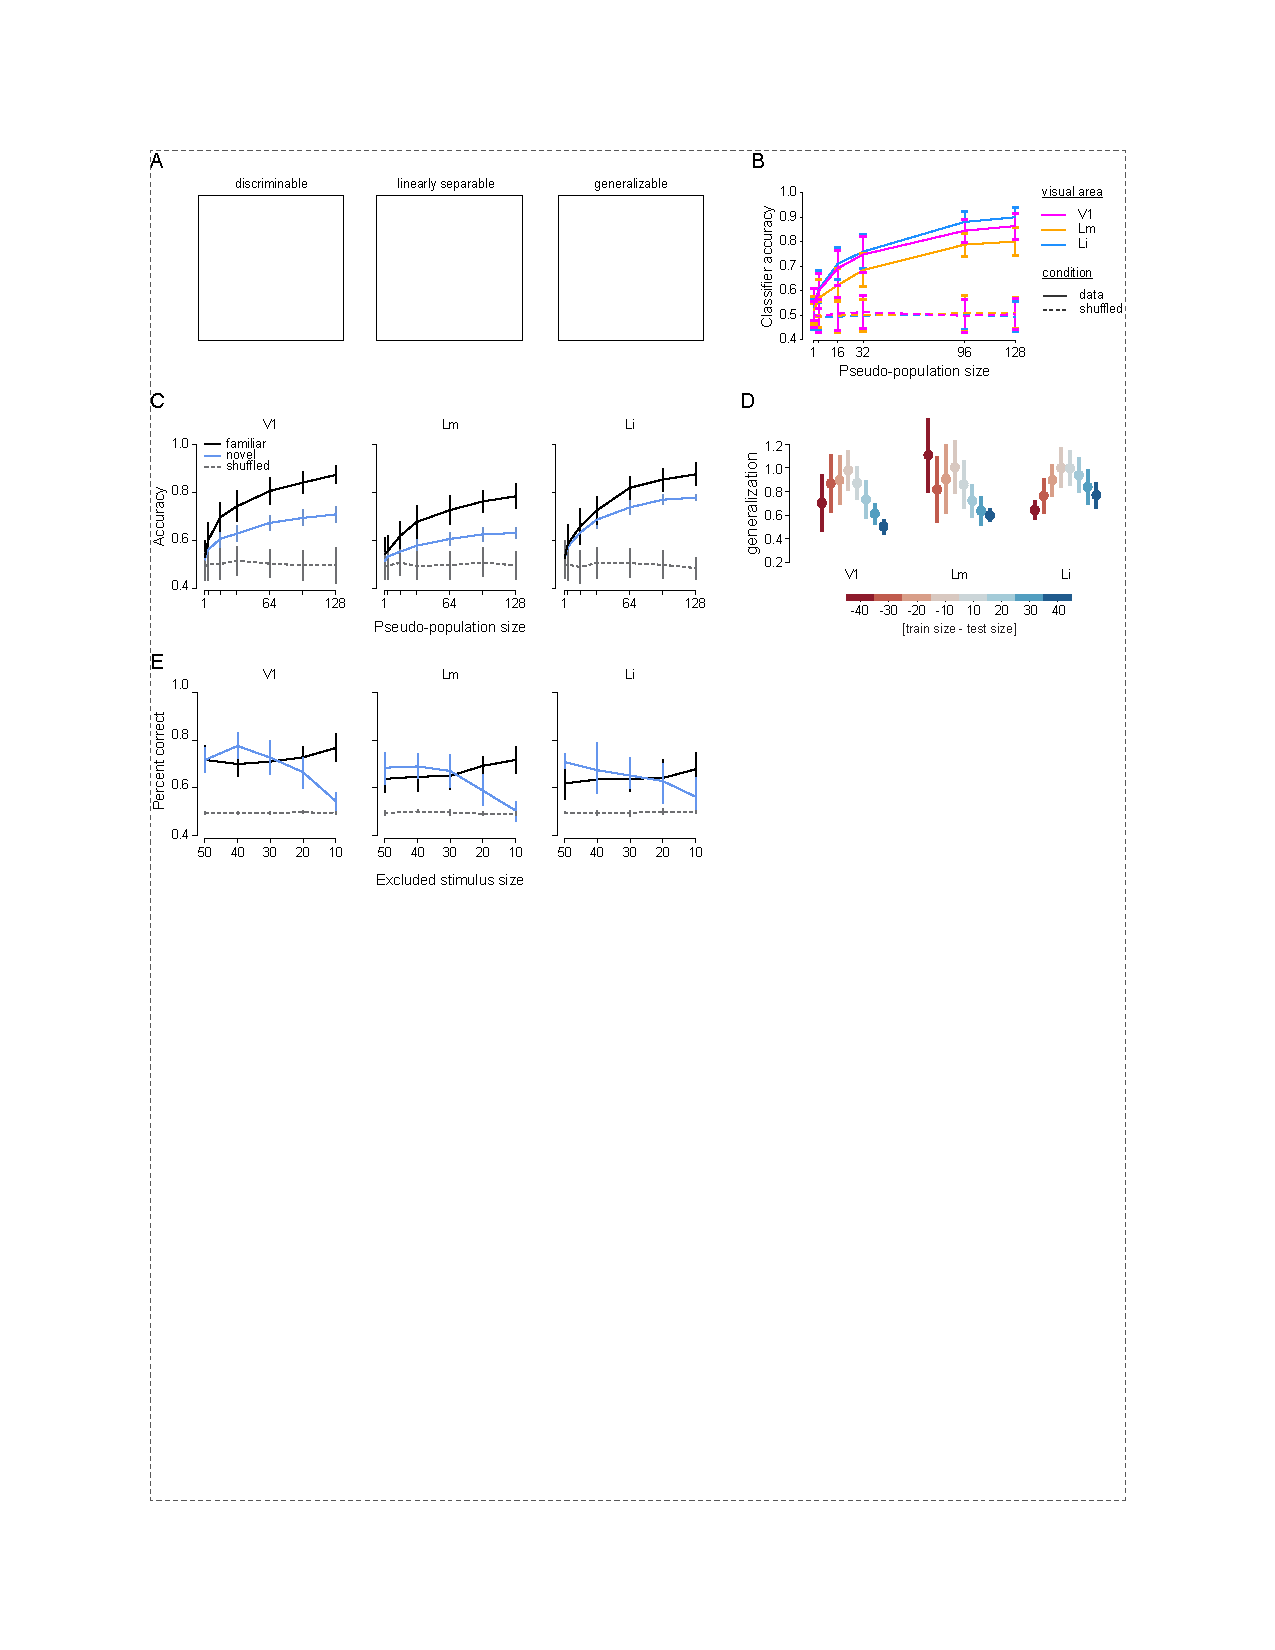
\includegraphics[width=\textwidth]{figures/chapter_4/fig_4-2_neural_generalization/fig_4-2_neural_generalization.pdf}
    %\vspace{.1in}
    \caption[Population representations of objects]{Linear separability and generalization of population representations. 
    \textbf{A.} Schematic of tests for linear separability and generalization (adapted from \cite{Rust2010SelectivityIT}). \textit{Left}: A hypothetical population response for a single presentation of an image as a point in N-dimensional space, where N is the number of neurons in the population (illustrated here in 2D space, for 2 neurons). Different trials of the same image (blue dots) form a “cloud” in this N-dimensional space. The ability of the population to discriminate the different images is proportional to how far apart the response clouds are. Linear classifier approaches identify the optimal hyperplane that separates the responses to one image (blue cloud) from responses to all other images (green cloud). Performance on the discriminability task is measured as the proportion of times that response vectors on test trials correctly fall on the correct side of the hyperplane. \textit{Middle and Right}: Hypothetical representations that perform well or poorly under different tests of linear separability and tolerance. \textif{Middle}: A population that is linearly separable (black cloud separated from gray clouds) and could support generalization under one test (dashed line, “Trained on all conditions”) but fail under another (solid line, “Train on one condition,” and test on the others) with different views of a given object (blue clouds) assigned to the wrong side of the hyperplane. \textit{Right}: A population that is linearly separable and passes tests of generalization when testing on a single reference condition alone.
    \textbf{B.} Linear separability as a function of pseudo-population size (middle panel in \textbf{A}) for V1 (magenta), LM (orange), and LI (blue). Classifiers were trained on responses from all transformations simultaneously, then tested on a subset of trials not included in the training or cross-validation steps. Dotted lines indicate performance when object labels were shuffled. Error bars, bootstrapped estimates of the 95\% CI of the mean accuracy. 
    \textbf{C.} Tolerance as measured by classifier accuracy on generalization tests (right panel in \textbf{A}) as a function of pseudo-population size for V1 (left), LM (middle), and LI (right) populations. Populations were trained at a given stimulus size, then tested on new samples of the same stimulus size (black, “trained” stimulus size) and on samples of stimulus sizes not included in the training set (blue, “novel” stimulus sizes). Dotted lines indicate classifier accuracy when object labels were shuffled. Error bars, bootstrapped estimates of the 95\% CI of the mean accuracy.
    \textbf{D.} Generalization score for novel test conditions, split by the difference between train and test stimulus sizes. Generalization is defined as the ratio of classifier performance on novel conditions to performance on trained conditions (shown for the largest pseudo-population size tested, solid blue and black points at n=128 cells in \textbf{C}, but split by train-test combinations of stimulus size). Colors show stimulus size during training minus stimulus size during testing.
    \textbf{E.} Classifier performance on the generalization task as a function of training conditions for each imaging site (populations of simultaneously imaged cells). Classifiers were trained on the object identification task using a subset of 4 out of 5 stimulus sizes, then tested on different trials of the same stimulus size as training (black) and on trials of the held-out, untrained stimulus size (blue). Error bars show SD across imaging sites for each visual area. Dashed lines show performance when object labels were shuffled. 
    \label{fig:neural_generalization}}
\end{figure}


% Discussion. 


\chapter{Conclusion}
\label{conclusion}

Visual object recognition is a computationally challenging problem that remains unsolved. Most studies are in humans and monkeys, which are experimentally much less tractable. In recent years, rodents have emerged as powerful systems in which to study visual circuits. There are increasingly sophisticated genetic tools, such as cell-type-specific targeting of single cells, and optical imaging techniques, including multi-photon imaging and  holographic stimulation, that are available for studying the neural circuits associated with a given behavior. A growing number of studies in the mouse have demonstrated the power of these tools for functional dissection in mice, from access to and manipulation of genetically-defined cell types to massively large-scaled population recordings during a trained behavior.

Chronic, large-scale, cellular-resolution imaging forms a class of approaches that have proved immensely powerful in dissecting neural circuits. Despite rats’ amazing behavioral capacities, few paradigms exist for applying these methods to visual circuits of head-fixed, behaving rats. While systems that combine freely moving behavior with tethered or wireless recordings are rapidly improving and highly valuable, awake, head-fixed systems are beneficial for careful stimulus delivery, behavioral monitoring, and chronic preparations that allow for longitudinal studies in which the same cells can be tracked across many days.   


\section{Summary of findings} 
\subsection{High-throughput visual behavior in rats}
Rats exhibit complex behaviors in the field and in the lab. Training rats on complicated tasks takes a great deal of time and labor, and there is little standardization across labs. In Chapter 1, we presented a modular, low-cost, and open-source platform for training large cohorts of rats on a range of visual tasks. With our behavior system, we show that large cohorts of rats can be trained, in parallel, on complex object recognition tasks that typically take about a month or less. Using this system, we were also able to measure rats' perceived similarity judgements for stimuli to be used for subsequent neuronal recordings. 

\subsection{Optical imaging systems in awake, head-fixed rats}
Once we were able to demonstrate a slice of the robust visual capacities of rats, we next established a suite of tools for optical imaging in head-fixed rats. In Chapter 2, we described an optimized pipeline that enables a naive, wild-type laboratory rat to be suitable for cellular resolution imaging in visual cortex while it is awake and head-restrained. Moreover, our imaging system allows the same cells in a given FOV to be tracked across multiple days of recording. As yet another benefit provided by rodent models for vision, we also demonstrate the feasibility of imaging multiple visual areas at once, which has not been possible in awake rats yet. Our approach overcomes maybe challenges that have precluded the rat as a standard model for visual circuit study, despite being the most widely-used animal model across biomedical disciplines. 

\subsection{Basic characterizations of rat extrastriate cortex}
As the first demonstration of optical imaging in extrastriate regions of rat cortex, it was important to contribute baseline metrics of neural responses in these areas for the first time with our suite of new tools. Thus, in Chapter 3, we presented a systematic survey of visual response properties across areas V1, LM, and LI. We selected these areas due to their special place in the field of traditional visual neuroscience as one of the first non-primate species in which both behavioral and neurophysiological signatures of invariant object recognition has been found. Consistent with previous studies in both rats and mice, we found increasing receptive field sizes in extrastriate areas. Interestingly, we also observed several forms of anisotropy in the visual field representations of all areas measured. Cortical magnification was greater along elevation than azimuth, meaning that rat visual cortex contains expanded representations of the vertical dimension compared to the horizontal dimension. We also found that receptive fields were elongated along the horizontal axis, raising the possibility that these anistropic receptive fields facilitate a higher resolution representation of the vertical dimension. Finally, we also found asymmetries in retinotopic scatter: although scatter was greater along elevation for all visual areas, it was not proportional to the asymmetric cortical magnification in LM and LI, as it was in V1. Rather, scatter in elevation was lower than expected, suggesting higher fidelity representations in elevation. Together, these findings raise the possibility of an alternative mechanism for enhanced representations in a non-foveating animal. With the development of head-mounted, eye-tracking acquisition systems\cite{Meyer2020, Michaiel2020}, it is possible to explore these observations further in both mice and rats. 

In addition to biased visual field representations, we also found strong axis tuning and selectivity in V1, and consistent with previous studies in mice, there was an over-representation of cells preferring cardinal axes, especially for horizontally-oriented or vertically-moving gratings. Relative to primates, rodents likely experience different visual statistics, and the biases in edge motion and receptive fields could reflect non-uniform changes in the visual field as an animal runs around close to the ground. 

We also found greater direction tuning in LI than we might have expected from a purely higher-order area like monkey IT. Consistent with Vermaercke \textit{et al.} (2014), we found greater direction tuning in LI than in earlier visual areas, whereas there was comparatively lower axis tuning in LI. These results indicate that lateral extrastriate cortex may be more tuned to motion or moving stimuli than a standard ``primate-like'' object recognition pathway. Furthermore, higher shape discriminability, relative to V1, that was observed in both awake rats\cite{Vermaercke2014} and mice\cite{Froudarakis2020}, was measured using moving stimuli. It is possible that visual object recognition in rodents is closely tied to motion statistics --- given that animals navigate in complex, dynamic environments, studies in rats and mice raise the exciting possibility that traditionally separate ideas, such as the ``what'' and ``where'' pathways, might have closer ties than previously appreciated in the primate brain. 

To date, most studies have not found the same, clearly-defined separation between proposed ``layers'' of the rodent visual hierarchy. Although a growing body of evidence supports this idea, it is also likely that there are fundamental differences in how these visual systems are organized. 

\section{Comparison with existing methods}
Typically, rats are used in freely-moving or unrestrained paradigms. Electrophysiology is commonly used in rats, and in awake animals, provides a powerful preparation for studying neural activity in the context of complex and naturalistic behaviors, as the animal need not be restrained. However, chronic access to the same cells across long periods of time, such as over the course of learning, is challenging and difficult to verify. Furthermore, although increasingly higher-density probes may improve the resolution of recording, they can damage neural tissue, and fine-scale, cell-type-specific manipulations are much harder to control (as opposed to, say, holographic stimulation).  

For optical imaging, the larger size of the rat has been advantageous, as head-mounted scopes can be affixed to the skull for chronic, long-term imaging. However, there is usually trade-off between having a small FOV with cellular resolution (head-mountable scope) or a large FOV without cellular resolution (single-photon). Moreover, in order to access lateral cortex on the side of the animal’s head, head-mounted preparations are difficult to maintain in a stable way. Scott \textit{et al.}, (2013) successfully demonstrated the feasibility of voluntary head-fixation for cellular resolution imaging in trained rats. However, this involves time-intensive and laborious training, and data acquisition is less under experimenter control. 

Our study overcomes many of these trade-offs and demonstrates the feasibility of high-resolution, large-FOV imaging with cellular resolution in awake, head-fixed rats. We leverage the head-fixed system to simultaneously track high-resolution video of the animal’s facial movements and behaviors. Although head-fixing the animal comes at the cost of studying neural activity under unnatural conditions, it comes with the benefit of minimizing highly complex behaviors and actions that are irrelevant to the stimuli being investigated. Specifically, this integrated approach allows us to investigate visual object representations in the context of different states of arousal. Typically, animals are not engaged in a fixed position, let alone a fixed behavior state, when interacting with objects in the world. As such, it is important to understand how different behavior states and task conditions modulate the extent to which neural representations can or cannot support complex behavior such as invariant object recognition.


\section{Comparison with previous studies in rodents}
Vermaerke \textit{et al.} (2014) used electrophysiology to record from awake, head-fixed, naive rats, similar to our study. They found that linear decoding accuracy for static images (simple shapes presented at a given position) were best in V1, while LM and LI accuracies were barely above chance. In contrast, matching for the same pseudo-population sizes (N=64 cells), we found discriminability to be comparable across all areas under study (V1, LM, and LI) and well above chance. This could be due to differences in stimuli, as they use simple stimuli composed of oriented edges (such as triangles, squares), while we use slightly more complex, pseudo-3D object stimuli.

Tafazoli \textit{et al.} (2017) also recorded in naive rats with electrophysiology, but used stimuli similar to ours and recorded in anesthetized, head-fixed rats. Overall, they found significant improvements in all metrics tested for area LL, which was not included in our study. However, their findings in areas V1, LM, and LI are consistent with our results. They found that across areas V1, LM and LI, classifier accuracies on tests for linear separability and generalization were comparable, though LI performance was significantly greater than that of V1 and LM. This is consistent with our finding that, of the three areas, LI appears the most robust to generalization tests across size.

Interestingly, they also found that LM accuracies were the worst overall, ~5-8\% lower classifier accuracy than V1 and LI. We find a similar pattern of results, with LM accuracy ~8\% lower than V1 and LI) when matching for pseudo-population size (n=96 cells), as does Vermaerke et al. (2014), with LM performing the worst in discriminating static images. Absolute accuracy levels were higher in our study and Vermaerke et al., compared to accuracy levels reported for a subset of conditions by Tafazoli et al. (pseudo-population, n=96 cells). This could be due to differences in behavioral state (Tafazoli et al. recorded in anesthetized rats) or differences in stimuli (Tafazoli et al average across a much more diverse and complex array of object images). 

\section{Comparison with other species}
Froudarakis \textit{et al.} (2020) is the only study to show that mice may be capable of the type of object recognition tasks used to train rats. Although overall performance in mice falls short of the accuracy levels we find in our trained rats, generalization appears robust. Their study provides a valuable point of comparison as they also record in awake, passively-viewing animals using two-photon imaging.

Unlike most rat studies, Froudarakis et al. used dynamic movie stimuli as opposed to static images while recording in awake, head-fixed mice. Like Vermaerke et al., who also used dynamic movie stimuli, Froudarakis et al. found that discriminability increases from V1 to LM to LI at the level of single neurons -- these single unit results are similar to those of Vermaerke et al. (2014), who found increasing discriminability by another metric of shape selectivity, i.e., sparseness. However, at the population level, the ephys rat studies and imaging mouse study appear to differ, with highest discriminability in LM in the mouse (and area AL, not tested here), and in rats, the worst performance across all metrics for area LM. Froudarakis et al. also find an increase in discriminability as a function of stimulus size. These results are consistent with ours, but only for areas V1 and LM. In area LI, we find that discriminability, as measured by classifier accuracy, is fairly constant across the range of sizes tested. 

Both Froudarakis et al. and Tafazoli et al. tested multiple types of identity-preserving transformations, and consistent with our results, that LI appears more robust to size transformations, both studies find that LI tends to exhibit some improvement beyond V1, depending on the particular transformation. Interestingly, Froudarakis et al. find LM and AL to be the most robust to transformations, whereas this is area LL for Tafazoli et al. Area LL is a region lateral to LI in rats, but not tested in Froudarakis et al, so future studies may help identify additional extrastriate areas that exhibit features thought to be important for visual object recognition.  

\section{Caveats}
Though the present study presented with many technical difficulties, one consistent challenge was consistent identification of area LL. Area LL is notable because previous studies measured electrophysiological responses , There are several possibilities, which we address now. For example, using many injections of viral GCaMP to cover the cranial window proved to be much more time-consuming and less efficient than desired. Small patches in viral expression preclude us from unambiguously identifying similarly small visual areas. This problem can be overcome by recently developed transgenic animals that express GCaMP in all neurons\cite{Scott2018}. It is unlikely that visual responses in area LL were completely unresponsive to any of the stimuli presented, from the cycling bar stimulus and the receptive field tiling protocols, to the drifting gratings and object stimuli. In a subset of animals, we did identify area LL, but only as putative LL, since LL identification here was relative to only one visual area, namely, LM. As quantified by Juavinett \textit{et al.} and others\cite{Juavinett2017}, several of the smaller extrastriate visual areas that are several borders removed from V1, require multiple abutting regions to also be identified for confident estimations. Our surgical and technical developments from Chapter 2 combined with imaging in transgenic rats will likely improve future attempts to reliably identify area LL. 

Compared to previous studies of tolerant object representations in rodent visual cortex, our study presents a limited set of shapes and transformations. As such, it is difficult to identify the extent to which our results are generalizable across different types of transformations. Given that previous studies have shown that there are asymmetries across transformations in separability and generalization, future work can investigate the extent to which there are interactions in the types of tolerant representations a given visual area can support. For example, given that arousal modulates gain and tuning of simple feature detectors like V1 cells, it would be interesting to investigate how arousal modulations of simple features propagates to downstream, high-level representations.

Although we imaged in awake, head-fixed rats, our recordings were in naive, passively viewing animals. Since vision is less of a dominant sensory modality in rodents than it is in monkeys, presenting visual stimuli that have acquired behavioral importance through training may result in significant differences than has been shown in previous object recognition studies in rodents thus far. However, since many of the studies characterizing the hierarchical organization of primate visual cortex have relied on naive monkeys, either passively viewing or engaged in a simple, orthogonal task. As such, recording in naive rodents allows a valuable point of comparison between the species, as they likely experience dramatically different visual statistics during development.


\section{Future Directions}
Currently, mice are one of the most commonly used models in studies that leverage the power of cellular resolution imaging with genetic tools in awake animals. Although rats are an equally popular model system across many fields of neuroscience, such techniques have remained challenging to apply to larger rodent models. One of the most natural extensions of this work is to combine a behavioral task while the rat is head-fixed. Pilot data suggests that rats can and will learn a two-choice discrimination task. While we trained rats using a custom-built, rat-sized version of the International Brain Lab's steering wheel method (Carandini/Harris Labs, UCL), rodents will engage in Go/No-Go and even two-port tasks while head-fixed. Since our rats were calm and rarely showed signs of distress, we do not foresee training and behaving animals as an unsurmountable step. Expanding on this, many of the existing genetic tools used in mice can be used in rats, from cell-specific stimulation to multi-color functional imaging that tracks defined populations of cells over the course of learning or performing a behavior. 

While the present study relies on the advantages of head-fixed preparations and largely static visual stimuli, vision is a dynamic and active process. Thus, an additional important directions is to bring traditional visual studies closer to more naturalistic behaviors. First, many groups have made significant progress imaging with optical imaging in freely moving rats, and a growing number are able to acquire two-photon imaging by mounting small microscopes on the rat's head. Comparing how the animal uses eye- and head-movements during active vision, that is, during freely moving behavior, and how visual representations compare to when animals are exposed to the same visual stimuli in a passive, head-fixed state (i.e., visual playback), may be a promising paradigm to tease apart contributions of active and passive components of vision. In a similar vein, using a continuous-reporting paradigm, such as the steering wheel described above, rats can be trained to use a closed-loop stimulus that it controls with the wheel (or joystick) to generate particular views of a given object. For example, rats can be trained to associate a particular default stimulus view with a reward, after which point, it must use a physical rotation (with the steering wheel) to rotate a new, different view of the object back around to the trained view. Thus, rather than presenting static 2D images of different 3D objects, the head-fixed preparation combined with a self-generated visual stimulus could provide a more direct readout of the animal's perceptual experience, which could be measured simultaneously in the neural population. This would effectively provide an intermediate mode between active and passive vision.


\section{Concluding remarks}
One of the most exciting avenues in systems neuroscience research today is the ability to study neural circuits simultaneously with behavior over the course of learning. Despite rats being the standard model for studies of learning and memory, few studies have been able to track the same cells over time in rats learning these complex tasks. Over a decade ago, Zoccolan et al. (2009) demonstrated that rats are capable of invariant object recognition, a behavior that was long considered to be unique to primates. Ten years later, Froudarakis \textit{et al.} have shown that mice, too, are capable of this complex visual behavior\cite{Froudarakis2020}. Although a great deal has been learned about how a biological system solves this problem, many questions remain that are unfeasible to ask in primates, and rodent models offer a promising alternative by which both general principles and species-specific adaptations can be discovered. 

Over the past decade, a growing number of studies have started to parse out possible functional hierarchies within rodent visual cortex. At present, it remains unclear whether rodent visual areas neatly map onto primate visual areas. In the context of visual object recognition, rodent visual cortex seems less starkly differentiated, although broad principles, such as increasing view tolerance and object discriminability are beginning to emerge. However, investigations into rodents as a model for what is traditionally considered ``high-level'' vision have only just begun. Our study closes a long-standing gap to unlock the rat as a powerful model system for systems neuroscience. 

The technological advancements presented in this work have the potential to unlock a wide range of new experimental directions, enabled by the superior molecular and genetic tools available in rodents. With the groundwork laid out in the previous chapters, we overcome significant barriers to position future studies to ask new, fundamental questions about the nature of visual population representations in cortex, how they change with experience, and how they might be read-out by downstream cortical areas. By approaching these questions with a technique that allows the measurement of responses from a large population of neurons tracked across days, weeks, and months, we are positioned to ask new, fundamentally different questions about the nature of population representations in cortex. This work sits at the vanguard of a growing trend of using rodent models to address questions more traditionally explored in non-human primates.  The cognitive capabilities of rodents have been consistently underestimated, but increasingly, research groups have successfully challenged the notion that high level processes (such as decision making) can only be studied in primates. This project opens the way for future studies to ask new, fundamental questions about cortex that were previously inaccessible using other experimental means. 
\chapter{Methods}
\label{methods}


\section{Visual Stimuli}
\subsection{Objects}
Visual objects were renderings of three-dimensional models built using a ray tracer package POV-Ray (http://www.povray.org/). Each object was defined as a particular configuration and blend of spheres. The particular objects selected for the anchors were modeled to replicate the stimuli used in a previous study\cite{Zoccolan2009}. Figure\ref{REFREF} shows the "default" object views used during phase 1 of training. Objects were rendered with the same light source location and matched to have approximately equal height, width, and area, as defined by the a bounding box surround each object rendering. Object transformations (\textit{e.g.}, in-depth rotation) were generated using custom Python wrappers and the POV-Ray API (REFREFF github morph-pov). 
Morph stimuli were generated by gradually adjusting the relative proportions of each object, by parametrically shifting the spheres defining one object into the spheres defining the other. We used the Euclidean distance in pixel space to quantify the difference between each neighboring pair of images. 

% Materials and methods
All experimental procedures were reviewed and approved by the Harvard Institutional Animal Care and Use Committee. Experiments were performed at Harvard University. 
Animals
Animals used in this study were female Long-Evans rats, 3 months or older, weighing 250-350g (Charles River Laboratories). Rats were housed on a ventilated rack under a 12 hour light:dark cycle with food and water ad libitum, except when water-restricted for behavior training. 

\section{Surgery}
\subsection{Viral injections}
Intracortical injections were made at multiple sites (~5-15 sites per cranial window, spaced ~0.5-1mm apart) using a microinjector (NanoFil, World Precision Instruments REFREF) fit with a 36G beveled needle (NF36BV-2, WPI). A total of 500-750 nl was injected per site at a constant rate of 10-25nl/min at a depth of 750 um below the surface. A high-titre (TITRE) solution of viral vector (AAV9-syn-jGCAMP7f-WPRE, Addgene) was diluted to a final ratio of 2:1 with a 20\% mannitol solution (Sigma-Aldrich, part # REFREF) to promote diffusion. Trace amounts of Fast-Green (Sigma-Aldrich, part #REFREF) were added for visual confirmation of injected solution in the brain.

\subsection{Headplate implantation}
Aseptic surgical technique was followed during all survival surgeries. A headplate and cranial window were implanted in the same surgery as viral injections using methods modified from mouse cranial window procedures \cite{Goldey2014}. Rats were administered dexamethasone (2 mg/kg, REFREF) ~3 hours prior to surgery in order to reduce brain swelling. Rats were anesthetized using isofluorane in 100\% O2 (induction, 3-5\%; maintenance, 1.5-2\%), and placed in a stereotaxic apparatus (Knopf Instruments, Angle Two, Leica REFREF). Eyes were protected from drying out ophthalmic ointment (Puralube), and then covered with surgical drape to protect from direct light. Heart rate, breathing rate, oxygen saturation, and body temperature were measured with a pulse oximeter and commercially available software (PulseOx, Mouseox). Body temperature was maintained at 38%\circ%C with a feedback-controlled heating pad (REFREF). 

The head was shaved, followed by an application of Nair (REFREF) to clear the site of any hair around the incision site. The exposed scalp was cleaned with saline (REFREF), then wiped with three rounds of Povidone-Iodine swabs (Medline, REFREF). A small lidocaine block (<0.5 cc REFREF) was administered along the incision site, which spanned from just behind the ears to the back of the head. After the incision, the skull surface was thoroughly cleaned with hydrogen peroxide (Swan REFREF) and a mixture of citric acid (10\%) and ferric chloride (3\%) (Parkell #S393). A series of small indentations were placed using a small drill (REFREF) all across the cleaned skull to increase surface area and texturize the skull in preparation for adhesives. Prior to head plate attachment, the center of the craniotomy was marked at -7.0 to -8.5 mm AP, 4.5 to 6.5 mm ML, depending on the areas being targeted for each animal. The implant procedure did not require any bone screws or additional supplements to keep the implant stable across months. 

A custom titanium head plate was attached to the skull over the right hemisphere using dental glue (C&B Metabond, Parkell S380). The head plate was placed at 40 degrees relative to Bregma, which matched the orientation of the imaging plane and captured most of the targeted areas of visual cortex. 

\subsection{Cranial window}
After the head plate was securely glued to the skull surface, the wound margin was closed up, while leaving the circular region surrounding the craniotomy site exposed. A 4-5mm craniotomy was performed at the marked site by careful thinning of the bone with a dental drill within the circular area (Aseptico). Care was taken throughout the drilling process to keep the thinned region within the circular boundaries using a pair of surgical calipers (F.S.T. REFREF). Skull thinning was complete once the entire circular region was semi-transparent and blood vessels were clearly visible through the thinned skull. Once the skull was thinned down, the region was kept immersed in sterile saline (REFREF) for the remainder of the surgery. The remaining thinned bone was removed with laminectomy forceps (Fine Science Tools REFREF #). The dura was cut open using a bent 36G needle tip (REFREF) to gently lift up the dura enough to create a small incision point. Flaps of dura were then peeled back with fine forceps or spring scissors to expose the brain surface, and tucked away around the edges of the craniotomy. Intracortical injections were performed after the duratomy (see Viral Injections).

A window composed of stacked glass coverslips (4x4mm, 1x5mm, Warner Instruments, REFREF) bound with optical adhesive (Norland #71) was then placed over the brain surface. The remaining saline was partially absorbed out with sterile eye-spears (REFREF), and the craniotomy was sealed with cyanoacrylate glue (Vetbond, 3M) over a thin layer of sterile saline. Post-operative animals were administered buprenorphine (X mg/kg, REFREF) and carpofen (5 mg/kg, REFREF) daily for 5-7 days following the surgery.

\section{Widefield mapping}
\subsection{Animal preparation}
About 20 minutes prior to the mapping session, animals were anesthetized with isofluorane (5\% induction, 1-1.5\% maintenance) and administered a subcutaneous dose of cholorprothixene (2 mg/kg, Sigma-Aldrich). During the mapping session, animals were kept anesthetized with minimal levels of isofluorane (0.5-1\%). Anesthesia levels were maintained by testing the paw-pinch reflex and monitoring the breathing rate. The left eye facing the monitor was checked between trials to ensure it remained open and stable.

Multi-site viral injections allowed for greater coverage of exposed cortex, but resulted in patchy expression levels in a subset of animals. Animals with ambiguous retinotopic maps were excluded from further study (see AppendixSUP REFREF \ref{suppfig}).

\subsection{Tandem-lens macroscope}
Widefield mapping was done with a tiltable, tandem-lens macroscope\cite{Ratzlaff1991, Kalatsky2003}, composed of a USB 3.0 CCD camera (MantaG033-B, Allied Vision, REFREF) and 2 Nikon lenses (Nikon, 105-mm and 55-mm). Images were acquired at 25 Hz with 3x3 pixel binning (256x492 pixel ½-type sensor REFREF). Epifluorescence illumination was achieved with a 470nm LED (Thorlabs) that was filtered and reflected through a filter cube that housed an excitation filter (REFREF), dichroic mirror (Thorlabs, #REFREF), and emission filter (REFREF). 

Green fluorescence or reflected light was collected and passed through the filter cube then focused on a CCD detector (CAMERA REFREF). Images were acquired at REFREF Hz with REFREF spatial binning using REFREF CAMAPI software and custom python scripts (GIT REFREF). 
% Compare w. Wekselblatt et al. 2016:  Camera lenses allow a relatively high numerical aperture (NA) for light collection, which can also be adjusted easily using the f-stop setting to restrict the NA. This permits a flexible trade-off between sensitivity and depth of field, especially as increased depth of field is useful, given the curvature of the cortical surface. Imaging was generally performed at an f-stop of 5.6. The ratio of the focal lengths of the two lenses determines image magnification. To map 1 cm of cortex across the 2-cm detector (6.5 μm pixels), we chose 50 mm and 105 mm lenses, yielding magnification of 2.1× and 3.1 μm specimen pixels. In practice, we find an effective spatial resolution of ∼25 μm, based on the highest spatial frequencies present in nonbinned images of vascular structure. Binning across spatially oversampled pixels can reduce shot noise by allowing more total photons to be detected with increased illumination or NA. This is a standard practice in intrinsic signal imaging (Kalatsky and Stryker 2003) and is generally applicable at high light levels, where readout noise is negligible compared with photon count noise.

For epifluorescence illumination, we used a 470 nm LED filtered and reflected by a long-pass dichroic mirror, and emitted fluorescence was filtered and captured at an imaging rate of 25Hz. 


\subsection{Visual stimulation}
Visual stimuli were presented using custom Python scripts (git link REFREF) on a 72 inch LCD monitor (LG REFREF). The monitor was centered in front of the left eye, spanning 177 degrees of visual field along azimuth, 67 degrees along elevation.

The mapping protocol consisted of a periodic, moving bar stimulus \cite{Kalatsky2003, Marshel2011} presented to the (left) eye contralateral to the cranial window. The bar subtended 5 degrees of visual angle, and was either presented as a white bar drifting over a black background or an apertured bar containing one of 32 possible natural scene images drifting over a gray background (REFREF). The bar was presented at 0.13 Hz along the azimuth and elevation axes, for a total of 2 (downward, rightward) or 4 (downward, rightward, leftward, upward) conditions. A total of 4-5 repetitions of 10 cycles each were acquired for each direction. 

\subsection{Area segementation}
Raw fluorescence signals were corrected for slow drift by removing the rolling average of each pixel’s time course. The width of the rolling window was set to 2.5 times the length of the stimulation period. For each pixel, the time courses for each trial (10 cycles of the stimulus) were aligned and averaged for each condition (1 of 4 possible directions). We then performed a Fourier spectral analysis on the averaged time series for each pixel to get a magnitude and phase value for each pixel at each frequency. The strength of the response to the stimulus was calculated as the ratio of the Fourier magnitude at the frequency of stimulation to the sum of the magnitudes at all other frequencies \cite{Kalatsky2003, OTHERS}.

Retinotopic maps were created by taking the phase values for all pixels in the image and converting them to Cartesian coordinates that matched the linear position of the bar on the monitor to the phase of the stimulus cycle that corresponded to that position. All maps were smoothed with a Gaussian window (FWHM=$50um$) and masked by applying a threshold to the magnitude ratio.  

\section{Two-photon calcium imaging}

\subsection{Area identification and validation}
We targeted a given two-photon FOV by coregistering blood vessel images to widefield retinotopic maps, which allowed coarse-grained targeting of two-photon sessions. All two-photon imaging sessions began with an anatomical run, in which we acquired a surface level z-stack for fiduciary markers to be used in map registration. For blood vessel images, rats were given subcutaneous injections of SR101 (Sigma-Aldrich REFREF) for visualization in the red channel. If blood vessel images were unavailable, the green channel was used for FOV alignment. 

Two-photon blood vessel images were matched to widefield maps offline. We selected matching points between the two views based on uniquely identifiable blood vessels present in both views, then used these points to identify a transformation matrix to warp one into the other. Assignment of two-photon FOVs were validated based on retinotopic maps measured with the same paradigm used for widefield maps of azimuth and elevation. We generated sign maps from the retinotopic maps with a series of morphological filters\cite{Marshel2011, Garrett2014, Zhuang2017}, which were then used to identify patches representing putative visual areas (Supp Figure? REFREF). Only two-photon FOVs with matches to widefield maps and unambiguous sign reversals were included for subsequent analyses. 

%%%%

Visual stimulation
Retinotopic mapping (area ID)
Receptive field mapping (visual field targeting)
Object stimuli

Data acquisition
Visual stimuli, synced to two-photon acquisition, ScanImage vX.X (REFREF). 
Synced also to face-tracker camera.
Image preprocessing
stuff
Cell mask identification
stuff
Time course extraction and correction
Stuff

Selectivity and tolerance metrics
Neuronal selectivity to morphs was quantified by a morph tuning index (Rainer1998, Zoccolan2007), MT=n-Ri/Rmax/n-1, where Ri is a neuron’s response to the ith morph, Rmaxis the maximum response amongst the morphs, and nis the number morphs. As a measure of response sparseness, MT ranges from 0 (no shape selectivity) to 1 (maximally shape selective). Size tolerance was quantified by normalizing size tuning curves to their maximum values, then averaging those resulting values that were < 1, that is, ST=Rtest/maxRtest, where Rtestis the mean response to a given test size of a neuron’s most preferred object, and . denotes the average across tested sizes where Rtest<maxRtest. 
Population readout
Discriminability
To quantify discriminability (Figure 5b), we trained linear classifiers (support vector machines) to discriminate the two original objects from the neural activity in each area {\fig:Figure5). The linear-readout scheme is important in that it is a simple, biologically plausible processing step that amounts to a thresholded sum taken over weighted synapses {\cite}. This classifier approach does not provide a measure for the total information present in the population, but rather estimates the lower bound on the information explicitly accessible to the population to support the visual task {\cite everyone, Hung2005, Rust2010, etc etc). 

Linear support vector machines (SVMs) were trained to discriminate object A from object B from neural responses. Each presentation of an image produced a population response vector x of size Nx1, such that repeated presentations form a cluster of points in N- dimensional space (Figure 5a, left). The linear readout amounts to finding a linear hyperplane that best separates the response clouds corresponding to each image from those corresponding to all other images. Specifically, the linear readout amounts to: f(x)=wTx + b, where w is a Nx1 vector of the linear weights applied to each of N neurons (defines the orientation of the hyperplane), and b is a scalar that offsets the hyperplane from the origin. To determine the population’s choice about which image was presented, a response vector x (population response to one image) was applied to the classifier, and negative values of f(x) indicate object A and positive values indicate object B. Performance was defined as the proportion of correct answers when asked to classify each image with a held-out test set never included in training. 
The hyperplane and threshold for each classifier was determined by a support vector machine (SVM) using the scikit-learn machine learning library (LinearSVC, version REFREF, cite Pedregosa?). The data were split into train and test sets (20%) after balancing numbers of samples per condition. We used a 5-fold cross-validation procedure on the train set to fit and evaluate each model:  of the trials partitioned for training, models were optimized where the best C={10-3, 10-2, 10-1, 1, 10, 102, 103}that yielded the highest accuracy was chosen. Performance was then assessed with the held-out test set. 
Linear separability and generalization
To test linear separability (Figure 5c), 80% of the trials corresponding to object A and object B for each size were simultaneously combined to train and evaluate the models, while the remaining 20% of trials was used to measure classifier performance. 
To test generalization, two regimes were used. In the first, “Train one, test one” (Figure 5d-e), each classifier was trained to classify object A and B at one of the 5 sizes, then tested on each of the remaining 4 untrained sizes. Each training set (for each size) included 80% of the trials for a given size, while the test sets could contain either the remaining 20% of trials of the same size (test accuracy on “trained” conditions) or 100% of the trials at one of the other sizes (test accuracy on “novel” conditions). 
In the second regime, “Train a subset, test one” (Figure 5f),  each classifier was trained with trials of  4 of the 5 sizes together, then tested with the remaining, untrained size. Each training set was composed of 80% of trials at each of the 4 train sizes. The remaining 20% of trials for each of the 4 train sizes combined to form the held-out test set (test accuracy on “trained” conditions), while 100% of the trials of the remaining 5th size formed the other type of test (test accuracy on “novel” conditions). All combinations of 4 of 5 sizes were used to train different classifiers and test generalization performance on samples of the remaining 5th size.
Population sampling
In analyses in which a given metric, e.g,. classifier accuracy, is presented as a function of the number of neurons in a pseudo-population, we applied a resampling procedure to measure the variability that can be attributed to the particular subpopulation of neurons or particular subset of trials used for training versus testing. On each iteration, we sampled a new subpopulation of neurons that were randomly selected (without replacement) from all cells aggregated across imaging sites and animals, for a given visual area, and trials were randomly assigned for training and testing (without replacement). Error bars were calculated as the SD of classifier performance across 100 iterations. Chance performance was computed by randomly assigning objects or images associated with each response vector and repeating the classification analysis.

Estimation of tuning preferences in cell bodies
Estimation of cells with significant visual responses
stuff
Estimation of retinotopic preferences in cell bodies and neuropil
Preferred retinotopic location 
stuff
Retinotopic responses of neuropil surround cell bodies
The center of each neuropil ring was assigned the value corresponding to the preferred retinotopic location of that neuropil ring, a disk of 10um radius was dilated from the center. Overlapping disks were averaged for preferred retinotopy. The final pixe-wise estimates were the result of spatially smoothing with (ndimage.gaussian_filter, sigma=7 → microns). 

Rate of retinotopic change -- methods from Liang et al., Cell 2018. - “rate of retinotopic change” for smoothed retinotopic map.


Estimation of receptive fields 


Quantification and statistical analysis
(or, does this go with each specific analysis section?)

Estimation

\begin{appendices}
    \chapter{Supplemental Materials}
\label{supplementals}

To do.

% Software list/table
% DeepLabCut \href{https://github.com/DeepLabCut/DeepLabCut}
% MWorks \href{https://mworks.github.io}
% ScanImage 2016 \href{http://scanimage.vidriotechnologies.com}

% Custom software
\href{https://github.com/coxlab/behavior_rig}
\href{https://github.com/julianarhee/morph-pov}

\href{https://github.com/julianrhee/retinotopy-mapper}
\href{https://github.com/julianarhee/acquisition-tools}


% Data numbers 

\begin{table}[h]
 \caption{Data Summary}
  \centering
   \begin{tabular}{lllll}
    \toprule
    Stimulus & Area & Rats & FOVs & Cells   \\
    \midrule
    Moving bar & V1  & 5 & 12 & 1277        \\
               & LM  & 6 & 14 & 530         \\
               & LI  & 4 & 9 & 502          \\
    \midrule
    Receptive Fields & V1  & 11 & 11 & 548  \\
                     & LM  & 8 & 8 & 241   \\
                     & LI  & 10 & 10 & 279    \\
    \midrule
    Gratings & V1  & 7 & 7 & 2211     \\
             & LM  & 8 & 8 & 2084     \\
             & LI  & 7 & 7 & 966     \\
    \midrule
    Objects  & V1  & 9 & 8 & 1028   \\
             & LM  & 10 & 7 & 684   \\
             & LI  & 8 & 7 & 402    \\
    \bottomrule
  \end{tabular}
  \label{tab:data_counts}
\end{table}

% \section{Related to Chapter 3}

% \subsection{Comparison of stimulus size for receptive field measurements}

% \subsection{Demonstration of spherical correction}

% \subsection{Comparison of receptive field and gratings tuning}



% \section{Related to Chapter 4}

% \subsection{Tuning similarity as a function of distance}

% \subsection{Classifier accuracy as a function of receptive overlap}

% \subsection{Classifier generalization, matched for receptive field size}

\end{appendices}

\singlespacing

% the back matter
\clearpage
\bibliography{references}
\addcontentsline{toc}{chapter}{References}
\bibliographystyle{apalike2}

\newpage

% If you do want an image in the colophon:
\begin{figure}
  \vspace{50pt}
  \centering
    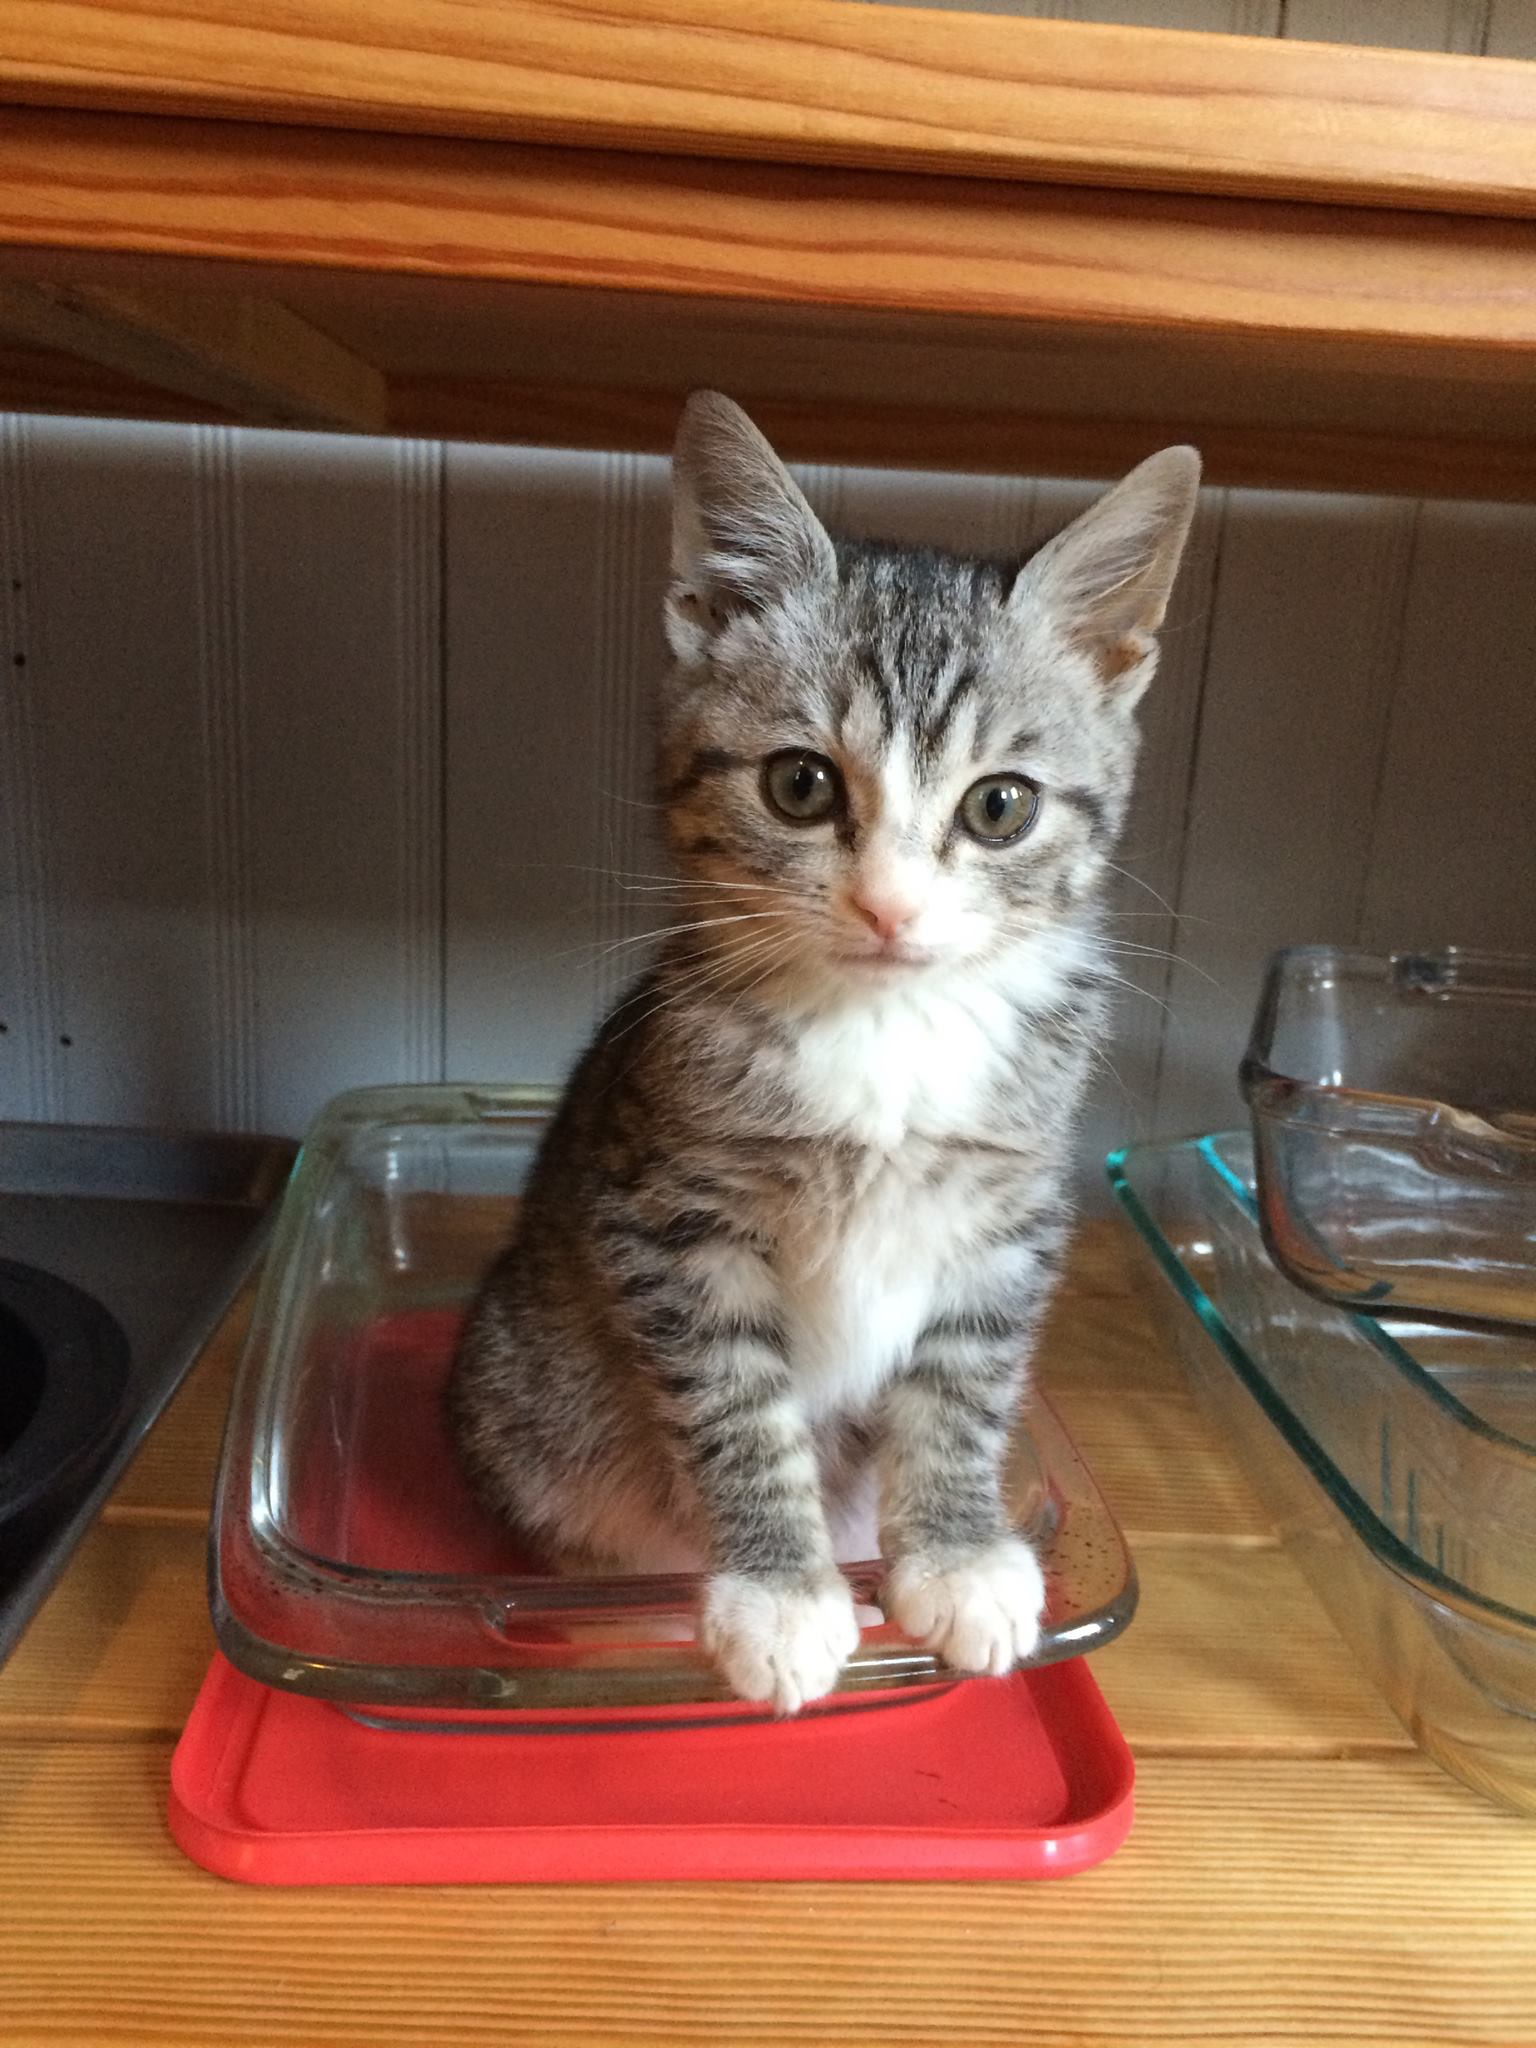
\includegraphics[width=0.51\textwidth]{endmatter/myshka.jpg}
\end{figure}

% If you don't want an image in the colophon:
% \vspace*{200pt}

\begin{center}
\parbox{200pt}{\lettrine[lines=3,slope=-2pt,nindent=-4pt]{\textcolor{SchoolColor}{T}}{his thesis was typeset} using \LaTeX, originally developed by Leslie Lamport and based on Donald Knuth's \TeX. The body text is set in 11 point Egenolff-Berner Garamond, a revival of Claude Garamont's humanist typeface. The above image, taken at Gorham St., is of the most wonderful animal of all, Myshka. A template that can be used to format a PhD thesis with this look and feel has been released under the permissive \textsc{mit} (\textsc{x}11) license, and can be found online at \href{https://github.com/suchow/Dissertate}{github.com/suchow/Dissertate} or from its author, Jordan Suchow, at \href{mailto:suchow@post.harvard.edu}{suchow@post.harvard.edu}.}
\end{center}

\end{document}